\documentclass[12pt,a4paper,twoside]{report}

% ----------------------------
% Pacchetti
% ----------------------------
\usepackage[utf8]{inputenc}
\usepackage[T1]{fontenc}
\usepackage[italian]{babel}
\usepackage{lmodern}
\usepackage{setspace}
\usepackage{geometry}
\usepackage{fancyhdr}
\usepackage{titlesec}
\usepackage{tocloft}
\usepackage{csquotes}
\usepackage{graphicx}
\graphicspath{
  {./}
  {../Iteration_0/}
  {../Iteration_1/}
  {../Iteration_1/Class_Diagram/}
  {../Iteration_1/Sequence_Diagram/V1/}
  {../Iteration_1/Testing/}
  {../Iteration_1/Test_API/}
  {../iteration_2/Sequence_diagram/}
  {../iteration_2/pipelines/}
  {../iteration_2/tests/}
  {../iteration_2/test_API/}
}
\usepackage{hyperref}
\usepackage[all]{hypcap}
\usepackage{float}
\usepackage{caption}
\usepackage{xcolor}
\usepackage{listings}
\usepackage{amsthm}
\usepackage{amsmath}
\usepackage{booktabs}
\usepackage{array}
\usepackage{enumitem}
\usepackage{mdframed}
\usepackage{tabularx}
\usepackage{multirow}
\newtheorem{theorem}{Teorema}[section]

% ----------------------------
% Margini e spaziatura
% ----------------------------
\geometry{a4paper, top=3cm, bottom=3cm, left=3.5cm, right=3cm}
\onehalfspacing
\setlength{\parindent}{1.5em}
\setlength{\parskip}{0pt}

% ----------------------------
% Stile capitoli e paragrafi
% ----------------------------
\titleformat{\chapter}[block]{\normalfont\huge\bfseries}{\thechapter.}{1em}{}
\titlespacing*{\chapter}{0pt}{50pt}{20pt}
\renewcommand{\thechapter}{\arabic{chapter}}
\titleformat{\section}{\normalfont\large\bfseries}{\thesection}{1em}{}
\titlespacing*{\section}{0pt}{18pt}{6pt}
\titleformat{\subsection}{\normalfont\normalsize\bfseries}{\thesubsection}{1em}{}
\titlespacing*{\subsection}{0pt}{12pt}{4pt}
\titleformat{\subsubsection}{\normalfont\normalsize\itshape}{\thesubsubsection}{1em}{}
\titlespacing*{\subsubsection}{0pt}{8pt}{2pt}

% ----------------------------
% Numerazione pagine
% ----------------------------
\pagestyle{fancy}
\fancyhf{}
\fancyhead{}
\fancyfoot[LE]{\thepage}
\fancyfoot[RO]{\thepage}
\fancyfoot[C]{}
\fancypagestyle{plain}{%
  \fancyhf{}
  \fancyhead{}
  \fancyfoot[LE]{\thepage}
  \fancyfoot[RO]{\thepage}
  \fancyfoot[C]{}
}
\renewcommand{\headrulewidth}{0pt}
\renewcommand{\footrulewidth}{0pt}

% ----------------------------
% Stile codice
% ----------------------------
\definecolor{codegreen}{rgb}{0,0.6,0}
\definecolor{codegray}{rgb}{0.5,0.5,0.5}
\definecolor{codepurple}{rgb}{0.58,0,0.82}
\definecolor{backcolour}{rgb}{0.95,0.95,0.92}

\lstdefinestyle{mystyle}{
    backgroundcolor=\color{backcolour},
    commentstyle=\color{codegreen},
    keywordstyle=\color{magenta},
    numberstyle=\tiny\color{codegray},
    stringstyle=\color{codepurple},
    basicstyle=\ttfamily\footnotesize,
    breakatwhitespace=false,
    breaklines=true,
    captionpos=b,
    keepspaces=true,
    numbers=left,
    numbersep=5pt,
    showspaces=false,
    showstringspaces=false,
    showtabs=false,
    tabsize=2
}
\lstset{style=mystyle}

% ----------------------------
% Indice nero (no link colorati)
% ----------------------------
\hypersetup{
  hidelinks,
}

% ----------------------------
% Riquadro per i casi d'uso
% ----------------------------
\definecolor{ucborder}{RGB}{60,90,150}
\definecolor{ucbg}{RGB}{245,247,252}

\newenvironment{ucbox}{%
  \begin{mdframed}[
    backgroundcolor=ucbg,
    linecolor=ucborder,
    linewidth=1pt,
    innerleftmargin=10pt,
    innerrightmargin=10pt,
    innertopmargin=8pt,
    innerbottommargin=8pt,
    roundcorner=4pt
  ]
}{%
  \end{mdframed}
}

% ----------------------------
% Elenchi tool/vantaggi stilizzati
% ----------------------------
\newenvironment{toollist}{%
  \begin{description}[
    style=nextline,
    leftmargin=0pt,
    labelindent=0pt,
    font=\normalfont\bfseries,
    itemsep=6pt
  ]
}{%
  \end{description}
}

% ============================================================
\begin{document}

% ----------------------------
% Frontespizio
% ----------------------------
\begin{titlepage}
\thispagestyle{empty}
    \centering
    
\includegraphics[width=0.26\textwidth, height=3.5cm]{logo_uni.jpg}

    {\Large UNIVERSITÀ DEGLI STUDI DI BERGAMO \\[2cm]}
    {\large \textbf{PAC -- Progettazione Algoritmi e Computabilità} \\[2cm]}

    {\LARGE\bfseries Sfrigo \\[0.5cm]}
    {\large Web App per la Gestione del Frigorifero Condiviso \\[2cm]}

    \begin{minipage}[t]{0.45\textwidth}
        \raggedright
        \textbf{Autori:} \\
        Paganelli Thomas\\
        Matricola n.~1085805\\
        Petrisor Andrei\\
        Matricola n.~1085993\\
        Radu Antonio Valentin\\
        Matricola n.~1085992
    \end{minipage}
    \hfill
    \begin{minipage}[t]{0.45\textwidth}
       \raggedleft
        \textbf{Docente:} \\
        Prof.ssa Scandurra Patrizia \\[0.5cm]
    \end{minipage}

    \vspace{3cm}
    {Anno Accademico 2025/2026}
\end{titlepage}

\newpage
\thispagestyle{fancy}
\mbox{}
\pagenumbering{arabic}

\thispagestyle{fancy}
\tableofcontents

% ============================================================
\chapter{Contesto e Motivazioni}

\section{Contesto Applicativo}

La condivisione di spazi abitativi è una realtà sempre più diffusa, in particolare tra studenti universitari, giovani lavoratori e famiglie allargate. In questi contesti, la gestione delle risorse comuni, e in primo luogo degli alimenti conservati in frigorifero, rappresenta una fonte ricorrente di inefficienze e attriti: alimenti scaduti non vengono rimossi tempestivamente, gli acquisti si duplicano senza necessità, la proprietà dei singoli prodotti è spesso incerta e, in assenza di strumenti adeguati, la comunicazione tra coinquilini è frammentata e informale.

Il problema è aggravato da una tendenza culturale e logistica verso il consumo individuale anche in contesti di convivenza: senza un sistema strutturato, ogni utente tende a gestire i propri alimenti in modo isolato, perdendo l'opportunità di valorizzare le risorse condivise e di ridurre gli sprechi.

\section{Il Problema che Sfrigo Risolve}

\textbf{Sfrigo} nasce per rispondere a una serie di problemi concreti e quotidiani:

\begin{itemize}
  \item \textbf{Spreco alimentare}: in assenza di un sistema di monitoraggio, gli alimenti vengono dimenticati e consumati oltre la data di scadenza. Sfrigo traccia ogni prodotto e lo ordina per urgenza di consumo, riducendo gli sprechi.
  \item \textbf{Mancanza di trasparenza sulla proprietà}: in un frigorifero condiviso non è sempre chiaro quali alimenti appartengano a chi. Sfrigo associa ogni alimento al suo proprietario, garantendo chiarezza e prevenendo conflitti.
  \item \textbf{Difficoltà nella collaborazione culinaria}: cucinare insieme richiede di sapere cosa è disponibile e di chi sono gli ingredienti. Il modulo di generazione ricette di Sfrigo interroga un modello linguistico di grandi dimensioni (LLM) per proporre ricette basate sugli alimenti effettivamente presenti, sia personali che condivisi.
  \item \textbf{Gestione disomogenea dei prodotti condivisi}: alcuni alimenti (sale, olio, condimenti) sono di uso comune, mentre altri sono strettamente personali. Sfrigo consente di marcare esplicitamente la natura di ogni prodotto e di distribuire equamente il contributo di ciascun membro tramite un algoritmo di equità.
  \item \textbf{Assenza di coordinamento nelle abitazioni condivise}: Sfrigo è progettato per abitazioni con più inquilini, residenze universitarie, famiglie e uffici, fornendo un'unica interfaccia che centralizza la gestione del frigorifero e riduce la necessità di comunicazione informale.
\end{itemize}

\section{Obiettivi del Progetto}

L'obiettivo generale del progetto è la realizzazione di una web application che permetta a gruppi di utenti di gestire in modo collaborativo uno o più frigoriferi virtuali condivisi. Nel dettaglio, il sistema si propone di:

\begin{itemize}
  \item Ridurre gli sprechi alimentari attraverso il tracciamento delle scadenze e la prioritizzazione dei consumi.
  \item Facilitare la condivisione degli alimenti tra più utenti con un sistema di proprietà e condivisione trasparente.
  \item Migliorare l'organizzazione del frigorifero tramite categorizzazione, ricerca e ordinamento dinamico degli alimenti.
  \item Supportare la creazione di ricette basate sugli ingredienti disponibili, sfruttando modelli AI generativi.
  \item Garantire equità nella gestione delle risorse condivise tramite un algoritmo di distribuzione dei costi.
\end{itemize}

% ============================================================
\chapter{Componenti del Progetto}

\section{Struttura a Macroblocchi}

Il sistema Sfrigo è articolato in cinque componenti principali, ciascuno con responsabilità ben definite e confini chiari. Questa struttura riflette il pattern architetturale a microservizi adottato, descritto in dettaglio nel capitolo successivo.

\begin{figure}[H]
  \centering
  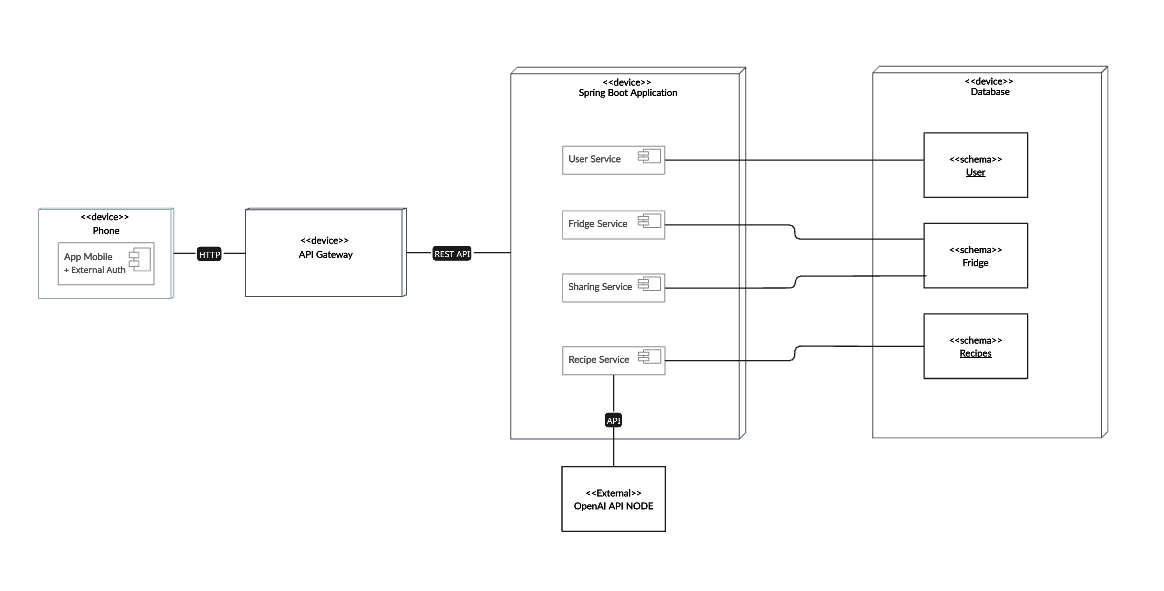
\includegraphics[width=0.9\textwidth, keepaspectratio]{deployment_diagram.PNG}
  \caption{Visione d'insieme dell'architettura del sistema}
  \label{fig:arch_overview}
\end{figure}

\subsection{Frontend -- Next.js Application}

L'interfaccia utente è realizzata come applicazione \textbf{Next.js} (v16), un framework React che supporta sia il rendering lato server (SSR) sia la generazione statica (SSG). Il frontend comunica esclusivamente con l'API Gateway tramite chiamate HTTP autenticate. Le pagine principali includono:
\begin{itemize}
  \item \texttt{/} -- Landing page pubblica
  \item \texttt{/login}, \texttt{/register} -- Autenticazione e registrazione
  \item \texttt{/dashboard} -- Pannello principale con elenco frigoriferi
  \item \texttt{/dashboard/fridge/[id]} -- Vista inventario del singolo frigorifero
  \item \texttt{/invite/[token]} -- Pagina di accettazione inviti
\end{itemize}

\subsection{API Gateway}

Il \textbf{Gateway} è il punto di ingresso unico per tutte le richieste provenienti dal frontend. Le sue responsabilità sono:
\begin{itemize}
  \item Verificare i token JWT emessi da Firebase Authentication, rifiutando le richieste non autenticate.
  \item Iniettare le informazioni sull'utente autenticato (\texttt{X-User-Id}, \texttt{X-User-Email}) negli header delle richieste inoltrate ai microservizi downstream, evitando che ogni servizio debba gestire autonomamente l'autenticazione.
  \item Instradare le richieste al microservizio competente (User Service, Fridge Service, Recipe Service).
\end{itemize}

\subsection{User Service}

Il \textbf{User Service} gestisce il ciclo di vita del profilo utente all'interno del sistema. Sebbene l'autenticazione primaria sia delegata a Firebase, il servizio si occupa di creare e memorizzare il profilo applicativo dell'utente in PostgreSQL al momento della prima registrazione, associando l'UID Firebase a uno username univoco e a un indirizzo email.

\subsection{Fridge Service}

Il \textbf{Fridge Service} (porta 8082) è il microservizio di maggiore complessità e centralità nel sistema. Gestisce:
\begin{itemize}
  \item La creazione, modifica e cancellazione dei frigoriferi virtuali (dati relazionali in PostgreSQL).
  \item La gestione dei membri e dei ruoli (OWNER/MEMBER) all'interno di ogni frigorifero.
  \item Il sistema di inviti tramite token temporanei con scadenza a 24 ore.
  \item L'inventario degli alimenti di ogni frigorifero (dati flessibili in MongoDB).
  \item Il calcolo dell'equità economica tra i membri basato sul valore degli alimenti inseriti.
\end{itemize}

\subsection{Recipe Service}

Il \textbf{Recipe Service} si integra con l'API OpenAI per generare suggerimenti di ricette a partire dagli alimenti disponibili nell'inventario. Riceve una lista di ingredienti selezionati dall'utente, costruisce un prompt strutturato e restituisce le ricette generate dal modello GPT-4o-mini. Il servizio è stateless e non persiste dati propri.

% ============================================================
\chapter{Architettura e Metodologia}

\section{Architettura a Microservizi}

L'architettura adottata è basata sul pattern dei \textbf{microservizi}, in cui il sistema è decomposto in un insieme di servizi indipendenti, ciascuno deployabile e scalabile autonomamente. Ogni microservizio espone le proprie funzionalità tramite \textbf{API REST} e comunica con gli altri esclusivamente attraverso lo strato di rete, senza condivisione diretta di memoria o stato.

Questa scelta architetturale è motivata da una serie di vantaggi concreti che si riflettono sullo sviluppo collaborativo del progetto:

\begin{toollist}
  \item[Sviluppo parallelo e indipendente]
    La suddivisione in servizi con confini netti ha consentito ai membri del team di lavorare su componenti differenti senza interferenze reciproche. Ogni servizio ha il proprio \texttt{package.json}, il proprio ciclo di build e il proprio container Docker, riducendo al minimo le dipendenze trasversali.

  \item[Scalabilità selettiva]
    In un sistema monolitico, è necessario scalare l'intera applicazione anche se il collo di bottiglia riguarda un solo modulo. Con i microservizi, è possibile aumentare le repliche del solo componente sotto carico, ad esempio il Recipe Service durante picchi di richieste all'API OpenAI, senza impattare gli altri servizi.

  \item[Isolamento dei guasti]
    Un malfunzionamento del Recipe Service non pregiudica la disponibilità delle funzionalità di gestione inventario o autenticazione. L'isolamento riduce il rischio di propagazione degli errori all'intero sistema.

  \item[Flessibilità tecnologica]
    Ogni servizio può adottare il database o la libreria più adatta al proprio dominio, come illustrato nella sezione sulla scelta dei database. Nel nostro caso, il Fridge Service utilizza sia PostgreSQL sia MongoDB a seconda della natura dei dati gestiti.

  \item[Deploy e aggiornamento indipendenti]
    La pipeline CI/CD è configurata per rilevare quali servizi sono stati modificati e ricostruire solo i container interessati, riducendo i tempi di deploy e il rischio di regressioni.

  \item[Sicurezza per compartimentazione]
    Il Gateway costituisce l'unico punto di accesso autenticato dall'esterno. I microservizi interni non sono esposti direttamente a Internet e non devono gestire la verifica dei token, riducendo la superficie di attacco.
\end{toollist}

\section{Scelta dei Database: SQL e NoSQL}

Una delle decisioni architetturali più rilevanti del progetto riguarda l'utilizzo \textit{combinato} di un database relazionale e di uno documentale. Questa scelta non è arbitraria, ma deriva dall'analisi della natura dei dati gestiti dal sistema.

\subsection{PostgreSQL -- Dati Relazionali}

\textbf{PostgreSQL} è stato scelto per i dati con struttura fissa e con forti relazioni tra le entità:

\begin{itemize}
  \item \textbf{Utenti} (\texttt{USERS}): ogni utente ha attributi fissi (ID Firebase, username univoco, email, data di creazione). La struttura non varia tra un utente e l'altro.
  \item \textbf{Frigoriferi} (\texttt{FRIDGES}): ogni frigorifero ha un proprietario definito (chiave esterna verso \texttt{USERS}) e attributi stabili.
  \item \textbf{Membri} (\texttt{FRIDGE\_MEMBERS}): la relazione molti-a-molti tra utenti e frigoriferi richiede integrità referenziale, gestione di ruoli e vincoli di unicità su coppie (fridge\_id, user\_id), tutte caratteristiche native dei database relazionali.
  \item \textbf{Inviti} (\texttt{FRIDGE\_INVITATIONS}): i token di invito hanno una scadenza precisa e sono associati a un frigorifero e a un utente creatore; le transazioni ACID garantiscono che un token non possa essere accettato due volte.
\end{itemize}

La scelta di PostgreSQL per questi dati è motivata dalla necessità di \textbf{integrità referenziale}, \textbf{transazionalità ACID}, \textbf{query complesse con JOIN} e \textbf{consistenza forte}, proprietà fondamentali quando si gestiscono permessi e relazioni tra entità.

\subsection{MongoDB -- Dati Eterogenei e Flessibili}

\textbf{MongoDB} è stato scelto per la gestione dell'inventario degli alimenti. La motivazione principale è la \textbf{variabilità dello schema}: un alimento può avere attributi molto diversi a seconda della sua natura. Ad esempio:

\begin{itemize}
  \item Un liquido (latte, olio) avrà \texttt{unit: "litri"} e una \texttt{quantity} decimale.
  \item Un alimento confezionato può avere \texttt{brand}, \texttt{notes}, o informazioni nutrizionali.
  \item I campi \texttt{sharing\_status.is\_common\_use} e \texttt{sharing\_status.is\_available\_for\_loan} formano un oggetto annidato che sarebbe artificialmente normalizzato in un modello relazionale.
  \item Il modulo di generazione ricette beneficia di un documento ricco e denormalizzato: l'LLM riceve l'intero oggetto alimento come contesto, senza necessità di eseguire JOIN per raccogliere attributi sparsi tra più tabelle.
\end{itemize}

MongoDB consente inoltre di aggiungere attributi agli alimenti in future iterazioni (allergie, valori calorici, paese di origine) senza richiedere migrazioni dello schema, rendendolo ideale per un sistema in evoluzione agile.

\section{Toolchain e Motivazioni}

\begin{toollist}
  \item[Next.js (Frontend)]
    Framework React di produzione che supporta SSR, SSG e API Routes. La scelta è motivata dalla necessità di avere rendering ottimizzato per SEO, tempi di caricamento ridotti grazie al pre-rendering, e la possibilità di co-locare logica lato server e lato client nello stesso progetto. Il supporto nativo a Tailwind CSS e alle API Routes semplifica il prototipaggio rapido.

  \item[Express.js (Backend)]
    Framework minimalista e maturo per Node.js, scelto per la sua semplicità di configurazione, l'ecosistema di middleware consolidato e la coerenza con il linguaggio JavaScript già utilizzato nel frontend. La versione 5.x adottata introduce la gestione nativa delle promise nei route handler, riducendo il boilerplate per la gestione degli errori asincroni.

  \item[Firebase Authentication]
    Delegare l'autenticazione a Firebase elimina la necessità di implementare e manutenere un sistema di gestione delle credenziali, della rotazione dei token e del recupero password. Firebase offre provider OAuth integrati (Google, email/password), SDK client per il frontend e SDK Admin per la verifica lato server nel Gateway, con un'affidabilità e una sicurezza superiori a qualsiasi implementazione custom.

  \item[Docker e Docker Compose]
    La containerizzazione garantisce la riproducibilità dell'ambiente tra macchine di sviluppo diverse e semplifica il deploy in produzione. Docker Compose orchestra l'avvio coordinato di tutti i servizi in locale, mentre le immagini multi-stage riducono la dimensione finale dei container escludendo le dipendenze di sviluppo.

  \item[GitHub Actions (CI/CD)]
    La pipeline di integrazione e deploy continuo è implementata tramite GitHub Actions. Il workflow rileva automaticamente quali servizi sono stati modificati (tramite \texttt{paths-filter}), esegue lint e test su ciascuno, costruisce le immagini Docker e le pubblica sul Registry remoto. L'automazione riduce il rischio di errori manuali e garantisce che il codice in produzione sia sempre testato.

  \item[ESLint (Analisi Statica)]
    ESLint è integrato in ogni servizio con la configurazione specifica per Node.js/Next.js, garantendo uniformità dello stile del codice tra i membri del team e rilevando errori comuni come variabili non definite, import mancanti o anti-pattern JavaScript.

  \item[Jest e Supertest (Analisi Dinamica)]
    Jest è il framework di testing de facto per l'ecosistema JavaScript/Node.js, con supporto nativo ai mock, alla generazione di report di coverage e all'integrazione con CI. Supertest consente di testare le API Express senza avviare un server reale, simulando richieste HTTP in memoria con pieno controllo sulle asserzioni delle risposte.

  \item[OpenAI GPT-4o-mini (Generazione Ricette)]
    Il modello GPT-4o-mini è stato scelto per il bilanciamento ottimale tra capacità generative, velocità di risposta e costo per token. La generazione di ricette è un task creativo che non richiede la massima potenza computazionale, rendendo un modello di dimensioni ridotte sufficiente e più economico per un progetto accademico.

  \item[GitHub (Versionamento)]
    Il versionamento è gestito tramite GitHub con un flusso strutturato basato su \textbf{branch per feature} (feature branches), \textbf{Pull Request} con revisione obbligatoria prima del merge su \texttt{main}, e \textbf{Issue} per il tracciamento dei work item di ogni iterazione. I tag di versione identificano i rilasci al termine di ogni sprint. Questo flusso simula le pratiche collaborative dei contesti lavorativi reali.

  \item[Postman (Test API Manuali)]
    Postman è stato utilizzato per il testing esplorativo delle API, in particolare per i componenti che richiedono dipendenze esterne reali (come il Gateway con Firebase) per cui il mock sarebbe eccessivamente complesso. Le collection Postman documentano i casi di test e possono essere eseguite come regression test manuali.
\end{toollist}

\section{Versionamento e Gestione dei Microservizi}

Ogni microservizio è versionato indipendentemente tramite il campo \texttt{version} nel proprio \texttt{package.json} e identificato univocamente nel registro container da un tag corrispondente all'hash del commit Git (\texttt{:sha}), oltre al tag \texttt{:latest}. Questo schema consente il rollback preciso a una versione specifica di un singolo servizio senza dover ricostruire l'intero sistema.

Il repository GitHub è organizzato come \textbf{monorepo}: tutti i servizi risiedono nella stessa repository ma in directory separate, semplificando la gestione delle dipendenze condivise, la revisione incrociata del codice e la tracciabilità delle issue. La pipeline CI/CD sfrutta il rilevamento delle modifiche per evitare rebuild non necessari.

% ============================================================
\chapter{Metodologia di Sviluppo}

\section{Approccio Agile e Framework Scrum}

Per lo sviluppo del progetto è stato adottato un approccio \textbf{agile}, nello specifico il framework \textbf{Scrum}. Questo approccio si differenzia dai modelli tradizionali come il Waterfall, che prevedono uno sviluppo lineare e rigidamente strutturato, favorendo invece un approccio iterativo e incrementale.

Ogni iterazione rappresenta un ciclo di sviluppo completo e autocontenuto, comprensivo di pianificazione, analisi, progettazione, implementazione, test e documentazione. Al termine di ogni sprint viene rilasciato un incremento funzionale del software, consentendo di valutare i progressi e di adattare le priorità in base ai risultati ottenuti.

I pilastri dello Scrum adottati nel progetto sono:
\begin{itemize}
  \item \textbf{Sprint pianificati}: ogni iterazione ha una durata definita con obiettivi chiari stabiliti all'inizio del ciclo.
  \item \textbf{Backlog prioritizzato}: i requisiti sono catalogati e prioritizzati secondo tre livelli (alta, media, bassa), garantendo che le funzionalità core vengano sviluppate prima delle funzionalità accessorie.
  \item \textbf{Team multifunzionale e auto-organizzato}: ogni membro del team partecipa sia alla definizione dei requisiti sia all'implementazione, eliminando la separazione rigida tra ruoli.
  \item \textbf{Review continua}: al termine di ogni iterazione vengono prodotti diagrammi UML aggiornati, test di copertura e documentazione delle API per validare il lavoro svolto.
\end{itemize}

\section{Agile Model Driven Development (AMDD)}

Accanto a Scrum è stato adottato l'\textbf{AMDD} (\textit{Agile Model Driven Development}), un approccio che integra la modellazione UML nel ciclo agile senza imporre la produzione di documentazione esaustiva prima dell'implementazione.

In conformità con i principi AMDD, i modelli vengono creati \textit{just enough} e \textit{just in time}: si produce solo la documentazione necessaria per comprendere meglio un componente o per facilitare la comunicazione nel team, e lo si fa quando serve, non in anticipo su tutta la progettazione. Nel progetto questo si è tradotto in:
\begin{itemize}
  \item Diagrammi dei casi d'uso sviluppati nell'Iterazione 0 per definire i requisiti ad alto livello.
  \item Diagrammi di sequence e component prodotti \textit{durante} o \textit{subito prima} dell'implementazione, come supporto alla progettazione delle API.
  \item Class diagram dei tipi di dato utilizzati come contratto tra frontend e backend.
  \item Diagrammi aggiornati ad ogni iterazione per riflettere l'evoluzione del sistema.
\end{itemize}

\section{DevOps e Integrazione Continua}

Il processo di sviluppo è supportato da una pipeline \textbf{DevOps} automatizzata tramite GitHub Actions. Ad ogni push sul branch \texttt{main}, il workflow esegue automaticamente le seguenti fasi:

\begin{enumerate}
  \item \textbf{Rilevamento delle modifiche}: identifica quali servizi sono stati toccati dal commit per evitare rebuild inutili.
  \item \textbf{Analisi della qualità}: per ogni servizio modificato, esegue la verifica delle dipendenze circolari (Madge), l'analisi statica (ESLint) e i test unitari (Jest).
  \item \textbf{Build e pubblicazione}: costruisce le immagini Docker multi-stage e le pubblica sul Registro remoto con tag \texttt{:latest} e \texttt{:sha}.
\end{enumerate}

Questa automazione garantisce che ogni modifica sul branch principale sia validata prima di essere distribuita, riducendo il rischio di regressioni e semplificando il processo di deploy.

% ============================================================
\chapter{Analisi del Codice}

Per garantire la qualità e l'affidabilità del software, è stata effettuata un'attività di analisi del codice suddivisa in due tipologie: \textbf{analisi statica} e \textbf{analisi dinamica}. L'utilizzo combinato di queste due tecniche consente di individuare errori a diversi livelli: l'analisi statica rileva problemi strutturali senza eseguire il codice, mentre l'analisi dinamica verifica il comportamento effettivo del sistema durante l'esecuzione.

\section{Analisi Statica}

L'analisi statica è effettuata tramite \textbf{ESLint}, configurato con le regole specifiche per Node.js e Next.js. Lo strumento analizza automaticamente il codice JavaScript alla ricerca di:
\begin{itemize}
  \item Errori di sintassi e variabili non definite.
  \item Violazioni delle convenzioni di stile adottate dal team.
  \item Pattern potenzialmente problematici (uso di \texttt{==} invece di \texttt{===}, variabili dichiarate ma non utilizzate, ecc.).
  \item Dipendenze circolari tra moduli, rilevate tramite la libreria \textbf{Madge} integrata nella pipeline CI.
\end{itemize}

ESLint è integrato sia nell'ambiente di sviluppo locale (con feedback in tempo reale nell'editor) sia nella pipeline CI, dove un'analisi fallita blocca il processo di build.

\section{Analisi Dinamica}

L'analisi dinamica è realizzata tramite \textbf{Jest} e \textbf{Supertest}. I test sono applicati principalmente agli endpoint delle API, che rappresentano la logica centrale dell'applicazione.

\textbf{Jest} è stato scelto per:
\begin{itemize}
  \item La facilità di integrazione con Node.js e Next.js.
  \item Il sistema di mock integrato, che consente di sostituire dipendenze esterne (database, servizi terzi) con oggetti controllati durante i test.
  \item La generazione automatica di report di coverage (HTML e LCOV), che mostrano la percentuale di codice coperta dai test.
  \item Il rilevamento automatico dei file di test nella cartella \texttt{\_\_tests\_\_/}.
\end{itemize}

\textbf{Supertest} estende Jest consentendo di simulare richieste HTTP verso le applicazioni Express senza avviare un server reale su una porta di rete, rendendo i test più veloci e indipendenti dall'ambiente.

% ============================================================
\chapter{Iterazione 0}

\section{Analisi dei Requisiti}

L'Iterazione 0 costituisce la fase di avvio del progetto, in cui vengono definiti i requisiti del sistema, analizzati i casi d'uso e progettata l'architettura di alto livello. Non viene prodotto codice funzionante in questa fase; l'obiettivo è stabilire una base solida per le iterazioni successive.

L'analisi dei requisiti ha preso avvio dall'identificazione degli scenari di utilizzo reali del sistema, considerando i diversi profili di utenza (coinquilini, familiari, residenti universitari) e le esigenze specifiche di ciascuno. I requisiti emersi sono stati poi classificati per priorità al fine di orientare la pianificazione degli sprint.

\subsection{Gestione Account e Accesso}

L'accesso all'applicazione è riservato esclusivamente a utenti registrati. Il sistema supporta due modalità di registrazione e autenticazione: tramite form con email e password, oppure tramite provider OAuth esterno (Google). L'autenticazione è gestita da Firebase, che rilascia un token JWT verificato dal Gateway ad ogni richiesta. Ogni utente ottiene uno username univoco che ne consente l'identificazione all'interno dei frigoriferi condivisi.

\subsection{Gestione Frigorifero}

Gli utenti registrati possono creare uno o più frigoriferi virtuali. Il creatore assume automaticamente il ruolo di \textit{Admin del Frigo} (OWNER), con privilegi avanzati quali la modifica delle impostazioni, la gestione dei membri e la cancellazione del frigorifero. Gli altri membri hanno il ruolo di MEMBER.

\subsection{Gestione Membri e Inviti}

L'Admin del Frigo può generare un link di invito temporaneo (valido 24 ore) che consente a qualsiasi utente registrato di unirsi al frigorifero. Il sistema di inviti tramite token garantisce che non siano necessarie autorizzazioni esplicite per ogni singolo invito, semplificando il processo di onboarding.

\subsection{Gestione Inventario}

Tutti i membri possono aggiungere alimenti all'inventario. Il sistema tiene traccia del proprietario di ciascun alimento, della data di scadenza, della categoria, della quantità e di eventuali note. Gli alimenti possono essere marcati come \textit{di uso comune}, rendendoli accessibili a tutti i membri per le ricette condivise.

\subsection{Supporto alla Creazione di Ricette}

Il modulo di generazione ricette integra un LLM (OpenAI GPT-4o-mini) per suggerire ricette basate sugli ingredienti selezionati dall'utente. Le ricette possono essere personali (solo ingredienti dell'utente) o condivise (ingredienti di tutti i membri). Al termine, gli ingredienti utilizzati vengono rimossi dall'inventario. Un algoritmo di equità garantisce una distribuzione bilanciata del contributo degli alimenti tra gli utenti nelle ricette condivise.

\section{Use Case Diagram}

\begin{figure}[H]
  \centering
  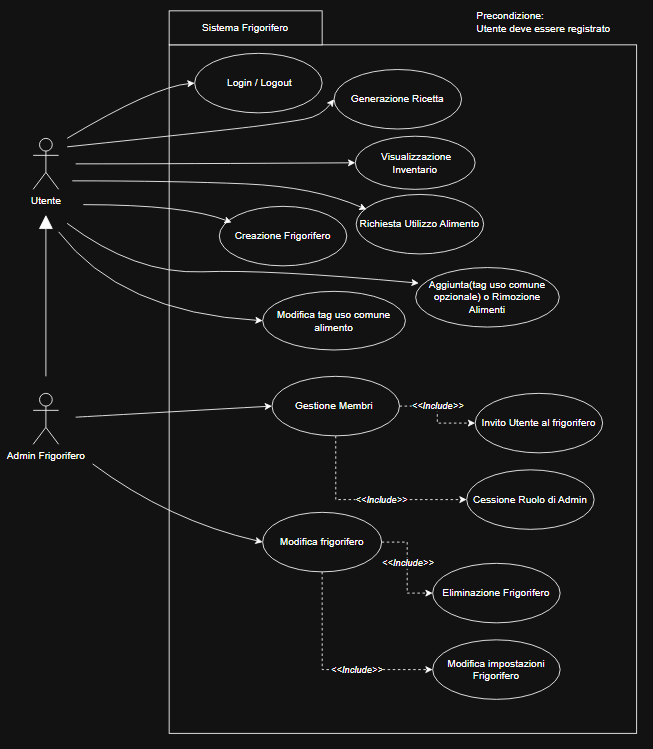
\includegraphics[width=0.75\textwidth]{use_case_diagram.PNG}
  \caption{Diagramma dei Casi d'Uso -- Visione Completa del Sistema}
  \label{fig:use_case}
\end{figure}

\section{Analisi delle Specifiche e Prioritizzazione}

I requisiti identificati sono stati classificati in tre livelli di priorità, seguendo il principio agile di concentrare gli sforzi iniziali sulle funzionalità essenziali per il funzionamento del sistema (\textit{MVP -- Minimum Viable Product}).

\subsection{Alta Priorità}

Le funzionalità di alta priorità costituiscono il nucleo del sistema. Senza di esse l'applicazione non sarebbe utilizzabile e pertanto vengono sviluppate nella prima iterazione.

\begin{center}
\begin{tabular}{@{} l c @{}}
  \toprule
  \textbf{Funzionalità} & \textbf{Codice UC} \\
  \midrule
  Visualizzazione Schermata Iniziale & UC1 \\
  Registrazione Utente               & UC1.1 \\
  Login Utente                       & UC1.2 \\
  Logout Utente                      & UC1.3 \\
  Visualizzazione Dashboard          & UC2 \\
  Creazione Frigorifero              & UC2.1 \\
  Visualizzazione Inventario         & UC3 \\
  Aggiungi Alimento                  & UC3.1 \\
  Rimozione Alimento                 & UC3.2 \\
  Invito al Frigorifero              & UC3.3 \\
  Cancellazione Frigorifero          & UC3.4 \\
  \bottomrule
\end{tabular}
\end{center}

\subsection{Media Priorità}

Le funzionalità di media priorità arricchiscono l'esperienza utente e introducono le caratteristiche collaborative avanzate del sistema. Vengono sviluppate nella seconda iterazione.

\begin{center}
\begin{tabular}{@{} l c @{}}
  \toprule
  \textbf{Funzionalità} & \textbf{Codice UC} \\
  \midrule
  Alimenti di Uso Comune              & UC5 \\
  Tracciamento Proprietario Alimento  & UC6 \\
  Richiesta Ricetta Personale         & UC7 \\
  Ricetta Condivisa                   & UC8 \\
  Algoritmo di Sorting                & UC9 \\
  Algoritmo di Equità                 & UC10 \\
  Gestione Uscita Volontaria da Frigo & UC11 \\
  Rimozione Utente da Frigo           & UC12 \\
  \bottomrule
\end{tabular}
\end{center}

\subsection{Bassa Priorità}

Funzionalità accessorie o migliorative, non sviluppate nelle iterazioni correnti ma incluse nel backlog per sviluppi futuri.

\begin{center}
\begin{tabular}{@{} l @{}}
  \toprule
  \textbf{Funzionalità} \\
  \midrule
  Prestito Alimenti \\
  Sistema di Notifiche Push \\
  Cronologia Consumi \\
  Preferenze Alimentari e Allergie \\
  Supporto Multilingua \\
  Statistiche Avanzate sui Consumi \\
  \bottomrule
\end{tabular}
\end{center}

\section{Analisi dell'Architettura -- Deployment Diagram}

In questa fase viene progettata l'architettura di deployment del sistema, identificando i nodi fisici/logici e le loro interazioni. Il diagramma è volutamente ad alto livello poiché alcune scelte tecnologiche (es. tipo di database) sono ancora da definire.

\begin{figure}[H]
  \centering
  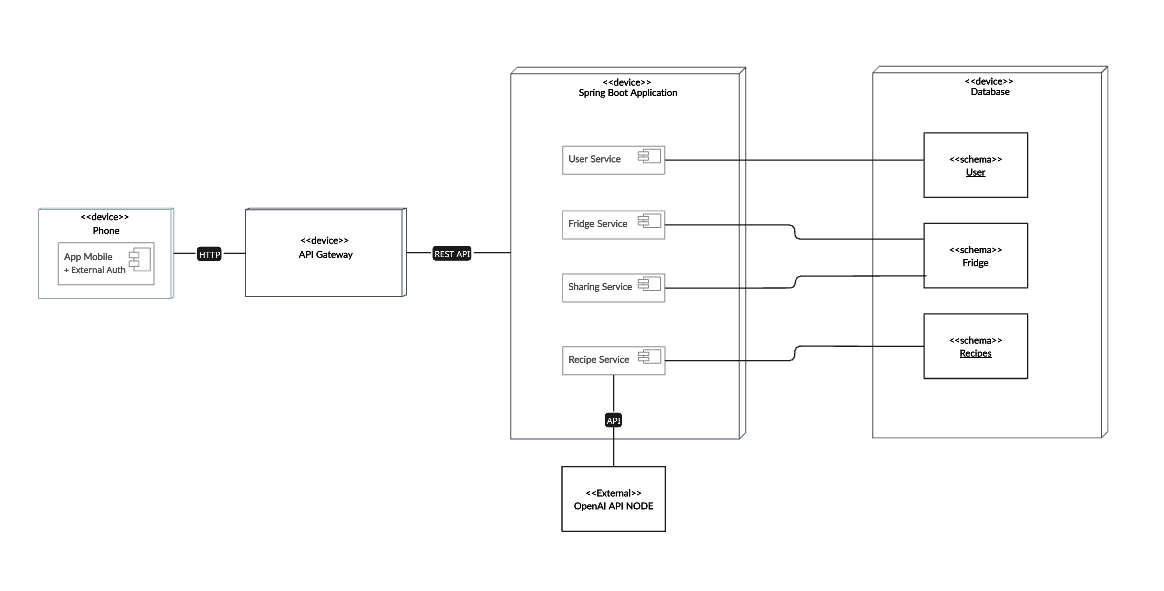
\includegraphics[width=\textwidth, height=\textheight, keepaspectratio]{deployment_diagram.PNG}
  \caption{Diagramma di Deployment -- Iterazione 0}
  \label{fig:deployment}
\end{figure}

\begin{quote}
\textit{Note:} Nel primo nodo (da sinistra) è indicato \textbf{App Mobile + External Auth}, poiché la registrazione e l'autenticazione vengono gestite tramite servizio esterno (Firebase). Il \textbf{Recipe Service} è collegato a un blocco esterno per la generazione delle ricette tramite LLM. Il database è indicato genericamente come \textit{DataBase}, in attesa della scelta definitiva sulla tecnologia da adottare (definita come PostgreSQL + MongoDB nell'Iterazione 1).
\end{quote}

% ============================================================
\chapter{Iterazione 1}

\section{Introduzione}

La prima iterazione ha come obiettivo la realizzazione del nucleo funzionale dell'applicazione, ovvero l'insieme minimo di funzionalità senza le quali il sistema non sarebbe utilizzabile. I work item selezionati per questo sprint corrispondono a tutti i casi d'uso di alta priorità identificati nell'Iterazione 0, e seguono una dipendenza logica precisa: prima di poter gestire frigoriferi e alimenti, è necessario disporre di un sistema di autenticazione funzionante; prima di interagire con l'inventario, è necessario che un frigorifero esista e che l'utente ne faccia parte.

Il percorso di sviluppo parte quindi dall'autenticazione (\textbf{UC1}), che abilita l'accesso all'applicazione tramite registrazione, login con email/password o provider Google, e logout. Una volta autenticato, l'utente accede alla \textbf{Dashboard} (UC2), punto centrale di navigazione da cui è possibile creare nuovi frigoriferi (UC2.1) e accedere a quelli esistenti. Dall'inventario di un frigorifero (\textbf{UC3}) l'utente può aggiungere e rimuovere alimenti (UC3.1, UC3.2), invitare altri utenti tramite link temporaneo (UC3.3) ed eliminare l'intero frigorifero se ne è il proprietario (UC3.4).

\begin{center}
\begin{tabular}{@{} l l @{}}
  \toprule
  \textbf{Caso d'uso} & \textbf{Funzionalità} \\
  \midrule
  UC1    & Visualizzazione Schermata Iniziale \\
  UC1.1  & Registrazione Utente \\
  UC1.2  & Login Utente \\
  UC1.3  & Logout Utente \\
  UC2    & Visualizzazione Dashboard \\
  UC2.1  & Creazione Frigorifero \\
  UC3    & Visualizzazione Inventario \\
  UC3.1  & Aggiunta Alimento \\
  UC3.2  & Rimozione Alimento \\
  UC3.3  & Invito al Frigorifero \\
  UC3.4  & Cancellazione Frigorifero \\
  \bottomrule
\end{tabular}
\end{center}

Parallelamente all'implementazione, vengono prodotti i diagrammi UML di componenti, sequence e class, viene eseguita l'analisi statica tramite ESLint e quella dinamica tramite Jest e Supertest, e le API vengono documentate e verificate tramite Postman.

\section{Descrizione dei Casi d'Uso}

\subsection{UC1 -- Visualizzazione Schermata Iniziale}

\begin{ucbox}
\textbf{Descrizione:} All'apertura della web app l'utente visualizza la pagina di benvenuto, che presenta le funzionalità principali dell'applicazione e fornisce i link per accedere alla registrazione e al login. Se l'utente ha già effettuato il login, viene reindirizzato direttamente alla Dashboard.

\begin{description}[leftmargin=4cm, style=sameline]
  \item[Attori Coinvolti:] Tutti gli utenti (autenticati e non)
  \item[Precondizione:] Nessuna
  \item[Postcondizione:] Corretta visualizzazione della Schermata Iniziale
\end{description}
\end{ucbox}

\textbf{Svolgimento standard:}
\begin{enumerate}
  \item L'utente si collega all'URL della web app.
  \item Il sistema verifica se è presente un token di sessione valido.
  \item Se non autenticato, viene mostrata la landing page con le opzioni di login e registrazione.
\end{enumerate}

\newpage
\subsection{UC1.1 -- Registrazione Utente}

\begin{ucbox}
\textbf{Descrizione:} L'utente non registrato compila il form di registrazione inserendo email, password, nome e cognome, oppure si registra tramite il provider OAuth di Google. Il sistema crea il profilo Firebase e, in caso di successo, persiste il profilo applicativo nel database tramite il User Service.

\begin{description}[leftmargin=4cm, style=sameline]
  \item[Attori Coinvolti:] Utente non registrato
  \item[Precondizione:] Utente non già registrato con la stessa email
  \item[Postcondizione:] Profilo utente creato in Firebase e in PostgreSQL; utente reindirizzato alla Dashboard
  \item[Trigger:] L'utente clicca il link \textit{``Register''} dalla schermata iniziale o dalla pagina di login
\end{description}
\end{ucbox}

\textbf{Svolgimento standard:}
\begin{enumerate}
  \item L'utente clicca su \textit{``Register''} e viene reindirizzato alla pagina di registrazione.
  \item L'utente inserisce i propri dati nel form oppure utilizza il pulsante \textit{``Accedi con Google''}.
  \item Il sistema invia la richiesta a Firebase Authentication.
  \item Firebase crea il profilo di autenticazione e restituisce un token JWT.
  \item Il sistema invoca il User Service per creare il profilo applicativo in PostgreSQL.
  \item L'utente viene reindirizzato alla Dashboard.
\end{enumerate}

\textbf{Svolgimento alternativo:}
\begin{enumerate}
  \item L'utente inserisce un'email già presente nel sistema.
  \item Firebase restituisce un errore di email già in uso.
  \item Il sistema notifica l'utente e lo invita a effettuare il login o a utilizzare un'email diversa.
\end{enumerate}

\newpage
\subsection{UC1.2 -- Login Utente}

\begin{ucbox}
\textbf{Descrizione:} L'utente registrato inserisce le proprie credenziali (email e password) nel form di login oppure utilizza il provider Google. In caso di credenziali corrette, Firebase restituisce un token JWT che viene conservato localmente e allegato a ogni richiesta successiva verso il Gateway.

\begin{description}[leftmargin=4cm, style=sameline]
  \item[Attori Coinvolti:] Utente registrato non autenticato
  \item[Precondizione:] Utente non loggato
  \item[Postcondizione:] Utente loggato; token JWT memorizzato lato client; reindirizzamento alla Dashboard
  \item[Trigger:] L'utente clicca il link \textit{``Accedi''} dalla schermata iniziale
\end{description}
\end{ucbox}

\textbf{Svolgimento standard:}
\begin{enumerate}
  \item L'utente clicca su \textit{``Accedi''} e viene reindirizzato alla pagina di login.
  \item L'utente inserisce email e password oppure utilizza \textit{``Continua con Google''}.
  \item Il sistema invia le credenziali a Firebase Authentication.
  \item Firebase verifica le credenziali e restituisce un token JWT.
  \item Il client memorizza il token e reindirizza l'utente alla Dashboard.
  \item In caso di credenziali errate, il sistema mostra un messaggio di errore e invita a riprovare.
\end{enumerate}

\newpage
\subsection{UC1.3 -- Logout Utente}

\begin{ucbox}
\textbf{Descrizione:} L'utente può disconnettersi volontariamente o il sistema effettua il logout automatico allo scadere della sessione Firebase.

\begin{description}[leftmargin=4cm, style=sameline]
  \item[Attori Coinvolti:] Utente autenticato
  \item[Precondizione:] Utente loggato
  \item[Postcondizione:] Token invalidato; utente reindirizzato alla schermata iniziale
  \item[Trigger:] Clic sul pulsante di logout oppure scadenza del token di sessione
\end{description}
\end{ucbox}

\textbf{Svolgimento standard:}
\begin{enumerate}
  \item L'utente clicca sull'icona del profilo e seleziona \textit{``Logout''}.
  \item Il sistema invoca il metodo di sign-out di Firebase, che invalida il token lato client.
  \item L'utente viene reindirizzato alla pagina iniziale.
\end{enumerate}

\textbf{Svolgimento alternativo (logout automatico):}
\begin{enumerate}
  \item Il token di sessione Firebase scade.
  \item Il sistema rileva l'assenza di un token valido alla successiva richiesta autenticata.
  \item L'utente viene reindirizzato alla pagina di login.
\end{enumerate}

\newpage
\subsection{UC2 -- Visualizzazione Dashboard}

\begin{ucbox}
\textbf{Descrizione:} La Dashboard è la pagina principale per gli utenti autenticati. Mostra tutti i frigoriferi a cui l'utente appartiene (come OWNER o MEMBER) e consente di creare nuovi frigoriferi o accedere all'inventario di quelli esistenti.

\begin{description}[leftmargin=4cm, style=sameline]
  \item[Attori Coinvolti:] Utente autenticato
  \item[Precondizione:] Utente loggato
  \item[Postcondizione:] Corretta visualizzazione della Dashboard con l'elenco dei frigoriferi
  \item[Trigger:] Login avvenuto con successo oppure navigazione diretta alla route \texttt{/dashboard}
\end{description}
\end{ucbox}

\textbf{Svolgimento standard:}
\begin{enumerate}
  \item L'utente accede alla Dashboard (automaticamente dopo il login o navigando a \texttt{/dashboard}).
  \item Il frontend invia una richiesta GET autenticata al Gateway per ottenere l'elenco dei frigoriferi dell'utente.
  \item Il sistema mostra i frigoriferi con nome, ruolo dell'utente e data di creazione.
\end{enumerate}

\newpage
\subsection{UC2.1 -- Creazione Frigorifero}

\begin{ucbox}
\textbf{Descrizione:} L'utente autenticato può creare un nuovo frigorifero virtuale assegnandogli un nome. Il sistema crea il record in PostgreSQL, assegna all'utente il ruolo di OWNER e aggiunge automaticamente l'utente come membro.

\begin{description}[leftmargin=4cm, style=sameline]
  \item[Attori Coinvolti:] Utente autenticato
  \item[Precondizione:] Utente loggato
  \item[Postcondizione:] Nuovo frigorifero creato; utente aggiunto come OWNER; frigorifero visibile nella Dashboard
  \item[Trigger:] Clic sul pulsante \textit{``Nuovo Frigo''}
\end{description}
\end{ucbox}

\textbf{Svolgimento standard:}
\begin{enumerate}
  \item L'utente clicca su \textit{``Nuovo Frigo''} nella Dashboard.
  \item Il sistema mostra un form per l'inserimento del nome del frigorifero.
  \item L'utente inserisce un nome e conferma.
  \item Il sistema invia una POST al Gateway, che la instrada al Fridge Service.
  \item Il Fridge Service crea il record frigorifero in PostgreSQL e aggiunge l'utente come OWNER.
  \item Il nuovo frigorifero appare nella Dashboard.
\end{enumerate}

\newpage
\subsection{UC3 -- Visualizzazione Inventario}

\begin{ucbox}
\textbf{Descrizione:} Accedendo a un frigorifero, l'utente visualizza l'inventario degli alimenti presenti, l'elenco dei membri, e ha accesso alle azioni disponibili (aggiunta/rimozione alimenti, invito, gestione del frigo).

\begin{description}[leftmargin=4cm, style=sameline]
  \item[Attori Coinvolti:] Utente membro del frigorifero
  \item[Precondizione:] Utente loggato e membro del frigorifero
  \item[Postcondizione:] Visualizzazione completa dell'inventario e dei dati del frigorifero
  \item[Trigger:] Clic su un frigorifero nella Dashboard
\end{description}
\end{ucbox}

\subsection{UC3.1 -- Aggiungi Alimento}

\begin{ucbox}
\textbf{Descrizione:} L'utente inserisce un nuovo alimento nell'inventario del frigorifero. I dati dell'alimento (nome, categoria, quantità, unità, scadenza) vengono salvati in MongoDB; l'ID dell'utente viene automaticamente associato all'alimento come proprietario.

\begin{description}[leftmargin=4cm, style=sameline]
  \item[Attori Coinvolti:] Utente membro del frigorifero
  \item[Precondizione:] Utente loggato e membro del frigorifero
  \item[Postcondizione:] Alimento creato in MongoDB e visibile nell'inventario
  \item[Trigger:] Clic sul pulsante \textit{``Aggiungi Alimento''}
\end{description}
\end{ucbox}

\textbf{Svolgimento standard:}
\begin{enumerate}
  \item L'utente clicca su \textit{``Aggiungi Alimento''}.
  \item Il sistema mostra un form con i campi: nome, categoria, quantità, unità, data di scadenza, note, stato di condivisione.
  \item L'utente compila il form e clicca \textit{``Aggiungi''}.
  \item Il frontend invia una POST autenticata al Gateway.
  \item Il Fridge Service persiste il documento in MongoDB, associando l'ID utente come owner.
  \item L'alimento appare nell'inventario.
\end{enumerate}

\newpage
\subsection{UC3.2 -- Rimozione Alimento}

\begin{ucbox}
\textbf{Descrizione:} L'utente può rimuovere un alimento dall'inventario. Di norma ogni utente può eliminare solo i propri alimenti; l'Admin del Frigo può rimuovere qualsiasi alimento.

\begin{description}[leftmargin=4cm, style=sameline]
  \item[Attori Coinvolti:] Utente proprietario dell'alimento o Admin del Frigo
  \item[Precondizione:] Utente loggato; alimento presente nell'inventario
  \item[Postcondizione:] Alimento rimosso dal documento MongoDB
  \item[Trigger:] Clic sul pulsante \textit{``Elimina Alimento''}
\end{description}
\end{ucbox}

\textbf{Svolgimento standard:}
\begin{enumerate}
  \item L'utente clicca su un alimento nell'inventario.
  \item Il sistema mostra i dettagli dell'alimento con il pulsante \textit{``Elimina Alimento''}.
  \item L'utente clicca su \textit{``Elimina Alimento''} e conferma.
  \item Il Fridge Service rimuove il documento da MongoDB.
\end{enumerate}

\newpage
\subsection{UC3.3 -- Invito al Frigo}

\begin{ucbox}
\textbf{Descrizione:} L'Admin del Frigo può generare un link di invito con scadenza a 24 ore. Chiunque abbia il link e sia registrato al sistema può unirsi al frigorifero accedendo all'URL di invito.

\begin{description}[leftmargin=4cm, style=sameline]
  \item[Attori Coinvolti:] Admin del Frigo (generazione); qualsiasi utente registrato (accettazione)
  \item[Precondizione:] Utente loggato con ruolo OWNER nel frigorifero
  \item[Postcondizione:] Token di invito generato in PostgreSQL; l'utente che accetta il link viene aggiunto come MEMBER
  \item[Trigger:] Clic sul pulsante \textit{``Invita''}
\end{description}
\end{ucbox}

\textbf{Svolgimento standard:}
\begin{enumerate}
  \item L'utente Admin clicca su \textit{``Invita''} nell'inventario del frigorifero.
  \item Il sistema genera un token UUID, lo persiste in \texttt{FRIDGE\_INVITATIONS} con scadenza a 24 ore, e costruisce l'URL di invito.
  \item L'utente condivide il link con i potenziali membri.
  \item Il destinatario accede al link \texttt{/invite/[token]}, effettua il login se necessario, e clicca \textit{``Accetta Invito''}.
  \item Il Fridge Service verifica la validità del token, aggiunge l'utente come MEMBER e invalida il token.
\end{enumerate}

\newpage
\subsection{UC3.4 -- Rimozione Frigorifero}

\begin{ucbox}
\textbf{Descrizione:} L'Admin del Frigo può eliminare definitivamente il frigorifero, rimuovendo tutti i dati associati (membri, inviti, alimenti) sia da PostgreSQL sia da MongoDB.

\begin{description}[leftmargin=4cm, style=sameline]
  \item[Attori Coinvolti:] Admin del Frigo (ruolo OWNER)
  \item[Precondizione:] Utente loggato con ruolo OWNER
  \item[Postcondizione:] Frigorifero e tutti i dati correlati eliminati; frigorifero rimosso dalla Dashboard
  \item[Trigger:] Clic sul pulsante \textit{``Elimina Frigorifero''}
\end{description}
\end{ucbox}

\textbf{Svolgimento standard:}
\begin{enumerate}
  \item L'utente Admin accede all'inventario del frigorifero.
  \item L'utente clicca su \textit{``Elimina Frigorifero''} e conferma l'operazione.
  \item Il Fridge Service rimuove il record da \texttt{FRIDGES} (con cascade su \texttt{FRIDGE\_MEMBERS} e \texttt{FRIDGE\_INVITATIONS}) e tutti i documenti degli alimenti da MongoDB.
  \item Il frigorifero scompare dalla Dashboard di tutti i membri.
\end{enumerate}

\newpage
\section{Component Diagram}

Il \textbf{Component Diagram} UML rappresenta la struttura architettonica del sistema in termini di componenti software e delle loro interdipendenze. Ogni blocco rappresenta un modulo deployabile (frontend, gateway, microservizi, database), mentre le frecce indicano le dipendenze e i canali di comunicazione tra di essi. Nel contesto di questa iterazione, il diagramma riflette l'architettura completa del sistema, incluse le tecnologie definitivamente scelte per i database.

\begin{figure}[H]
  \centering
  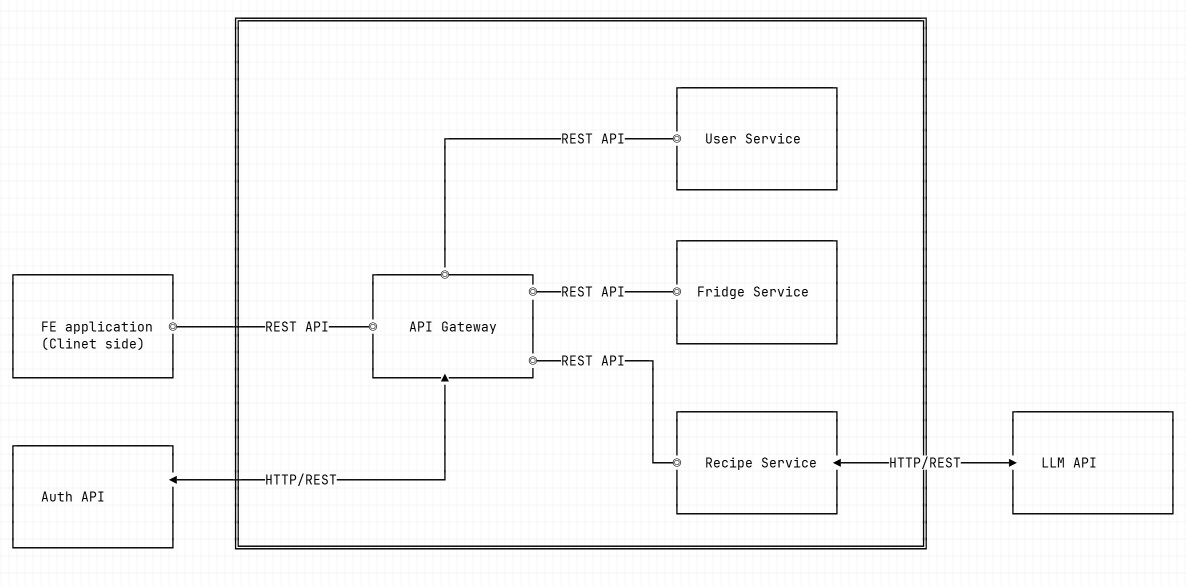
\includegraphics[width=\textwidth, height=\textheight, keepaspectratio]{Component_Diagaram_V1.jpg}
  \caption{Component Diagram -- Iterazione 1}
  \label{fig:component}
\end{figure}

\section{UML Sequence Diagram}

I \textbf{Sequence Diagram} UML illustrano le interazioni temporali tra i componenti del sistema durante l'esecuzione di una specifica funzionalità. Ogni elemento è rappresentato da una \textit{lifeline} verticale, mentre le frecce orizzontali indicano i messaggi scambiati. Il tempo scorre dall'alto verso il basso. Questi diagrammi sono particolarmente utili per visualizzare il flusso di una richiesta dall'utente fino al database, passando per frontend, gateway e microservizi.

\textit{Tool utilizzato per la realizzazione: MonoSketch.}

\newpage

\subsection{Autenticazione}

Il diagramma descrive il flusso di autenticazione dell'utente tramite Firebase. Il client invia le credenziali direttamente all'SDK Firebase, che restituisce un token JWT firmato. Nelle richieste successive, il token viene allegato nell'header \texttt{Authorization} e verificato dal Gateway tramite Firebase Admin SDK prima di essere inoltrato ai microservizi. I microservizi non eseguono alcuna verifica autonoma: ricevono le informazioni sull'utente già estratte dal Gateway negli header \texttt{X-User-Id} e \texttt{X-User-Email}.

\begin{figure}[H]
  \centering
  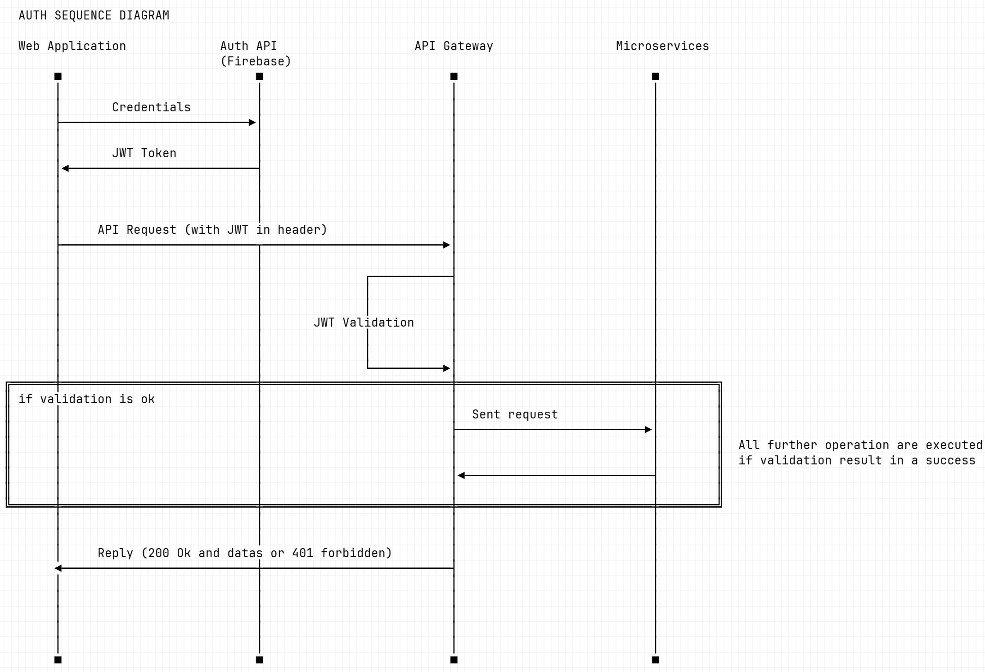
\includegraphics[width=\textwidth, height=\textheight, keepaspectratio]{auth.jpg}
  \caption{Sequence Diagram -- Flusso di Autenticazione}
  \label{fig:seq_auth}
\end{figure}

\newpage

\subsection{Aggiunta di un Alimento}

Il diagramma illustra la sequenza di operazioni per l'aggiunta di un nuovo alimento all'inventario. Dopo la verifica del token da parte del Gateway, la richiesta viene instradata al Fridge Service con i dati dell'alimento nel body. Il servizio verifica che l'utente sia effettivamente membro del frigorifero, costruisce il documento MongoDB arricchendolo con il campo \texttt{owner\_id} (recuperato dall'header \texttt{X-User-Id}), e lo persiste nella collection degli alimenti. La risposta include il documento creato con il relativo \texttt{\_id} generato da MongoDB.

\begin{figure}[H]
  \centering
  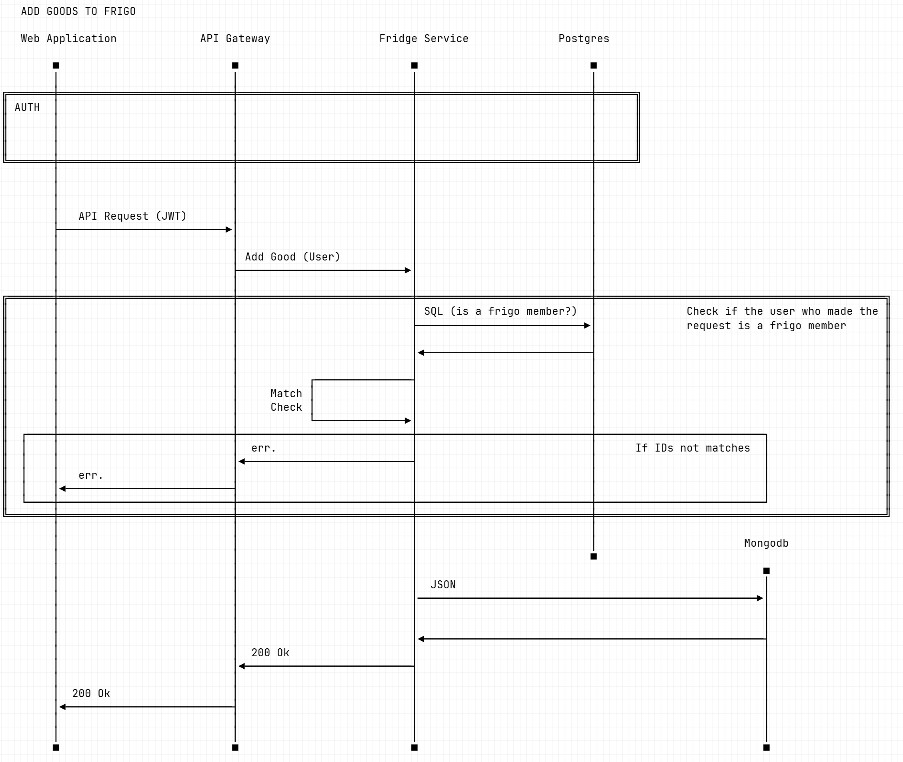
\includegraphics[width=\textwidth, height=\textheight, keepaspectratio]{add_goods.jpg}
  \caption{Sequence Diagram -- Aggiunta Alimento all'Inventario}
  \label{fig:seq_add}
\end{figure}

\newpage

\subsection{Creazione Frigorifero}

Il diagramma mostra come viene creato un nuovo frigorifero virtuale. Il Fridge Service esegue due operazioni distinte in sequenza: inserisce il record del frigorifero nella tabella \texttt{FRIDGES} di PostgreSQL, quindi aggiunge l'utente richiedente nella tabella \texttt{FRIDGE\_MEMBERS} con il ruolo \texttt{OWNER}. L'atomicità delle due operazioni garantisce che non possa esistere un frigorifero senza un proprietario associato. Il nuovo frigorifero è immediatamente visibile nella Dashboard dell'utente.

\begin{figure}[H]
  \centering
  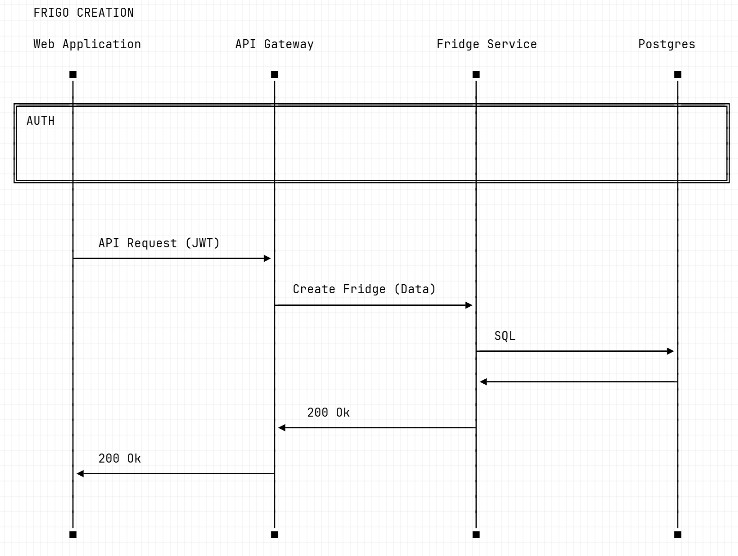
\includegraphics[width=\textwidth, height=\textheight, keepaspectratio]{creation_fridge.jpg}
  \caption{Sequence Diagram -- Creazione di un Nuovo Frigorifero}
  \label{fig:seq_create}
\end{figure}

\newpage

\subsection{Invito Utenti al Frigorifero}

Il diagramma descrive il meccanismo di invito basato su token temporanei. L'Admin del Frigo richiede la generazione di un link: il Fridge Service crea un token UUID, lo persiste in \texttt{FRIDGE\_INVITATIONS} con scadenza a 24 ore, e restituisce l'URL di invito al client. Quando un secondo utente accede al link, il sistema verifica la validità e la non-scadenza del token, aggiunge il nuovo utente come \texttt{MEMBER} in \texttt{FRIDGE\_MEMBERS}, e marca il token come utilizzato per impedirne il riuso.

\begin{figure}[H]
  \centering
  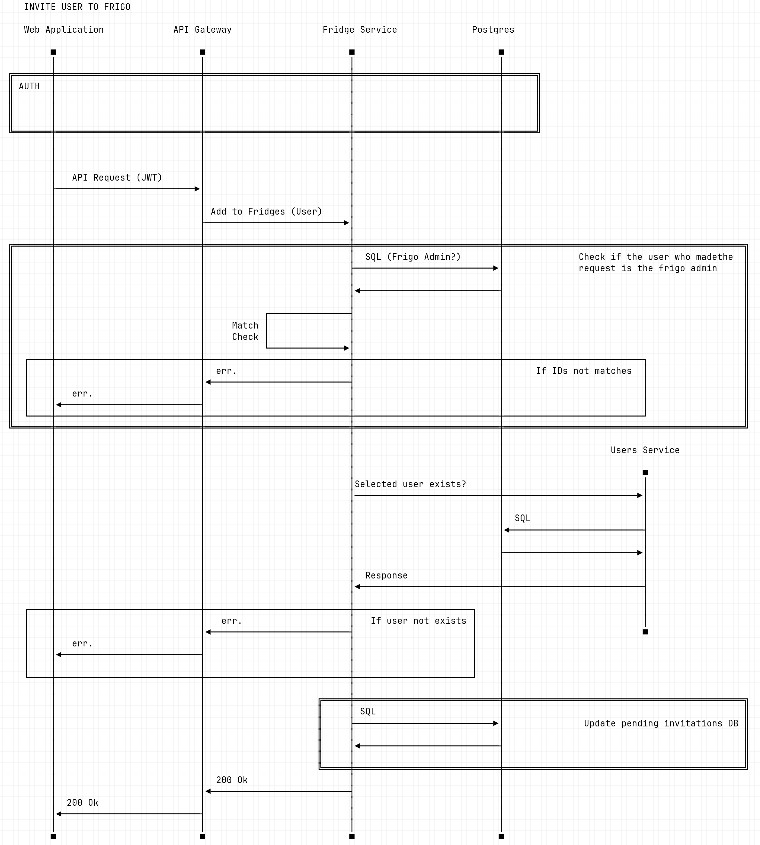
\includegraphics[width=\textwidth, height=\textheight, keepaspectratio]{invite_usr_fridge.jpg}
  \caption{Sequence Diagram -- Generazione e Accettazione Link di Invito}
  \label{fig:seq_invite}
\end{figure}

\newpage

\subsection{Gestione Frigorifero (Modifica e Cancellazione)}

Il diagramma illustra le operazioni di modifica del nome e cancellazione di un frigorifero, entrambe riservate all'utente con ruolo \texttt{OWNER}. Prima di eseguire qualsiasi operazione, il Fridge Service verifica il ruolo dell'utente tramite una query su \texttt{FRIDGE\_MEMBERS}; in caso di ruolo insufficiente risponde con \texttt{403 Forbidden}. La cancellazione è un'operazione a cascata: vengono eliminati in sequenza tutti gli alimenti in MongoDB, i record in \texttt{FRIDGE\_MEMBERS}, i token di invito in \texttt{FRIDGE\_INVITATIONS} e infine il record del frigorifero in \texttt{FRIDGES}.

\begin{figure}[H]
  \centering
  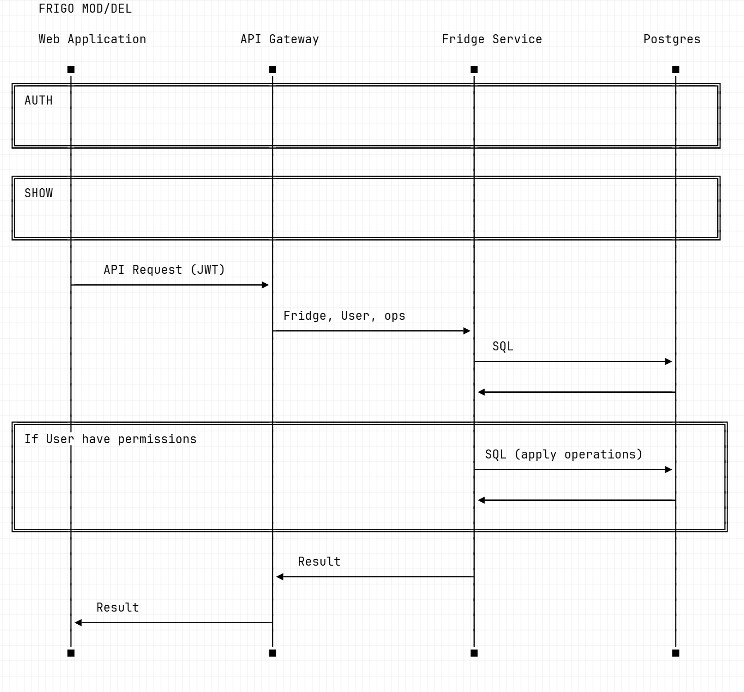
\includegraphics[width=\textwidth, height=\textheight, keepaspectratio]{mod_del_fridge.jpg}
  \caption{Sequence Diagram -- Modifica e Cancellazione del Frigorifero}
  \label{fig:seq_manage}
\end{figure}

\newpage

\subsection{Visualizzazione Alimenti del Frigorifero}

Il diagramma descrive il recupero dell'inventario di un frigorifero. Il Fridge Service esegue una query MongoDB filtrando per \texttt{fridge\_id}, e restituisce la lista dei documenti alimento. Il frontend riceve l'array e popola la vista inventario applicando, lato client, l'ordinamento selezionato dall'utente tramite la funzione \texttt{sortIngredients()} (UC9). L'operazione è in sola lettura e non modifica lo stato del sistema.

\begin{figure}[H]
  \centering
  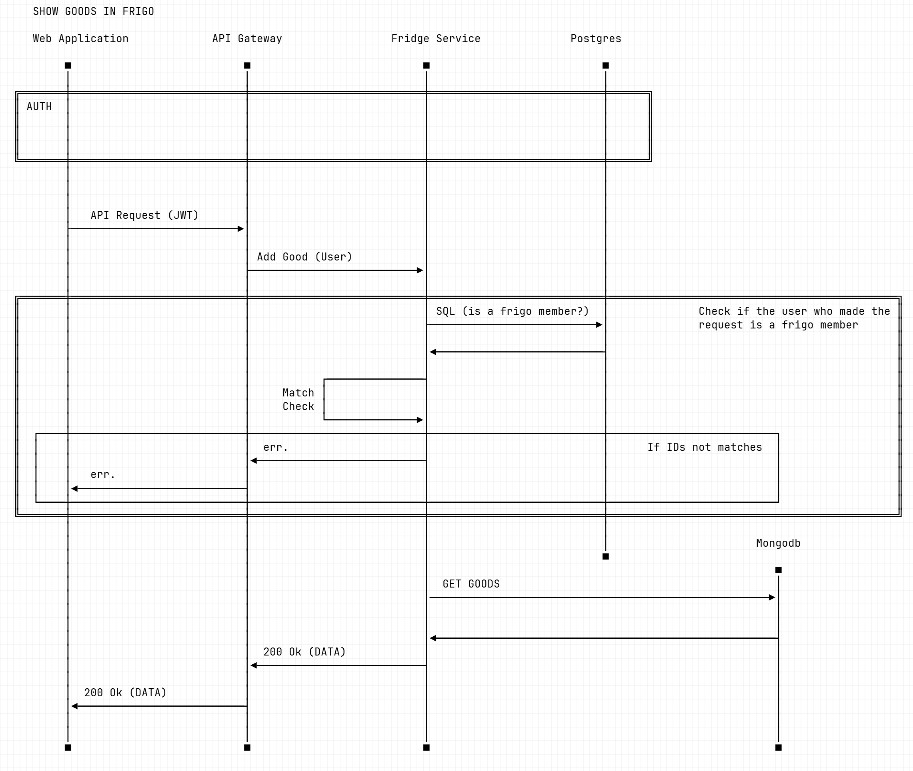
\includegraphics[width=\textwidth, height=\textheight, keepaspectratio]{show_goods.jpg}
  \caption{Sequence Diagram -- Recupero e Visualizzazione degli Alimenti}
  \label{fig:seq_items}
\end{figure}

\newpage

\subsection{Visualizzazione Lista Frigoriferi}

Il diagramma mostra come la Dashboard recupera i frigoriferi dell'utente autenticato. Il Fridge Service esegue una JOIN tra \texttt{FRIDGES} e \texttt{FRIDGE\_MEMBERS} filtrando per \texttt{user\_id}, e restituisce per ogni frigorifero il nome, la data di creazione e il ruolo dell'utente (\texttt{OWNER} o \texttt{MEMBER}). Questa informazione sul ruolo viene utilizzata dal frontend per mostrare o nascondere le azioni amministrative (modifica, cancellazione, gestione membri) nell'interfaccia utente.

\begin{figure}[H]
  \centering
  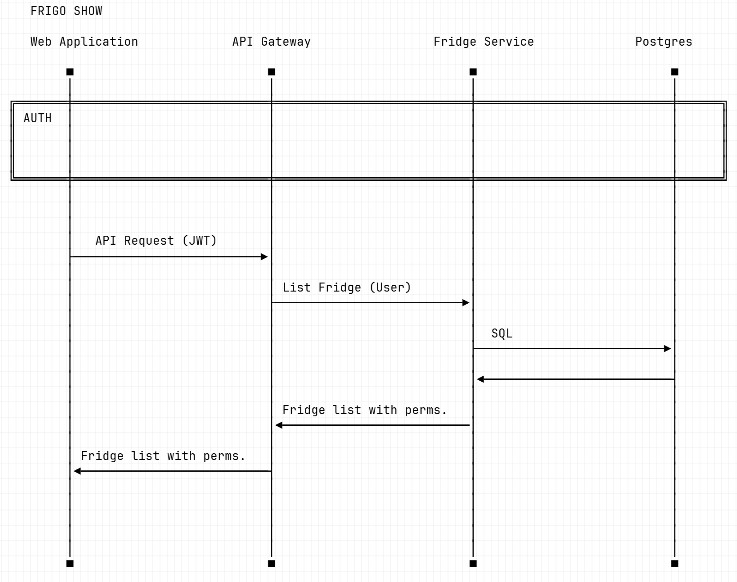
\includegraphics[width=\textwidth, height=\textheight, keepaspectratio]{show_fridge.jpg}
  \caption{Sequence Diagram -- Recupero e Visualizzazione dei Frigoriferi nella Dashboard}
  \label{fig:seq_fridges}
\end{figure}

\newpage
\section{UML Class Diagram -- Schema dei Dati}

Il \textbf{Class Diagram} viene qui utilizzato per rappresentare la struttura delle entità dati principali del sistema e le relazioni tra esse. Il modello è suddiviso in due schemi distinti in base alla tecnologia di persistenza:

\begin{itemize}
  \item \textbf{Schema SQL (PostgreSQL)}: per le entità con struttura fissa e relazioni forti, quali \texttt{Users}, \texttt{Fridges}, \texttt{FridgeMembers} e \texttt{FridgeInvitations}. Le chiavi esterne e i vincoli di unicità garantiscono l'integrità referenziale.
  \item \textbf{Schema NoSQL (MongoDB)}: per l'entità \texttt{Item}, che rappresenta un alimento nell'inventario. La natura eterogenea degli attributi degli alimenti (campo \texttt{brand} opzionale, \texttt{notes}, oggetto \texttt{sharing\_status} annidato) rende il documento MongoDB la struttura più adatta. Il modello flessibile facilita inoltre la trasmissione dell'intero documento all'LLM durante la generazione delle ricette, senza necessità di JOIN.
\end{itemize}

\begin{figure}[H]
  \centering
  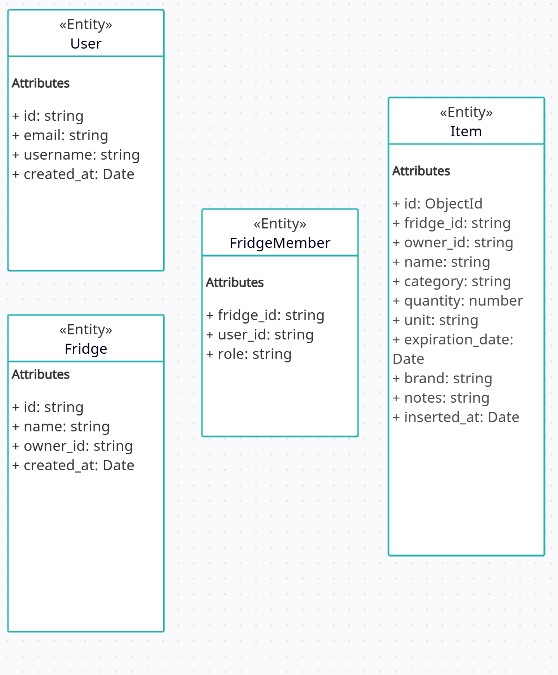
\includegraphics[width=0.7\textwidth]{Iteration_1_cd_data_type.jpg}
  \caption{Class Diagram -- Schema dei Tipi di Dato (SQL e NoSQL)}
  \label{fig:class}
\end{figure}

\section{Testing}

\subsection{Analisi Statica -- ESLint}

L'analisi statica è stata condotta tramite ESLint su tutti i servizi del progetto. I report evidenziano la conformità del codice alle regole definite nella configurazione, con indicazione delle eventuali violazioni per file e riga. Durante lo sviluppo dell'Iterazione 1 sono state risolte tutte le segnalazioni di livello \textit{error}, mentre alcune segnalazioni di livello \textit{warning} sono state accettate consapevolmente (es. uso di \texttt{console.log} per il debug).

\begin{figure}[H]
  \centering
  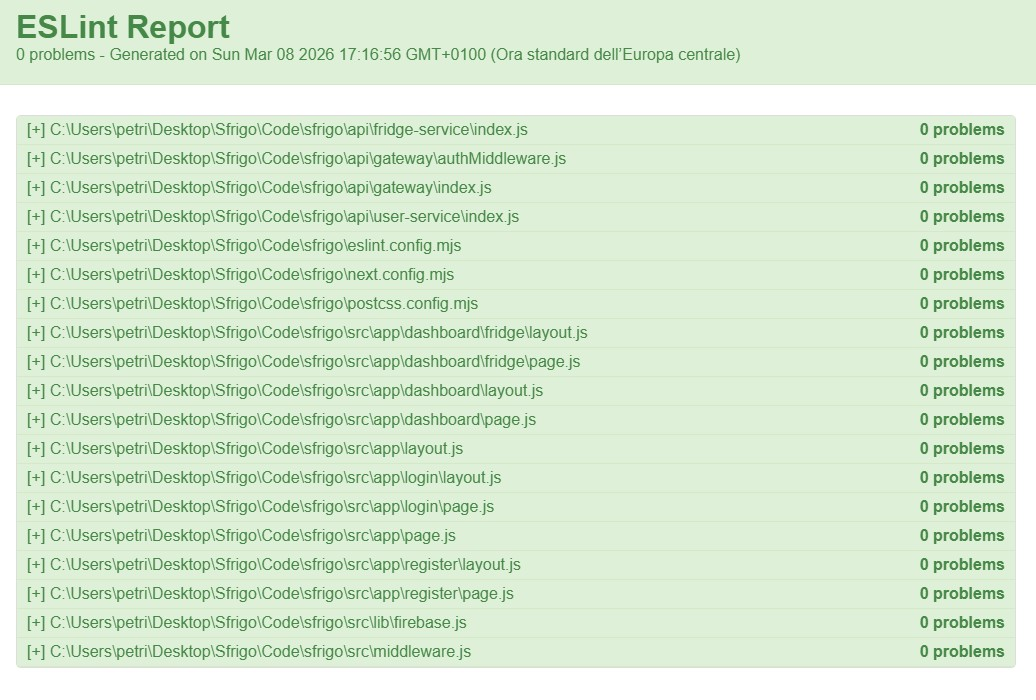
\includegraphics[width=\textwidth, height=\textheight, keepaspectratio]{Static_Analisis_Eslint.jpg}
  \caption{Report di Analisi Statica -- ESLint}
  \label{fig:eslint}
\end{figure}

\subsection{Analisi Dinamica -- Jest e Supertest}

Per eseguire l'analisi dinamica sono stati scelti \textbf{Jest} e \textbf{Supertest}.

\textbf{Jest} è un framework di testing per JavaScript sviluppato da Meta, scelto per la sua facile integrazione con progetti Node.js e Next.js, il sistema di mock integrato che permette di simulare dipendenze esterne (come database e servizi), la generazione automatica dei report di coverage e la configurazione minima, che riconosce automaticamente i file di test nella cartella \texttt{\_\_tests\_\_/}.

\textbf{Supertest} è una libreria utilizzata per testare applicazioni HTTP Express senza avviare un server reale. Permette di simulare richieste GET, POST e DELETE direttamente in memoria ed è facilmente integrabile con Jest per verificare le risposte delle API in modo semplice e rapido.

Di seguito è riportato un esempio di test relativo al \texttt{user-service}:

\begin{lstlisting}[language=java, caption={Test UC -- user-service}]
const request = require('supertest');

// Mock del database pg prima di importare il servizio
jest.mock('pg', () => {
  const mPool = {
    query: jest.fn()
  };
  return { Pool: jest.fn(() => mPool) };
});

const { Pool } = require('pg');
const pool = new Pool();

// Importo app
const app = require('../api/user-service/index.js');

describe('User Service - POST /users', () => {

  beforeEach(() => {
    jest.clearAllMocks(); // resetta i mock prima di ogni test
  });

  test('TC-US-001 - Ritorna 401 se mancano gli header', async () => {
    const res = await request(app)
      .post('/users')
      .send({ username: 'testuser' });
    expect(res.status).toBe(401);
  });

  test('TC-US-002 - Ritorna 400 se manca username', async () => {
    const res = await request(app)
      .post('/users')
      .set('X-User-Id', 'firebase-uid-123')
      .set('X-User-Email', 'test@test.com')
      .send({});
    expect(res.status).toBe(400);
  });

  test('TC-US-003 - Ritorna 201 se tutto ok', async () => {
    pool.query.mockResolvedValueOnce({
      rows: [{
        id: 'firebase-uid-123',
        username: 'testuser',
        email: 'test@test.com',
        created_at: new Date()
      }]
    });
    const res = await request(app)
      .post('/users')
      .set('X-User-Id', 'firebase-uid-123')
      .set('X-User-Email', 'test@test.com')
      .send({ username: 'testuser' });
    expect(res.status).toBe(201);
    expect(res.body.username).toBe('testuser');
  });

});
\end{lstlisting}

\begin{figure}[H]
  \centering
  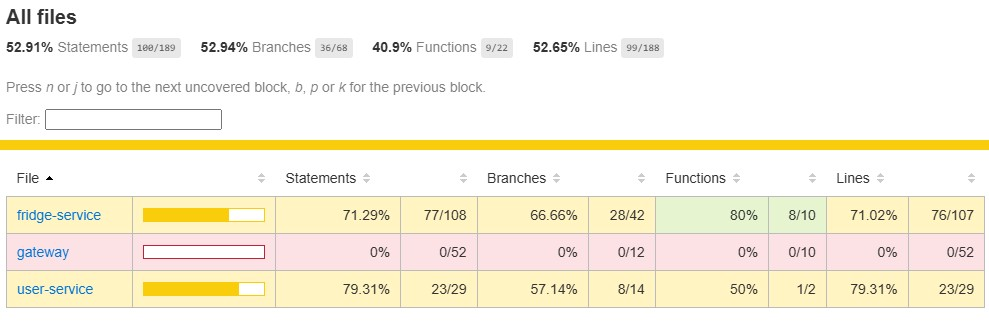
\includegraphics[width=\textwidth, height=\textheight, keepaspectratio]{Dynamic_Analisis_Coverage_jest.jpg}
  \caption{Report di Coverage -- Jest (Iterazione 1)}
  \label{fig:coverage}
\end{figure}

\textit{Disclaimer:} Il Gateway utilizza Firebase Admin SDK per la validazione dei token JWT. Poiché Firebase Authentication non è eseguibile in locale come un normale database, il mock dell'SDK richiederebbe la simulazione dell'intera infrastruttura di autenticazione Google. Per questo motivo il testing del Gateway è stato effettuato manualmente tramite \textbf{Postman}, inviando token Firebase reali ottenuti dopo un'autenticazione effettiva. Questo approccio garantisce la verifica del comportamento reale del servizio, a differenza di un mock che potrebbe mascherare problemi di integrazione.

\section{Documentazione API}

Le API sviluppate nell'Iterazione 1 sono state verificate manualmente tramite Postman. Per ogni endpoint vengono riportati il metodo HTTP, il percorso, i parametri principali e la risposta restituita dal sistema.

\subsection{Add Item e Delete Item}

\texttt{POST /api/v1/fridges/:fridgeId/items} aggiunge un nuovo alimento all'inventario del frigorifero specificato. Il body JSON deve includere almeno \texttt{name}, \texttt{category}, \texttt{quantity} e \texttt{unit}; il campo \texttt{owner\_id} viene iniettato automaticamente dal Fridge Service tramite l'header \texttt{X-User-Id}. In caso di successo restituisce \texttt{201 Created} con il documento MongoDB creato.

\texttt{DELETE /api/v1/fridges/:fridgeId/items/:itemId} rimuove l'alimento identificato da \texttt{itemId} dall'inventario. Il servizio verifica che l'utente richiedente sia il proprietario dell'alimento o abbia ruolo OWNER nel frigorifero prima di procedere con la cancellazione; in caso contrario risponde con \texttt{403 Forbidden}.

\begin{figure}[H]
  \centering
  \begin{minipage}[t]{0.48\textwidth}
    \centering
    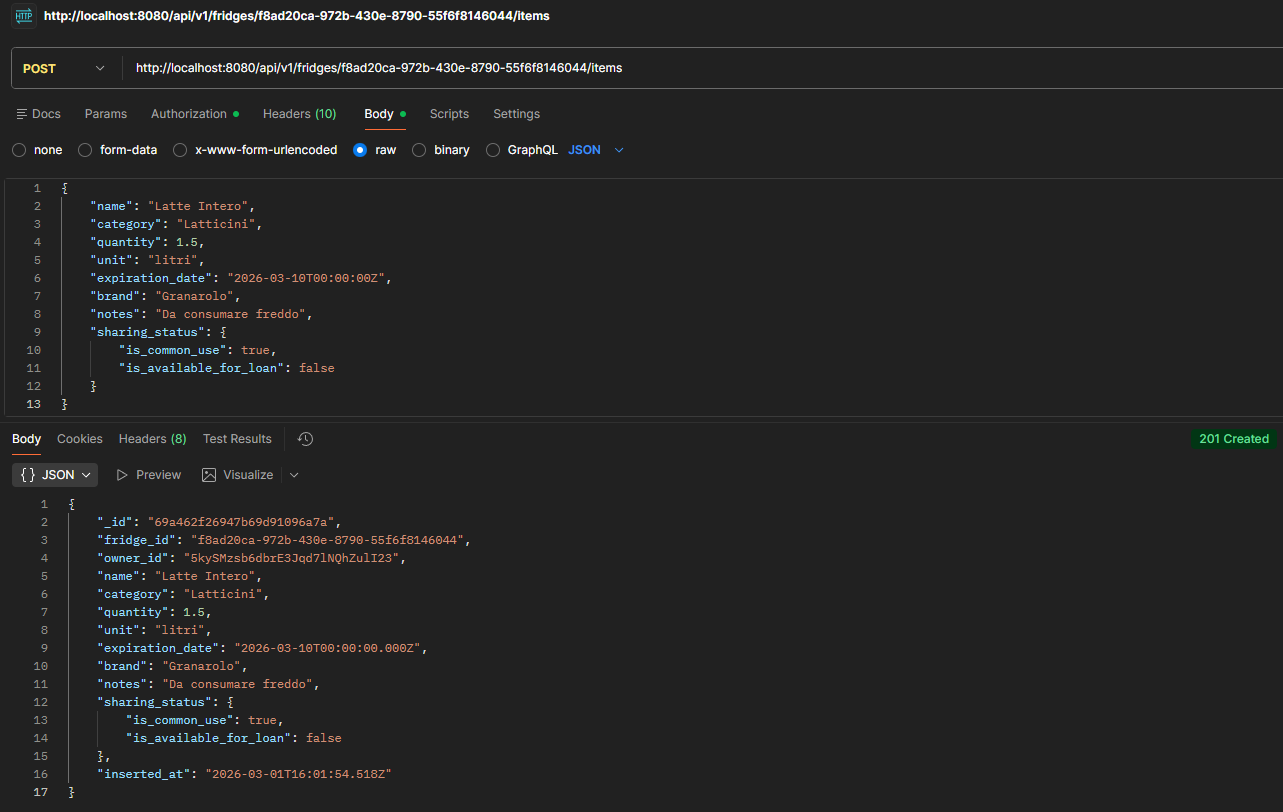
\includegraphics[width=\linewidth, height=0.28\textheight, keepaspectratio]{add-item.png}
    \caption{POST /api/v1/fridges/:id/items}
    \label{fig:api_add}
  \end{minipage}
  \hfill
  \begin{minipage}[t]{0.48\textwidth}
    \centering
    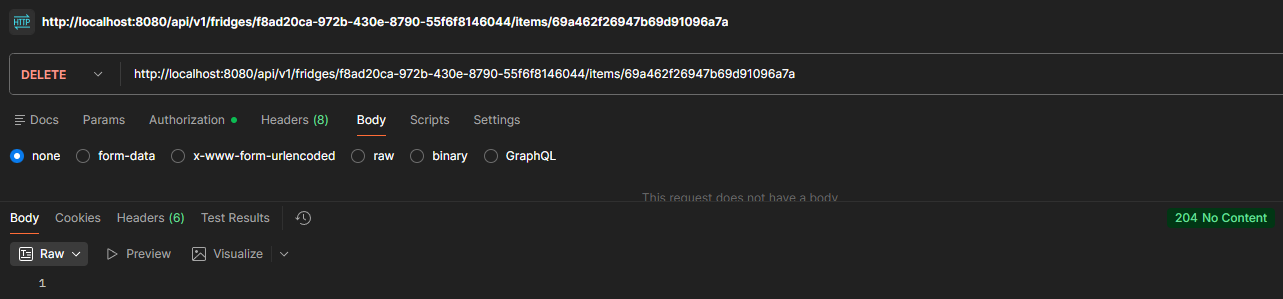
\includegraphics[width=\linewidth, height=0.28\textheight, keepaspectratio]{delete-item.png}
    \caption{DELETE /api/v1/fridges/:id/items/:itemId}
    \label{fig:api_delete}
  \end{minipage}
\end{figure}

\subsection{Get Frigos e Get Items}

\texttt{GET /api/v1/fridges} restituisce la lista dei frigoriferi a cui l'utente autenticato appartiene, con indicazione del ruolo (\texttt{OWNER} o \texttt{MEMBER}) e della data di creazione. Il Fridge Service esegue una JOIN tra le tabelle \texttt{FRIDGES} e \texttt{FRIDGE\_MEMBERS} filtrando per \texttt{user\_id}.

\texttt{GET /api/v1/fridges/:fridgeId/items} restituisce l'inventario completo del frigorifero. Prima di eseguire la query MongoDB, il servizio verifica che l'utente sia membro del frigorifero tramite la tabella \texttt{FRIDGE\_MEMBERS}; in caso contrario risponde \texttt{403 Forbidden}. La risposta è un array di documenti alimento ordinati per data di inserimento.

\begin{figure}[H]
  \centering
  \begin{minipage}[t]{0.48\textwidth}
    \centering
    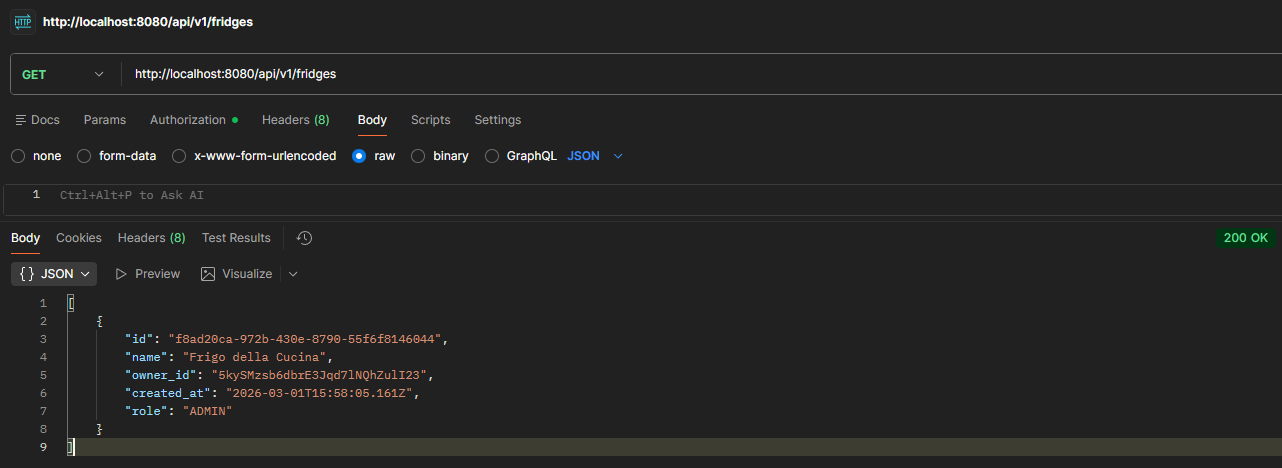
\includegraphics[width=\linewidth, height=0.28\textheight, keepaspectratio]{get-frigos.png}
    \caption{GET /api/v1/fridges}
    \label{fig:api_frigos}
  \end{minipage}
  \hfill
  \begin{minipage}[t]{0.48\textwidth}
    \centering
    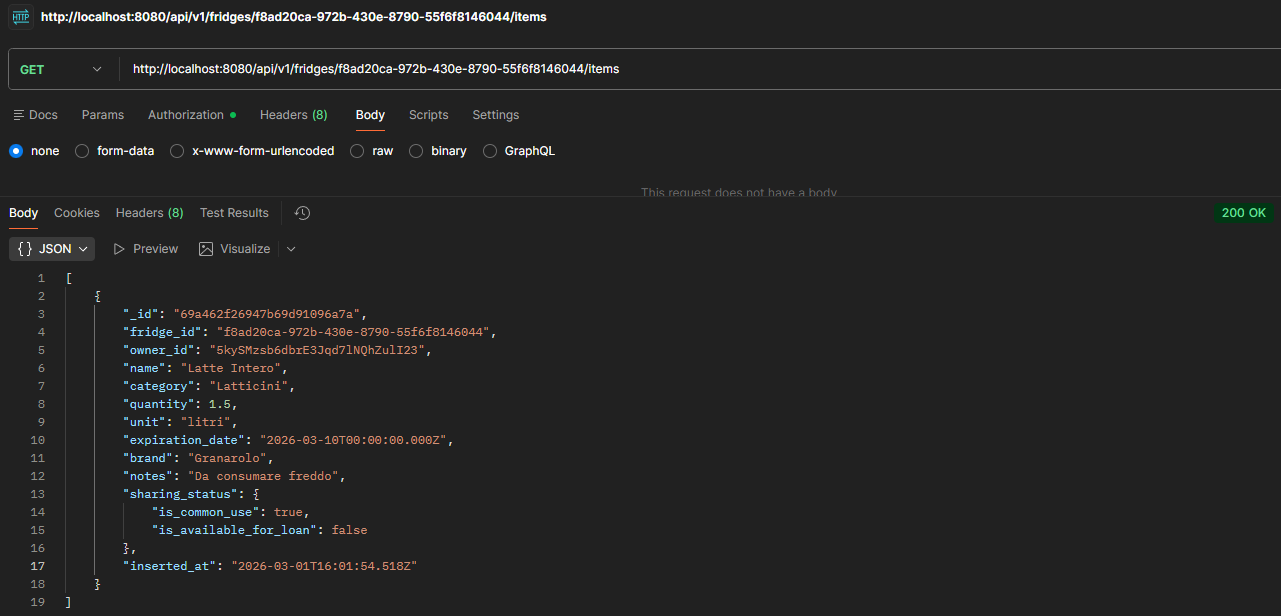
\includegraphics[width=\linewidth, height=0.28\textheight, keepaspectratio]{get-items.png}
    \caption{GET /api/v1/fridges/:id/items}
    \label{fig:api_items}
  \end{minipage}
\end{figure}

\subsection{Login tramite Firebase}

Il login non è gestito da un endpoint REST applicativo, ma direttamente dall'SDK Firebase lato client. Dopo l'autenticazione con email/password o provider Google, Firebase rilascia un token JWT che il frontend allega in ogni richiesta nell'header \texttt{Authorization: Bearer <token>}. Il Gateway lo verifica tramite Firebase Admin SDK e, se valido, estrae \texttt{uid} e \texttt{email} dell'utente per propagarli ai microservizi. Lo screenshot mostra il token JWT ottenuto e la risposta del Gateway a una richiesta autenticata, confermando che la catena di verifica funziona correttamente end-to-end.

\begin{figure}[H]
  \centering
  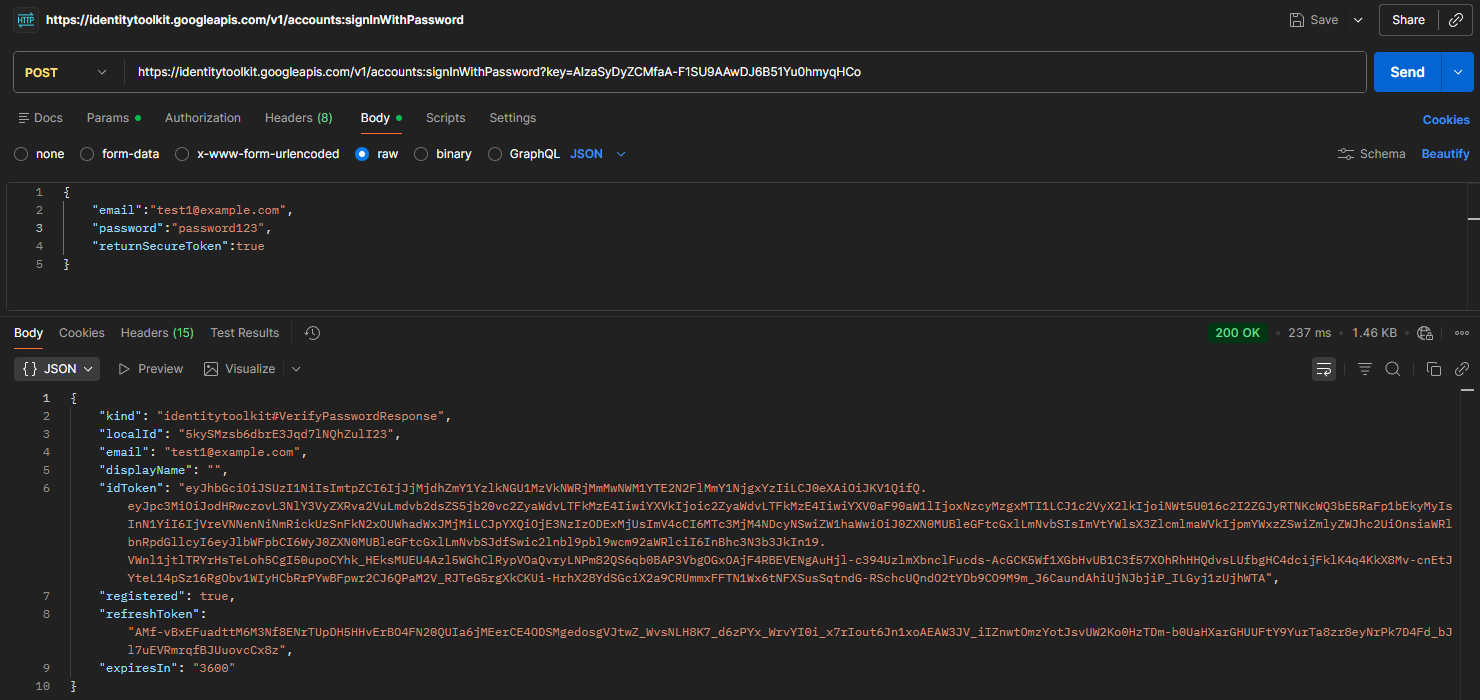
\includegraphics[width=0.75\textwidth, height=0.32\textheight, keepaspectratio]{login-firebase.png}
  \caption{Verifica del token Firebase tramite Gateway}
  \label{fig:api_login}
\end{figure}

% ============================================================
\chapter{Iterazione 2}

\section{Introduzione}

Con il nucleo funzionale completato nell'Iterazione 1, la seconda iterazione si concentra sulle funzionalità collaborative avanzate che costituiscono il valore differenziale di Sfrigo rispetto a una semplice lista della spesa condivisa. I work item selezionati per questo sprint sono tutti i casi d'uso di media priorità, raggruppabili in tre aree tematiche strettamente interconnesse.

La prima area riguarda la \textbf{gestione della condivisione}: UC5 introduce il concetto di alimento di uso comune, mentre UC6 garantisce che ogni alimento sia sempre tracciato al proprio proprietario. Questi due work item sono propedeutici agli algoritmi dei punti successivi, poiché senza la distinzione proprietario/comune non sarebbe possibile calcolare contributi equi né separare ricette personali da condivise.

La seconda area riguarda la \textbf{generazione di ricette tramite AI}: UC7 e UC8 implementano rispettivamente la ricetta personale (solo ingredienti dell'utente) e quella condivisa (ingredienti comuni del gruppo). Entrambi si appoggiano al Recipe Service introdotto nell'architettura ma non ancora attivato nell'Iterazione 1. UC9 completa questa area con l'algoritmo di sorting dell'inventario, che permette di ordinare gli alimenti per urgenza di consumo e quindi di orientare la scelta degli ingredienti da utilizzare per primi.

La terza area riguarda la \textbf{gestione avanzata dei membri}: UC10 introduce l'algoritmo di equità che calcola il contributo di ciascun membro al frigorifero condiviso, UC11 consente a un utente di abbandonare volontariamente un frigorifero, e UC12 permette all'Admin di rimuovere un membro. In questa iterazione viene inoltre integrata la pipeline \textbf{CI/CD} tramite GitHub Actions, automatizzando il ciclo di test, build e pubblicazione delle immagini Docker ad ogni push sul branch \texttt{main}.

\begin{center}
\begin{tabular}{@{} l l l @{}}
  \toprule
  \textbf{Caso d'uso} & \textbf{Funzionalità} & \textbf{Area} \\
  \midrule
  UC5   & Alimento di Uso Comune             & Condivisione \\
  UC6   & Tracciamento Proprietario Alimento & Condivisione \\
  UC7   & Richiesta Ricetta Personale        & Ricette AI \\
  UC8   & Richiesta Ricetta Condivisa        & Ricette AI \\
  UC9   & Algoritmo di Sorting               & Ricette AI \\
  UC10  & Algoritmo di Equità               & Gestione membri \\
  UC11  & Uscita Volontaria dal Frigorifero  & Gestione membri \\
  UC12  & Rimozione Utente dal Frigorifero   & Gestione membri \\
  \bottomrule
\end{tabular}
\end{center}

\section{Descrizione dei Casi d'Uso}

\subsection{UC5 -- Alimento di Uso Comune}

\begin{ucbox}
\textbf{Descrizione:} Durante l'inserimento di un alimento, l'utente può marcarlo come \textit{di uso comune}, rendendolo disponibile a tutti i membri del frigorifero per la generazione di ricette condivise. Lo stato di condivisione è memorizzato nel campo \texttt{sharing\_status.is\_common\_use} del documento MongoDB.

\begin{description}[leftmargin=4cm, style=sameline]
  \item[Attori Coinvolti:] Utente membro del frigorifero
  \item[Precondizione:] Utente loggato; form di aggiunta alimento aperto
  \item[Postcondizione:] Alimento salvato con flag \texttt{is\_common\_use: true}
  \item[Trigger:] L'utente spunta la casella \textit{``Alimento Condiviso''} durante l'aggiunta
\end{description}
\end{ucbox}

\textbf{Svolgimento standard:}
\begin{enumerate}
  \item L'utente segue il flusso di UC3.1 -- Aggiungi Alimento.
  \item L'utente spunta la casella \textit{``Alimento Condiviso''} nel form.
  \item Il sistema salva l'alimento con \texttt{is\_common\_use: true} in MongoDB.
  \item L'alimento è ora selezionabile da tutti i membri nelle ricette condivise.
\end{enumerate}

\newpage
\subsection{UC6 -- Tracciamento Proprietario Alimento}

\begin{ucbox}
\textbf{Descrizione:} Ad ogni alimento aggiunto viene automaticamente associato il campo \texttt{owner\_id} con l'identificativo dell'utente che lo ha inserito. Questo avviene in modo trasparente senza richiedere interazioni aggiuntive. Il tracciamento del proprietario è fondamentale per l'algoritmo di equità e per il controllo degli accessi in fase di eliminazione.

\begin{description}[leftmargin=4cm, style=sameline]
  \item[Attori Coinvolti:] Utente membro del frigorifero (implicitamente)
  \item[Precondizione:] Utente loggato
  \item[Postcondizione:] Il documento MongoDB dell'alimento contiene \texttt{owner\_id} con l'UID dell'utente corrente
  \item[Trigger:] L'utente esegue UC3.1 -- Aggiungi Alimento
\end{description}
\end{ucbox}

\newpage
\subsection{UC7 -- Richiesta Ricetta Personale}

\begin{ucbox}
\textbf{Descrizione:} L'utente loggato accede all'inventario di un frigorifero e richiede una ricetta personale tramite il servizio AI. Il sistema genera ricette basandosi sugli ingredienti selezionati dall'utente utilizzando l'API OpenAI. La ricetta viene preparata considerando solo gli ingredienti scelti dall'utente, che al termine vengono rimossi dall'inventario.

\begin{description}[leftmargin=4cm, style=sameline]
  \item[Attori Coinvolti:] Utente membro del frigorifero
  \item[Precondizione:] Utente loggato; almeno 2 alimenti personali nell'inventario
  \item[Postcondizione:] Ricette generate dall'LLM mostrate all'utente; ingredienti selezionati rimossi al momento della scelta
  \item[Trigger:] Clic sul pulsante \textit{``Ricetta AI''} $\to$ selezione \textit{``Ricetta Personale''}
\end{description}
\end{ucbox}

\textbf{Svolgimento standard:}
\begin{enumerate}
  \item L'utente loggato accede all'inventario del frigo.
  \item L'utente clicca il bottone \textit{``Ricetta AI''}.
  \item Il sistema mostra le opzioni disponibili: \textit{``Ricetta Personale''} e \textit{``Ricetta Condivisa''}.
  \item L'utente clicca su \textit{``Ricetta Personale''}.
  \item Il sistema mostra gli ingredienti selezionabili dall'inventario.
  \item L'utente seleziona almeno 2 ingredienti.
  \item L'utente clicca su \textit{``Cerca Ricette''}.
  \item Il sistema invia la richiesta all'API OpenAI e genera una lista di ricette suggerite.
  \item L'utente visualizza le ricette proposte e sceglie quella desiderata.
  \item L'utente clicca su \textit{``Usa questa ricetta''}.
  \item Il sistema rimuove dall'inventario gli ingredienti selezionati.
\end{enumerate}


\newpage
\subsection{UC8 -- Richiesta Ricetta Condivisa}

\begin{ucbox}
\textbf{Descrizione:} L'utente loggato accede all'inventario di un frigorifero condiviso e richiede una ricetta condivisa tramite il servizio AI. A differenza della ricetta personale, la ricetta condivisa considera l'intero inventario del frigo, accessibile da tutti i membri. Gli ingredienti selezionati vengono rimossi dall'inventario al termine.

\begin{description}[leftmargin=4cm, style=sameline]
  \item[Attori Coinvolti:] Utente membro del frigorifero
  \item[Precondizione:] Utente loggato; almeno 2 alimenti comuni presenti nell'inventario
  \item[Postcondizione:] Ricette generate basate sugli alimenti condivisi; ingredienti rimossi con aggiornamento del bilancio di equità
  \item[Trigger:] Clic sul pulsante \textit{``Ricetta AI''} $\to$ selezione \textit{``Ricetta Condivisa''}
\end{description}
\end{ucbox}

\textbf{Svolgimento standard:}
\begin{enumerate}
  \item L'utente loggato accede all'inventario del frigo.
  \item L'utente clicca il bottone \textit{``Ricetta AI''}.
  \item Il sistema mostra le opzioni disponibili: \textit{``Ricetta Personale''} e \textit{``Ricetta Condivisa''}.
  \item L'utente clicca su \textit{``Ricetta Condivisa''}.
  \item Il sistema mostra gli ingredienti selezionabili dall'inventario condiviso.
  \item L'utente seleziona almeno 2 ingredienti.
  \item L'utente clicca su \textit{``Cerca Ricette''}.
  \item Il sistema invia la richiesta all'API OpenAI e genera una lista di ricette suggerite.
  \item L'utente visualizza le ricette proposte e sceglie quella desiderata.
  \item L'utente clicca su \textit{``Usa questa ricetta''}.
  \item Il sistema rimuove dall'inventario condiviso gli ingredienti selezionati.
\end{enumerate}

\newpage
\subsection{UC9 -- Algoritmo di Sorting}

\begin{ucbox}
\textbf{Descrizione:}Il sistema ordina e prioritizza gli alimenti nell'inventario tramite una funzione di sorting che supporta più modalità. La modalità più sofisticata è \textit{urgency}, che implementa un algoritmo di ordinamento basato su uno score composito.

\begin{description}[leftmargin=4cm, style=sameline]
  \item[Attori Coinvolti:] Utente membro del frigorifero
  \item[Precondizione:] Utente loggato; inventario non vuoto
  \item[Postcondizione:] Alimenti visualizzati ordinati secondo il criterio selezionato
  \item[Trigger:] Selezione di una modalità di ordinamento nel menu dell'inventario
\end{description}
\end{ucbox}

\textbf{Modalità di ordinamento disponibili:}
\begin{itemize}
  \item \textbf{Nome} (A$\rightarrow$Z, Z$\rightarrow$A): ordinamento alfabetico.
  \item \textbf{Scadenza}: dall'alimento con scadenza più imminente al più lontano.
  \item \textbf{Categoria}: raggruppamento per categoria alimentare.
  \item \textbf{Proprietario}: raggruppamento per utente proprietario.
  \item \textbf{Urgenza}: score composito basato su scadenza, categoria e quantità residua.
\end{itemize}

\textbf{Pseudocodice -- MergeSort con \texttt{compareFn}:}

\begin{lstlisting}[language=java, caption={Algoritmo di Sorting -- MergeSort}]
sort(compareFn)
  MergeSort(list, left, right)
    if left >= right -> return
    middle = (left + right) / 2
    MergeSort(list, left, middle)
    MergeSort(list, middle + 1, right)
    Merge(list, left, middle, right)

Merge(list, left, middle, right)
  // Confronto tramite compareFn(a, b)
  while i < n1 && j < n2
    if compareFn(leftArray[i], rightArray[j]) <= 0
      list[k] = leftArray[i]; i++
    else
      list[k] = rightArray[j]; j++
    k++
\end{lstlisting}

\textbf{Complessità:}
\begin{itemize}
  \item Ricorsione e divisione: $O(\log_2 n)$
  \item Merge: $O(n)$
  \item \textbf{Totale: $O(n \log n)$}
\end{itemize}

Per la modalità \textit{urgency} è stato adottato uno \textbf{score composito}: il 70\% del peso è dato da uno score di scadenza e il 30\% dalla categoria dell'alimento. La funzione \texttt{clamp} mantiene i valori tra 0 e 30, normalizzandoli successivamente:

\begin{equation}
  \text{score} = (\text{expiryScore} \times 0.7) + ((1 - \text{categoryWeight}) \times 0.3)
\end{equation}
\begin{equation}
  \text{expiryScore} = \frac{\text{clamp}(\text{daysUntilExpiry},\ 0,\ 30)}{30}
\end{equation}

\newpage
\subsection{UC10 -- Algoritmo di Equità}

\begin{ucbox}
\textbf{Descrizione:} Il sistema calcola e visualizza la distribuzione equa del contributo alimentare tra i membri del frigorifero condiviso. L'algoritmo considera il valore (stimato o effettivo) degli alimenti inseriti da ciascun utente e calcola quante risorse ciascun membro ha messo a disposizione della collettività, esprimendo il risultato in termini monetari o percentuali.

\begin{description}[leftmargin=4cm, style=sameline]
  \item[Attori Coinvolti:] Utente membro del frigorifero
  \item[Precondizione:] Frigorifero con almeno 2 membri; alimenti presenti nell'inventario condiviso
  \item[Postcondizione:] Visualizzazione del riepilogo contributivo per ogni membro
  \item[Trigger:] Richiesta ricetta condivisa o accesso alla sezione \textit{``Equità''}
\end{description}
\end{ucbox}

\textbf{Pseudocodice -- Calcolo dell'Equità:}

\begin{lstlisting}[language=java, caption={Algoritmo di Equità -- GET /fridges/:fridgeId/equity}]
GET /fridges/:fridgeId/equity

  // Verifica accesso
  membership = checkFridgeMembership(fridgeId, userId)
  if !membership -> return 403

  // Recupera dati
  members = query PostgreSQL -> fridge_members JOIN users WHERE fridge_id
  recipes = query MongoDB   -> recipes WHERE fridge_id

  // Inizializza struttura stats
  for each member m in members:
    stats[m.user_id] = {
      recipes_participated: 0,   // R_u
      ingredients_provided: 0,   // C_u
      total_ingredients: 0,      // T_u
      members_per_recipe: []
    }

  // Calcola statistiche per ogni ricetta
  for each recipe in recipes:                       // O(r)
    snapshot    = recipe.members_snapshot
    ingredients = recipe.ingredients
    memberCount = len(snapshot)
    totalIngr   = len(ingredients)

    for each member in snapshot:                    // O(m)
      if member not in stats -> skip
      stats[member].recipes_participated += 1
      stats[member].total_ingredients    += totalIngr
      stats[member].members_per_recipe.push(memberCount)

      provided = count ingredients where owner_id == member  // O(i)
      stats[member].ingredients_provided += provided

  // Calcola equity index per ogni membro
  for each user u in stats:                         // O(u)
    R = recipes_participated
    C = ingredients_provided
    T = total_ingredients

    if R == 0:
      label = "Nessuna partecipazione"; confidence = 0
      continue

    contribution_rate = C / T
    expected_rate     = sum(1/n for n in members_per_recipe) / R
    equity_index      = contribution_rate / expected_rate
    confidence        = 1 - e^(-R/3)
    display_score     = equity_index * confidence

    // Assegna etichetta
    if display_score >= 1.1 -> "Contribuisce troppo"    (lightblue)
    if display_score >= 0.9 -> "In equilibrio"          (green)
    if display_score >= 0.6 -> "Contribuisce poco"      (yellow)
    if display_score >= 0.3 -> "Contribuisce raramente" (orange)
    else                    -> "Non contribuisce"       (red)

  // Ordina per display_score decrescente
  result.sort((a, b) -> b.display_score - a.display_score)  // O(u log u)

  return result
\end{lstlisting}

\newpage
L'endpoint \texttt{GET /api/v1/fridges/:fridgeId/equity} restituisce il calcolo aggiornato in tempo reale, permettendo ai membri di visualizzare lo stato dei contributi e di bilanciare le future aggiunte di alimenti.
\\

\textbf{Complessità:} il termine dominante è $O(r \cdot m \cdot i)$, corrispondente al loop più annidato. Considerando che un frigorifero difficilmente avrà un numero elevato di membri e ingredienti (es.\ $m = 10$, $i = 20$), si ottiene:
\[
  O(r \cdot m \cdot i) \approx O(r \times 10 \times 20) \approx O(r)
\]
La \textbf{complessità totale} dell'algoritmo è quindi $O(r)$.

\newpage
\subsection{UC11 -- Uscita Volontaria dal Frigorifero}

\begin{ucbox}
\textbf{Descrizione:} Un utente membro (non OWNER) può scegliere di abbandonare volontariamente un frigorifero. Al momento dell'uscita, il sistema può richiedere come gestire gli alimenti di proprietà dell'utente (rimuoverli o trasferirli all'OWNER).

\begin{description}[leftmargin=4cm, style=sameline]
  \item[Attori Coinvolti:] Utente membro (ruolo MEMBER)
  \item[Precondizione:] Utente loggato; membro del frigorifero con ruolo MEMBER
  \item[Postcondizione:] Utente rimosso da \texttt{FRIDGE\_MEMBERS}; alimenti dell'utente gestiti secondo la scelta
  \item[Trigger:] Clic sul pulsante \textit{``Lascia Frigorifero''} nelle impostazioni del frigo
\end{description}
\end{ucbox}

\subsection{UC12 -- Rimozione Utente dal Frigorifero}

\begin{ucbox}
\textbf{Descrizione:} L'Admin del Frigo (OWNER) può rimuovere un membro dal frigorifero. L'operazione è irreversibile e rimuove il record corrispondente dalla tabella \texttt{FRIDGE\_MEMBERS}.

\begin{description}[leftmargin=4cm, style=sameline]
  \item[Attori Coinvolti:] Admin del Frigo (ruolo OWNER)
  \item[Precondizione:] Utente loggato con ruolo OWNER; membro target presente nel frigorifero
  \item[Postcondizione:] Membro rimosso da \texttt{FRIDGE\_MEMBERS}; il membro espulso non ha più accesso al frigorifero
  \item[Trigger:] Clic sul pulsante \textit{``Rimuovi Membro''} nella gestione dei membri del frigo
\end{description}
\end{ucbox}

\newpage
\section{Sequence Diagram -- Iterazione 2}

I tre sequence diagram di questa iterazione coprono le funzionalità introdotte nei work item di media priorità. A differenza dei diagrammi dell'Iterazione 1, dove i flussi erano prevalentemente CRUD su entità singole, qui le interazioni coinvolgono più sorgenti dati (PostgreSQL e MongoDB in lettura combinata) e servizi esterni (OpenAI API), rendendo i flussi strutturalmente più complessi.

\subsection{Generazione Ricetta}

Il diagramma illustra il flusso completo della generazione ricetta, comune sia alla modalità personale (UC7) sia a quella condivisa (UC8). L'utente seleziona gli ingredienti desiderati nell'inventario e avvia la richiesta. Il Fridge Service recupera i documenti MongoDB degli ingredienti selezionati e li trasmette al Recipe Service. Quest'ultimo costruisce un prompt strutturato contenente i dati degli ingredienti (nome, categoria, quantità, unità) e lo invia all'API OpenAI GPT-4o-mini tramite una richiesta HTTP POST. L'LLM restituisce un array di ricette in formato JSON; il Recipe Service deserializza la risposta e la restituisce al frontend, che le mostra all'utente. Alla selezione della ricetta da parte dell'utente, il Fridge Service rimuove da MongoDB gli ingredienti utilizzati.

\begin{figure}[H]
  \centering
  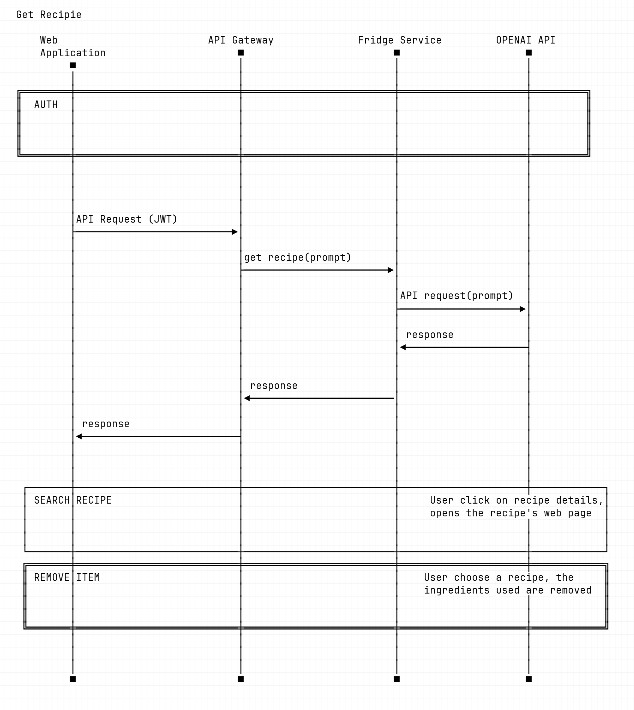
\includegraphics[width=0.6\textwidth]{get_recipe.jpg}
  \caption{Sequence Diagram -- Generazione Ricetta tramite LLM (UC7, UC8)}
  \label{fig:seq_recipe}
\end{figure}

\newpage

\subsection{Calcolo Equità}

Il diagramma descrive il flusso del calcolo dell'equità (UC10). Alla richiesta \texttt{GET /api/v1/fridges/:fridgeId/equity}, il Fridge Service esegue in parallelo due query: una su PostgreSQL per ottenere la lista dei membri del frigorifero con i rispettivi identificativi, e una su MongoDB per recuperare tutti gli alimenti comuni (\texttt{is\_common\_use: true}) con il loro valore stimato. Con questi dati, il servizio aggrega il contributo totale per \texttt{owner\_id}, calcola la quota ideale per membro (valore totale / numero di membri) e restituisce per ciascun utente il delta rispetto alla quota: un valore positivo indica che ha contribuito più della quota, un valore negativo che è in debito verso il gruppo. Il risultato viene formattato e restituito al frontend per la visualizzazione nella schermata dedicata all'equità.

\begin{figure}[H]
  \centering
  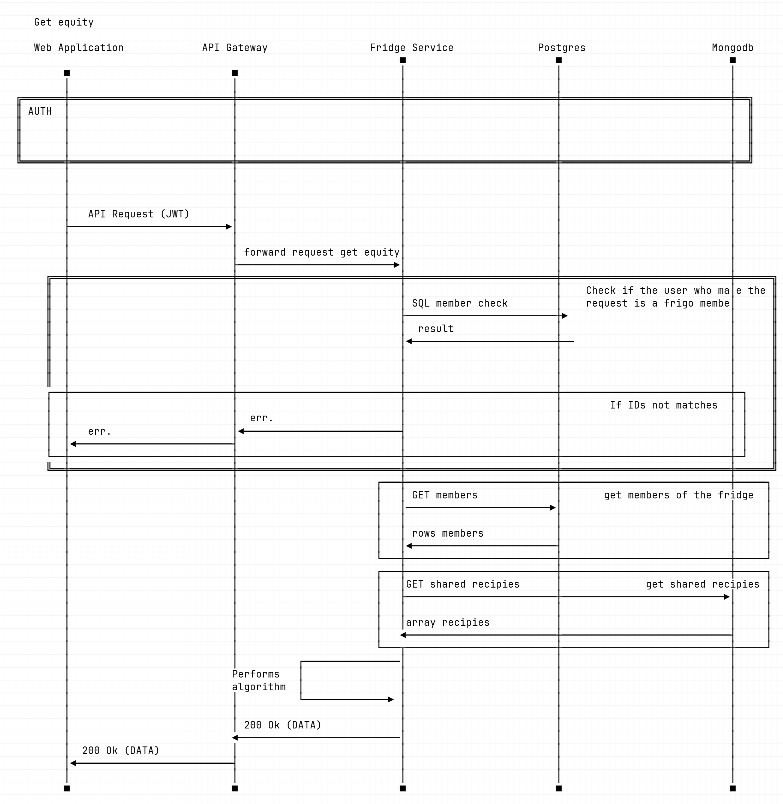
\includegraphics[width=\textwidth, height=\textheight, keepaspectratio]{get_equity.jpg}
  \caption{Sequence Diagram -- Calcolo Distribuzione Equa dei Contributi (UC10)}
  \label{fig:seq_equity}
\end{figure}

\newpage

\subsection{Rimozione Utente dal Frigorifero}

Il diagramma illustra il flusso di rimozione forzata di un membro (UC12), eseguibile esclusivamente dall'utente con ruolo \texttt{OWNER}. Il frontend invia una richiesta \texttt{DELETE /api/v1/fridges/:fridgeId/members/:userId} al Gateway, che dopo la verifica del token inietta le credenziali dell'utente richiedente negli header. Il Fridge Service verifica innanzitutto che il richiedente sia OWNER del frigorifero tramite una query su \texttt{FRIDGE\_MEMBERS}; se il controllo fallisce risponde \texttt{403 Forbidden}. Se il controllo passa, il servizio elimina il record corrispondente all'utente target in \texttt{FRIDGE\_MEMBERS} e restituisce \texttt{200 OK}. Il membro rimosso, al successivo accesso all'applicazione, non vedrà più il frigorifero nella propria Dashboard poiché la query \texttt{GET /fridges} filtra i risultati sulla base dell'appartenenza corrente.

\begin{figure}[H]
  \centering
  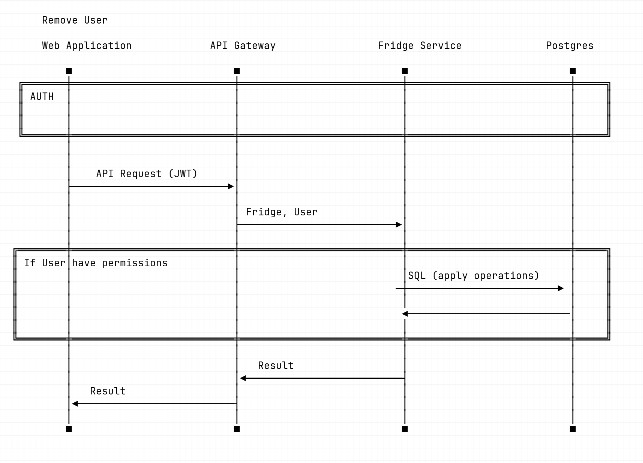
\includegraphics[width=\textwidth, height=\textheight, keepaspectratio]{remove_user.jpg}
  \caption{Sequence Diagram -- Espulsione di un Membro dal Frigorifero (UC12)}
  \label{fig:seq_remove}
\end{figure}

\newpage
\section{Testing -- Iterazione 2}

\subsection{Analisi Dinamica -- Fridge Service e Recipe Service}

Nell'Iterazione 2 la copertura dei test è stata estesa al \texttt{fridge-service} e al \texttt{recipe-service}. I test del \texttt{fridge-service} coprono i nuovi endpoint relativi alla gestione dei membri (rimozione, uscita) e al calcolo dell'equità. I test del \texttt{recipe-service} verificano il corretto inoltro della richiesta all'API OpenAI e la gestione degli errori in caso di risposta non valida.

\begin{figure}[H]
  \centering
  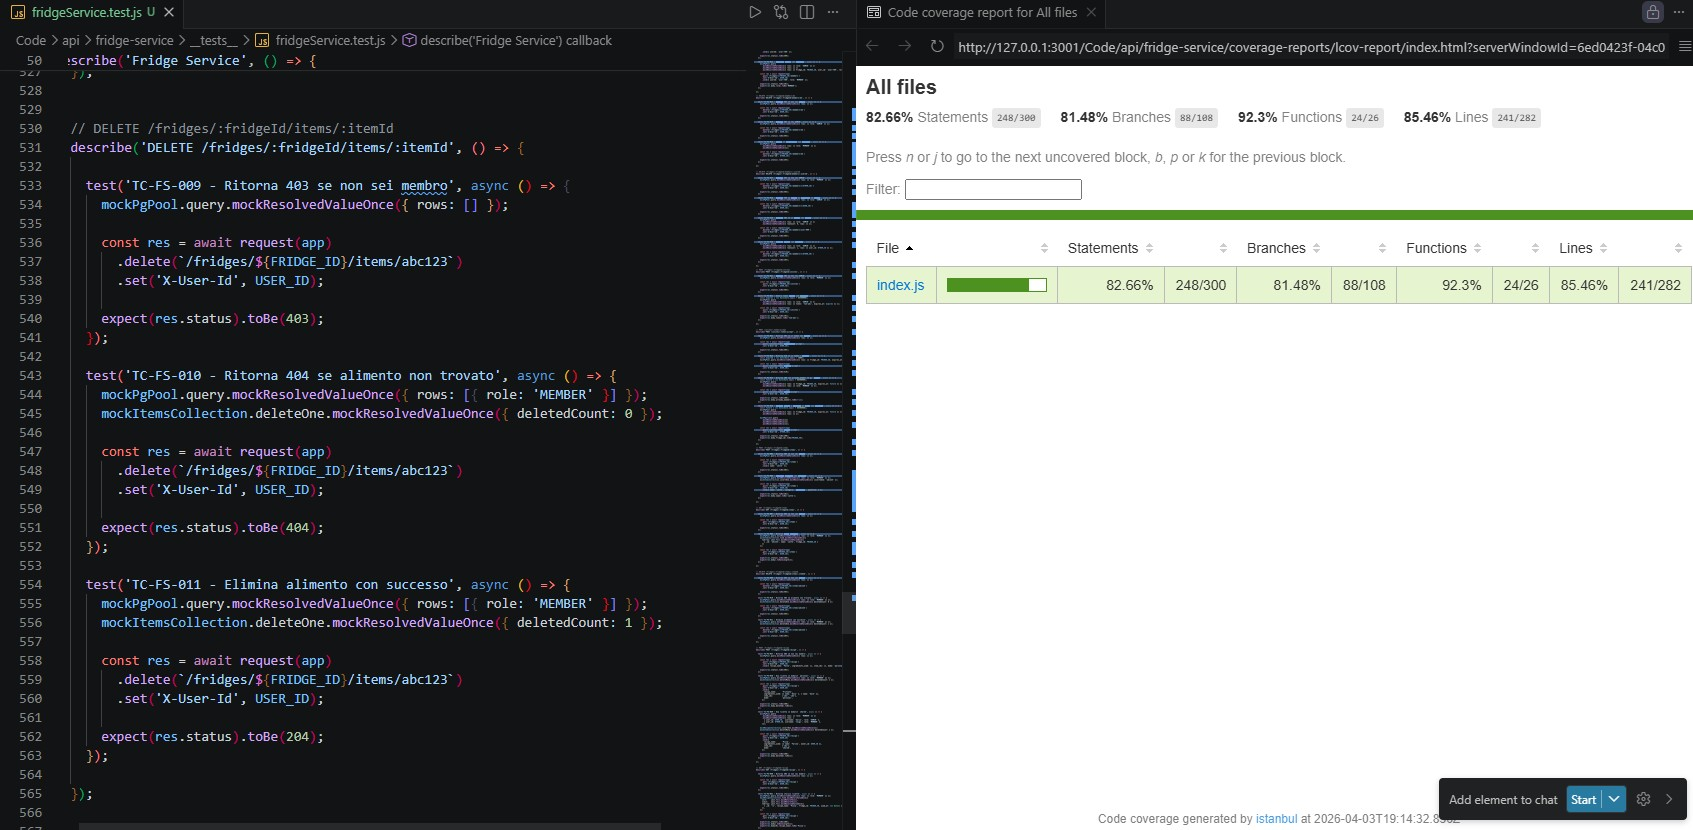
\includegraphics[width=\textwidth, height=\textheight, keepaspectratio]{Coverage-fridge.jpg}
  \caption{Report di Coverage -- Fridge Service (Iterazione 2)}
  \label{fig:cov_fridge}
\end{figure}

\begin{figure}[H]
  \centering
  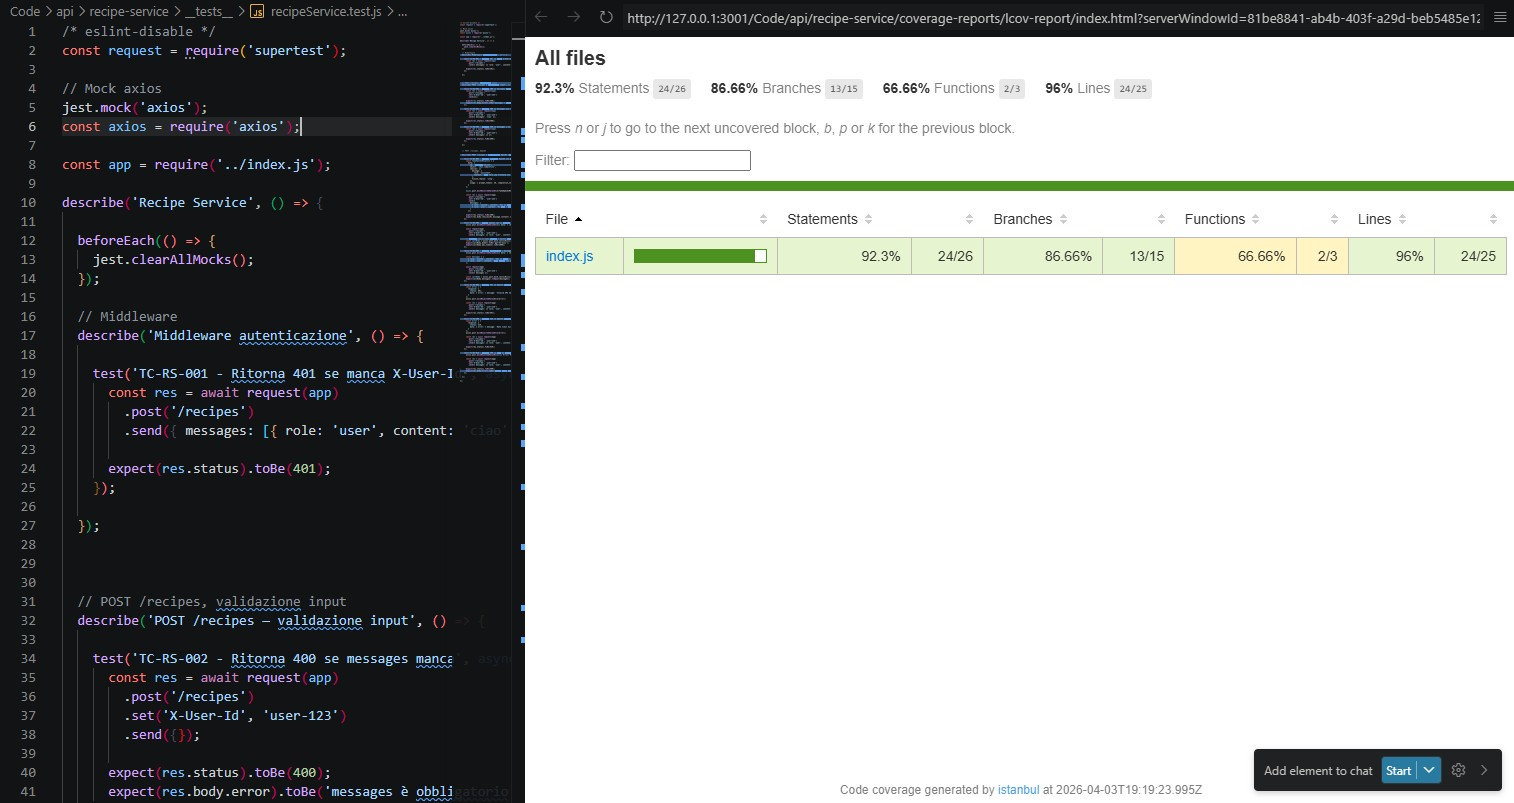
\includegraphics[width=\textwidth, height=\textheight, keepaspectratio]{Coverage-recipie.jpg}
  \caption{Report di Coverage -- Recipe Service (Iterazione 2)}
  \label{fig:cov_recipe}
\end{figure}

\section{Documentazione API -- Iterazione 2}

Le tre API introdotte in questa iterazione coprono le funzionalità di equità, generazione ricette e gestione dei membri.

\subsection{Calcolo Equità e Generazione Ricetta}

\texttt{GET /api/v1/fridges/:fridgeId/equity} non accetta parametri nel body e non modifica alcuno stato; è un endpoint di sola lettura che aggrega dati da PostgreSQL e MongoDB in tempo reale. La risposta è un oggetto JSON con chiave \texttt{userId} e valore il bilancio del contributo, espresso nell'unità monetaria stimata.

\texttt{POST /api/v1/recipes} riceve nel body un array \texttt{messages} contenente la lista degli ingredienti selezionati formattata come prompt. Il Recipe Service la inoltra direttamente all'API OpenAI e restituisce al client la risposta dell'LLM senza ulteriori elaborazioni, delegando al frontend il parsing e la visualizzazione delle ricette suggerite.

\begin{figure}[H]
  \centering
  \begin{minipage}[t]{0.48\textwidth}
    \centering
    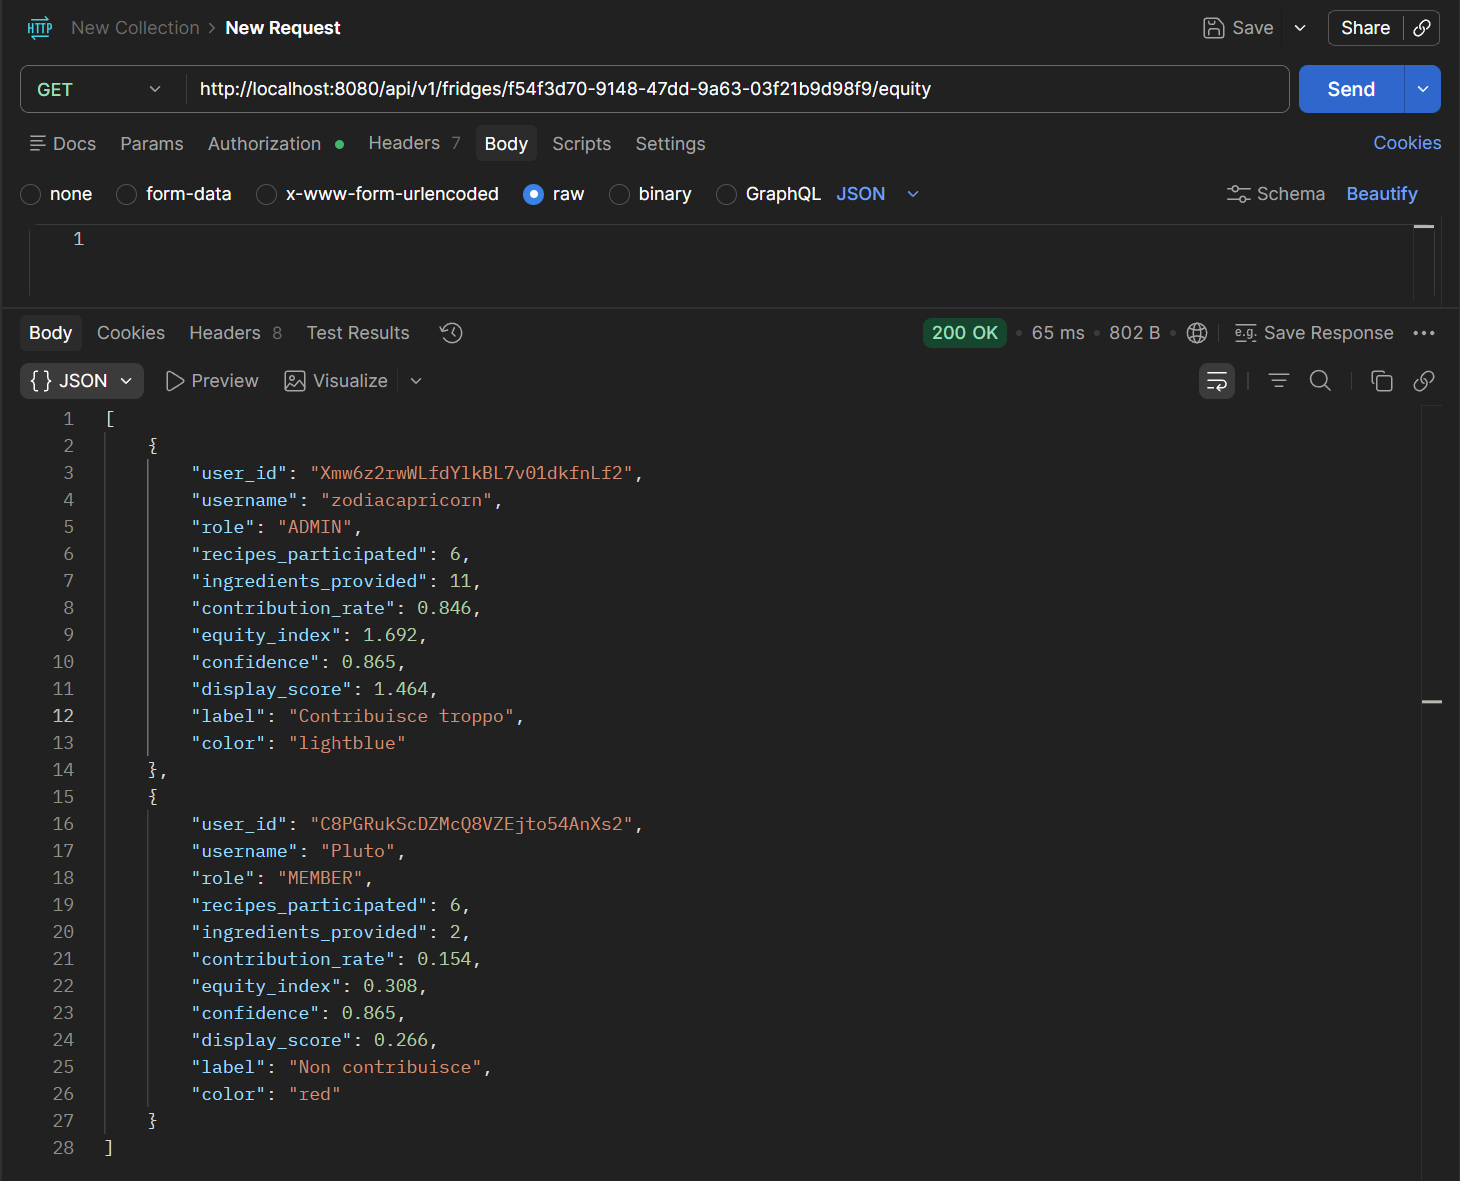
\includegraphics[width=\linewidth, height=0.28\textheight, keepaspectratio]{equity.PNG}
    \caption{GET /api/v1/fridges/:id/equity}
    \label{fig:api_equity}
  \end{minipage}
  \hfill
  \begin{minipage}[t]{0.48\textwidth}
    \centering
    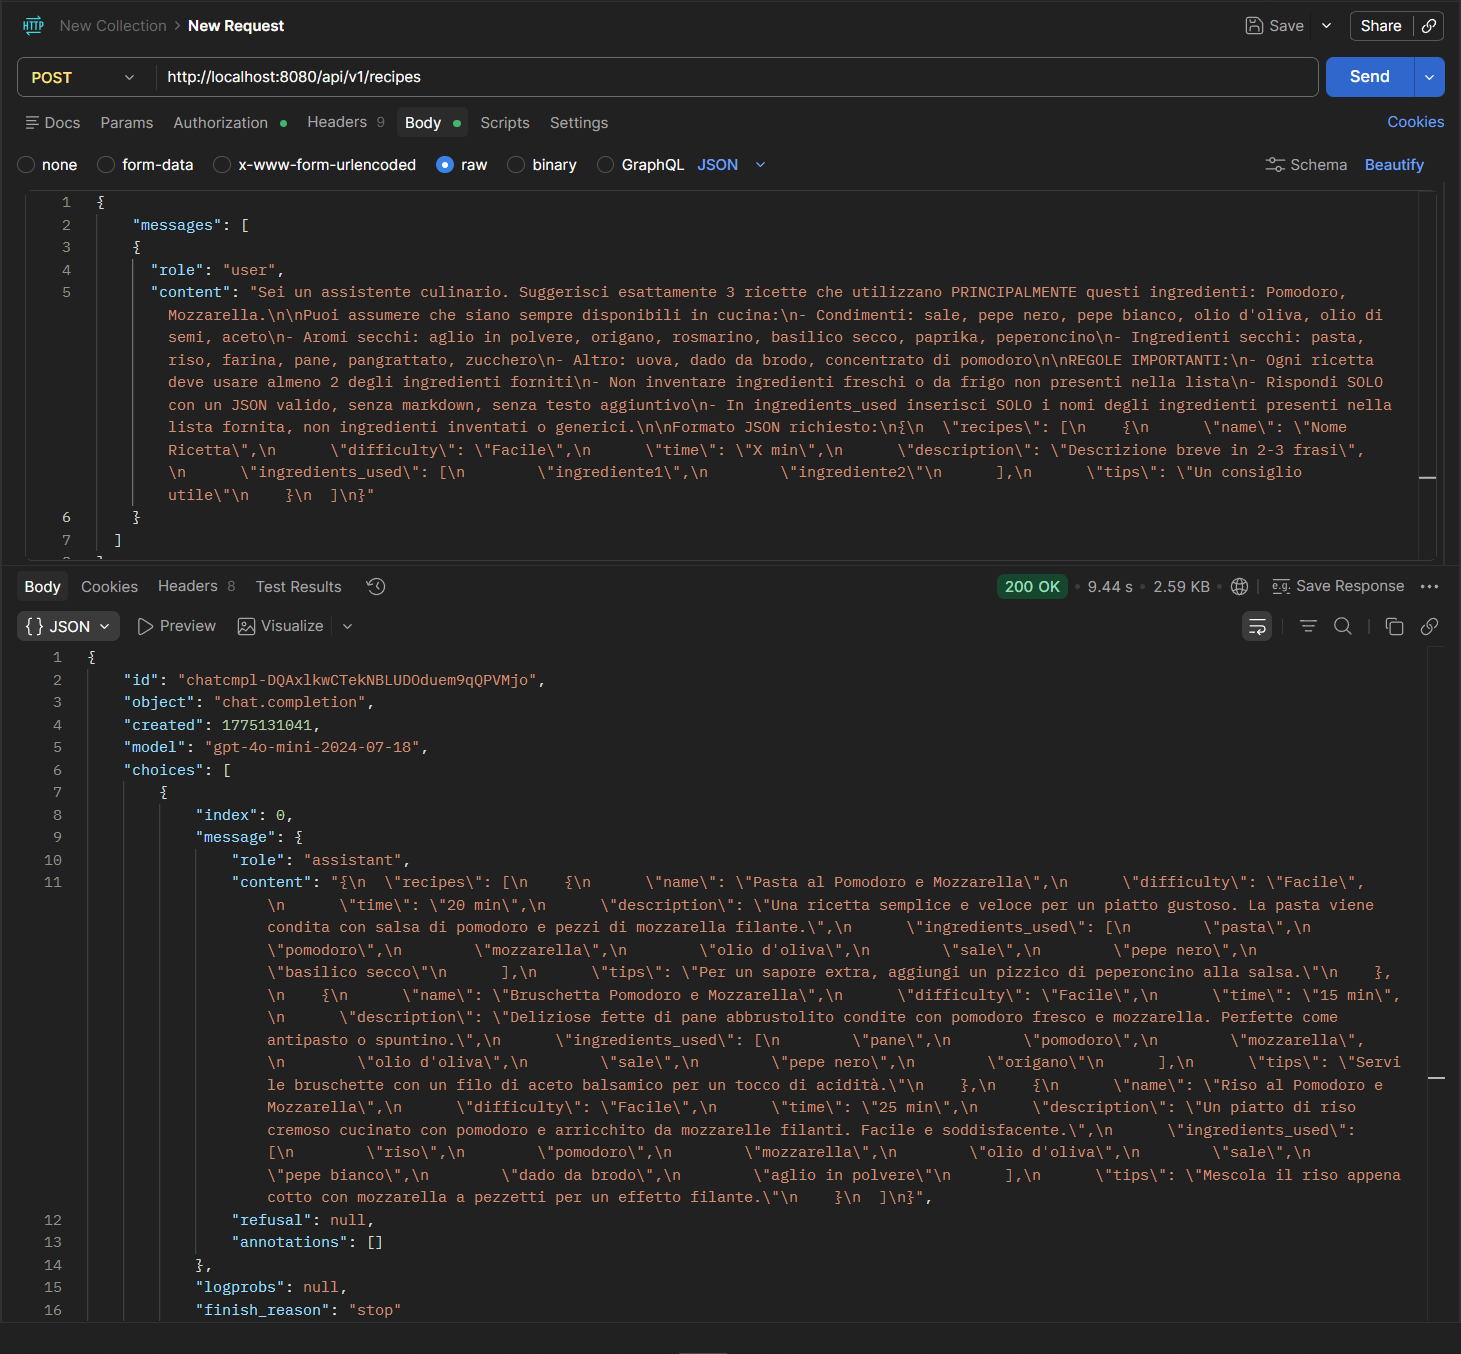
\includegraphics[width=\linewidth, height=0.28\textheight, keepaspectratio]{recipes.PNG}
    \caption{POST /api/v1/recipes}
    \label{fig:api_recipe}
  \end{minipage}
\end{figure}

\subsection{Rimozione Membro}

\texttt{DELETE /api/v1/fridges/:fridgeId/members/:userId} rimuove il membro identificato da \texttt{userId} dal frigorifero. Come illustrato nel sequence diagram corrispondente, l'operazione è riservata all'OWNER: il Fridge Service verifica il ruolo del richiedente prima di procedere e risponde \texttt{403 Forbidden} se il controllo fallisce. In caso di successo risponde \texttt{200 OK} con un messaggio di conferma; il membro rimosso perde immediatamente l'accesso all'inventario.

\begin{figure}[H]
  \centering
  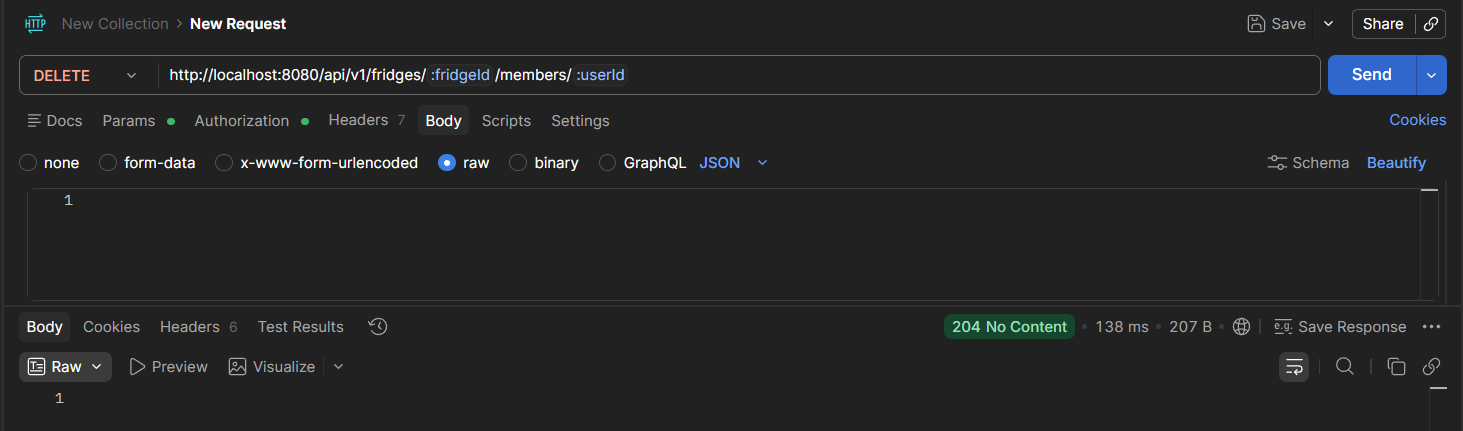
\includegraphics[width=0.75\textwidth, height=0.32\textheight, keepaspectratio]{espulsione.PNG}
  \caption{DELETE /api/v1/fridges/:id/members/:userId}
  \label{fig:api_expulsion}
\end{figure}

\newpage
\chapter{Infrastruttura CI/CD}

\section{Continuous Integration e Continuous Delivery}

All'interno dell'odierno panorama dell'ingegneria del software, l'implementazione di pratiche di automazione per il rilascio del codice risulta fondamentale per garantire scalabilità, affidabilità e rapidità d'esecuzione. In questo progetto è stata implementata una pipeline di \textbf{Continuous Integration e Continuous Delivery (CI/CD)} basata su \textbf{GitHub Actions}, specificamente ingegnerizzata per gestire un'architettura a microservizi ospitata all'interno di un monorepo. L'infrastruttura è progettata per automatizzare rigorosamente i processi di validazione, compilazione e pacchettizzazione del software, azzerando l'intervento manuale e riducendo significativamente il margine di errore sistemico.

\section{Triggers e Filtri di Percorso}

Il processo di automazione è configurato per avviarsi in modo continuo a ogni modifica del codice sul ramo principale (\texttt{main}), fungendo da barriera di transizione tra lo sviluppo e l'ambiente di produzione. È altresì prevista l'esecuzione manuale (\texttt{workflow\_dispatch}) per garantire flessibilità operativa in scenari di ripristino o rilasci forzati.

Operando in un contesto monorepo, la pipeline implementa \textbf{filtri di percorso} per identificare in modo granulare quali specifici microservizi (es.\ \texttt{gateway}, \texttt{fridge-service}, \texttt{user-service}) abbiano subito mutazioni. Questo approccio selettivo garantisce un'ottimizzazione delle risorse computazionali, istruendo il sistema a eseguire i successivi processi di validazione e compilazione esclusivamente per i moduli effettivamente modificati, riducendo drasticamente i tempi di esecuzione complessivi (\textit{time-to-market}).

La figura~\ref{fig:cicd2} mostra la struttura del grafo di esecuzione (\textit{workflow DAG}) nello stato \textit{Queued}, evidenziando come il job \texttt{detect-changes} si ramifichi in parallelo verso i job di test e build per ogni servizio modificato. La figura~\ref{fig:cicd4} mostra lo stesso workflow al termine dell'esecuzione con stato \textit{Success}, confermando il completamento di tutte le fasi.

\begin{figure}[H]
  \centering
  \begin{minipage}[t]{\textwidth}
    \centering
    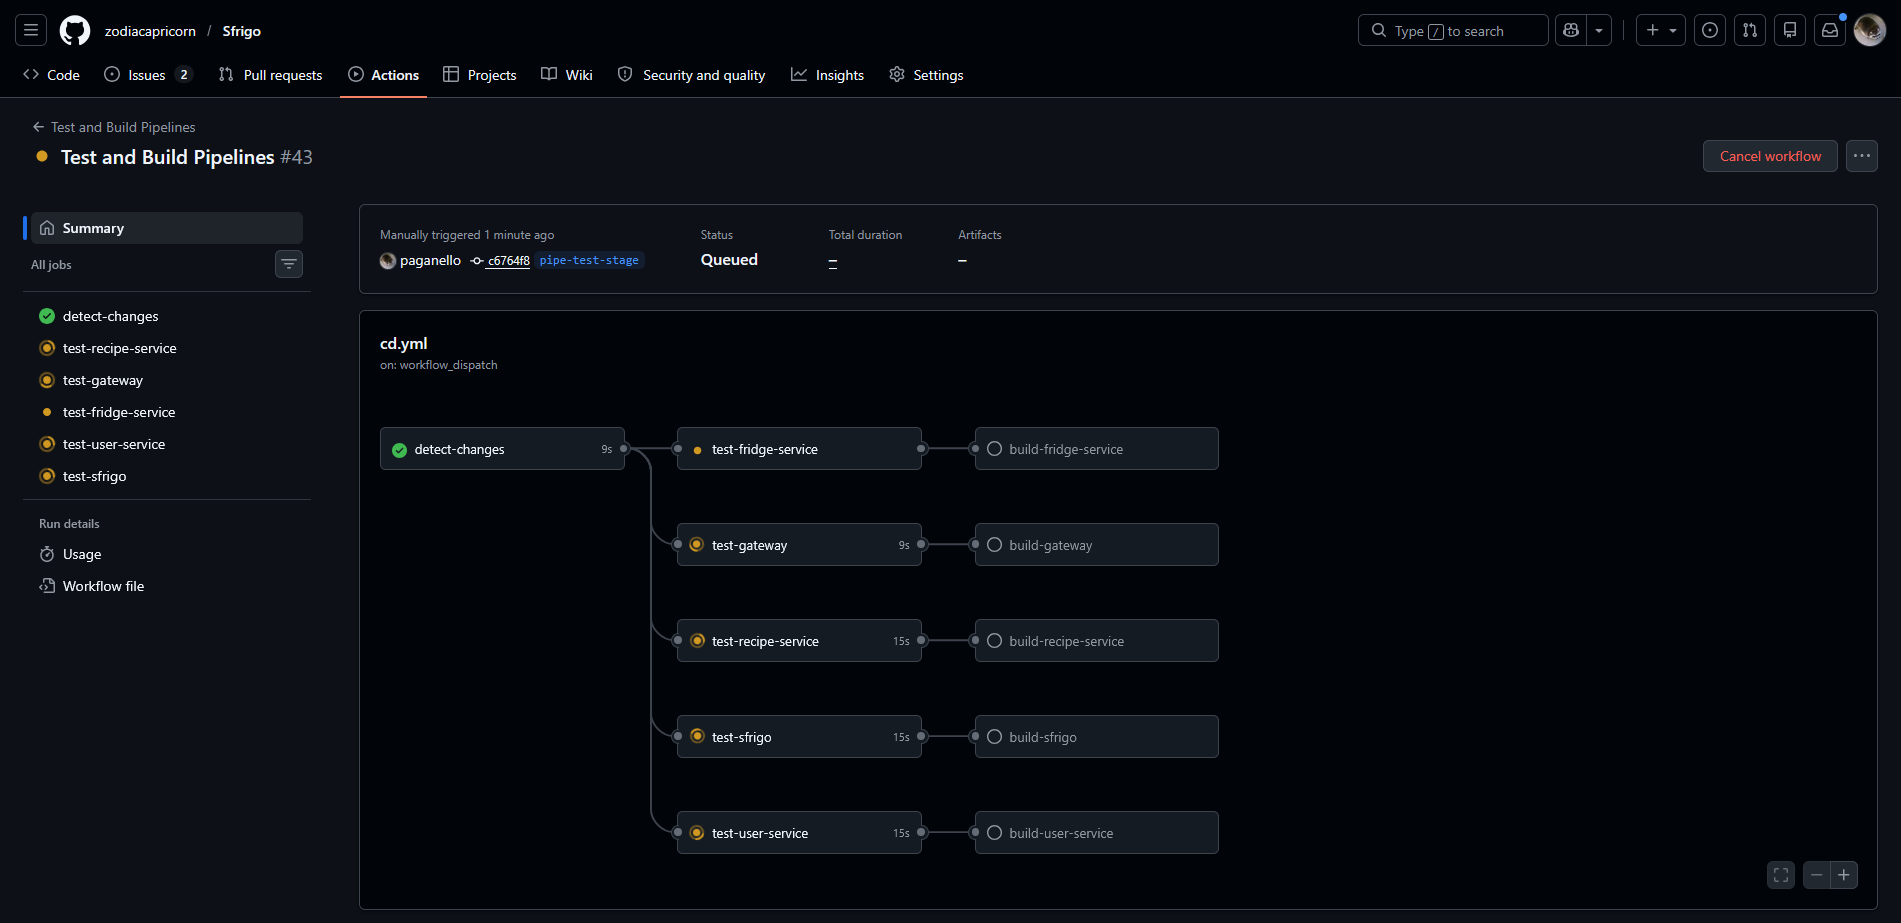
\includegraphics[width=\linewidth, height=0.28\textheight, keepaspectratio]{2.PNG}
    \caption{Workflow DAG -- stato \textit{Queued}}
    \label{fig:cicd2}
  \end{minipage}
  \hfill
  \begin{minipage}[t]{\textwidth}
    \centering
    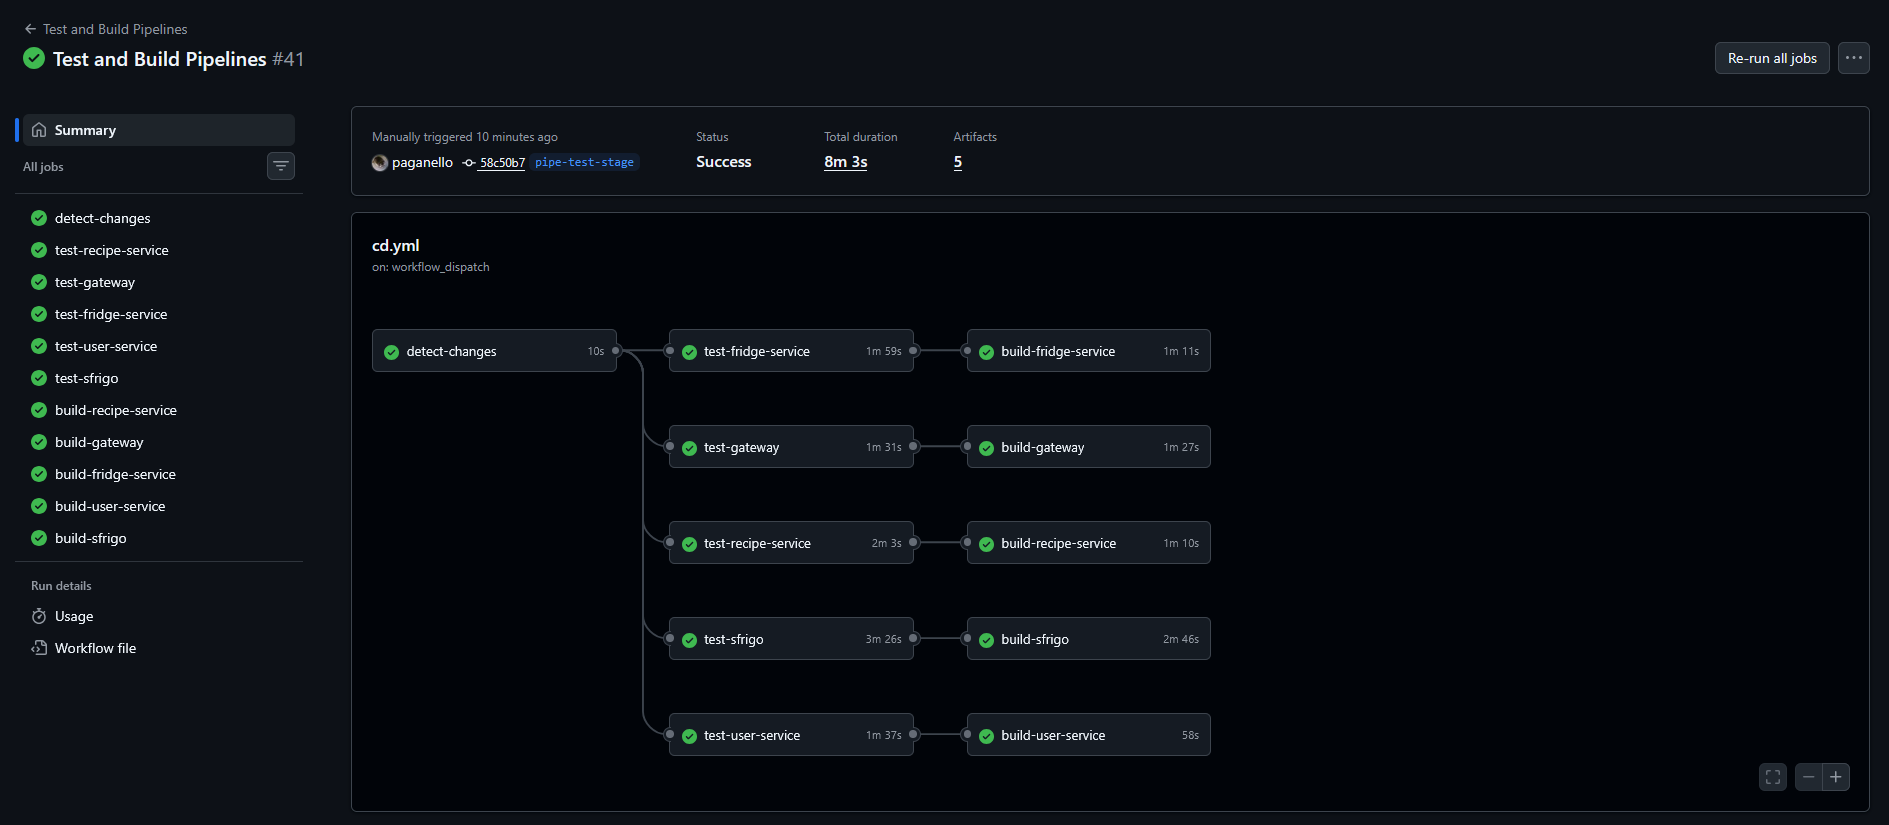
\includegraphics[width=\linewidth, height=0.28\textheight, keepaspectratio]{4.PNG}
    \caption{Workflow DAG -- stato \textit{Success}}
    \label{fig:cicd4}
  \end{minipage}
\end{figure}

\section{Flusso della Pipeline}

Per ogni modulo, il flusso di lavoro alloca dinamicamente \textbf{ambienti di esecuzione isolati} in cui avvia le relative fasi di testing: dopo il setup delle dipendenze, il codice subisce:

\begin{itemize}
  \item un'analisi architetturale, mirata a prevenire dipendenze circolari;
  \item controlli di formattazione (\textit{linting});
  \item test unitari.
\end{itemize}

Queste fasi fungono da barriera deterministica contro la propagazione di eventuali regressioni. Esclusivamente a fronte di una validazione superata con successo, la pipeline innesca le fasi di \textit{build} e \textit{push}: previa autenticazione al Docker registry di destinazione tramite credenziali (passate via \texttt{Secrets}), il codice sorgente viene compilato in \textbf{immagini Docker}, garantendo la totale standardizzazione e idempotenza del software in ambiente produttivo.

Infine, l'artefatto viene inviato al registry e contrassegnato da una \textbf{duplice etichettatura}:
\begin{itemize}
  \item il tag \texttt{latest}, per la versione corrente;
  \item l'hash univoco del commit, per la referenza esatta.
\end{itemize}

Questa pratica è necessaria per assicurare la tracciabilità assoluta del ciclo di vita applicativo e garantire operazioni di \textit{rollback}.

La figura~\ref{fig:cicd3} riporta il log di esecuzione del job \texttt{test-fridge-service}, mostrando i test Jest con i relativi casi di test superati. La figura~\ref{fig:cicd5} mostra la pagina dei \textit{Repository Secrets} di GitHub, dove sono configurate le credenziali del Registry Docker e le variabili d'ambiente di Firebase necessarie al build del frontend.

\begin{figure}[H]
  \centering
  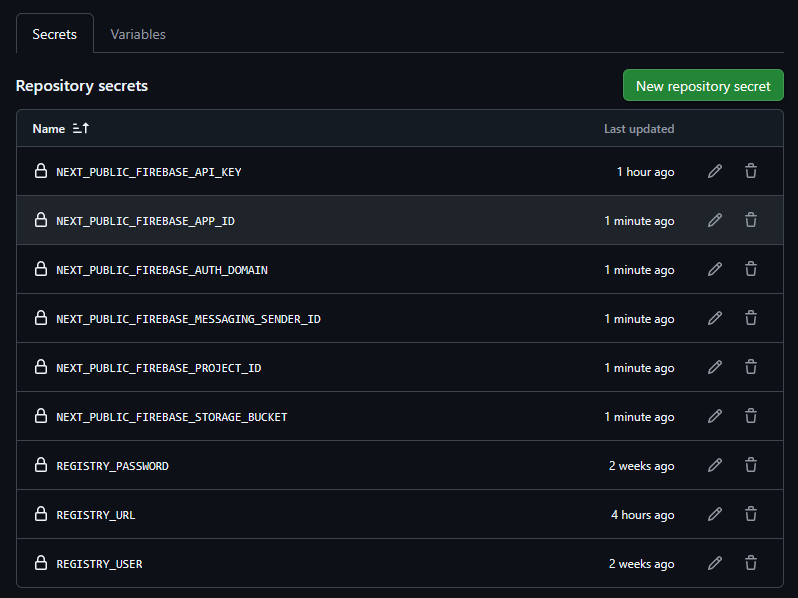
\includegraphics[width=\textwidth]{5.PNG}
  \caption{Repository Secrets -- credenziali CI/CD}
  \label{fig:cicd5}
\end{figure}

\begin{figure}[H]
  \centering
  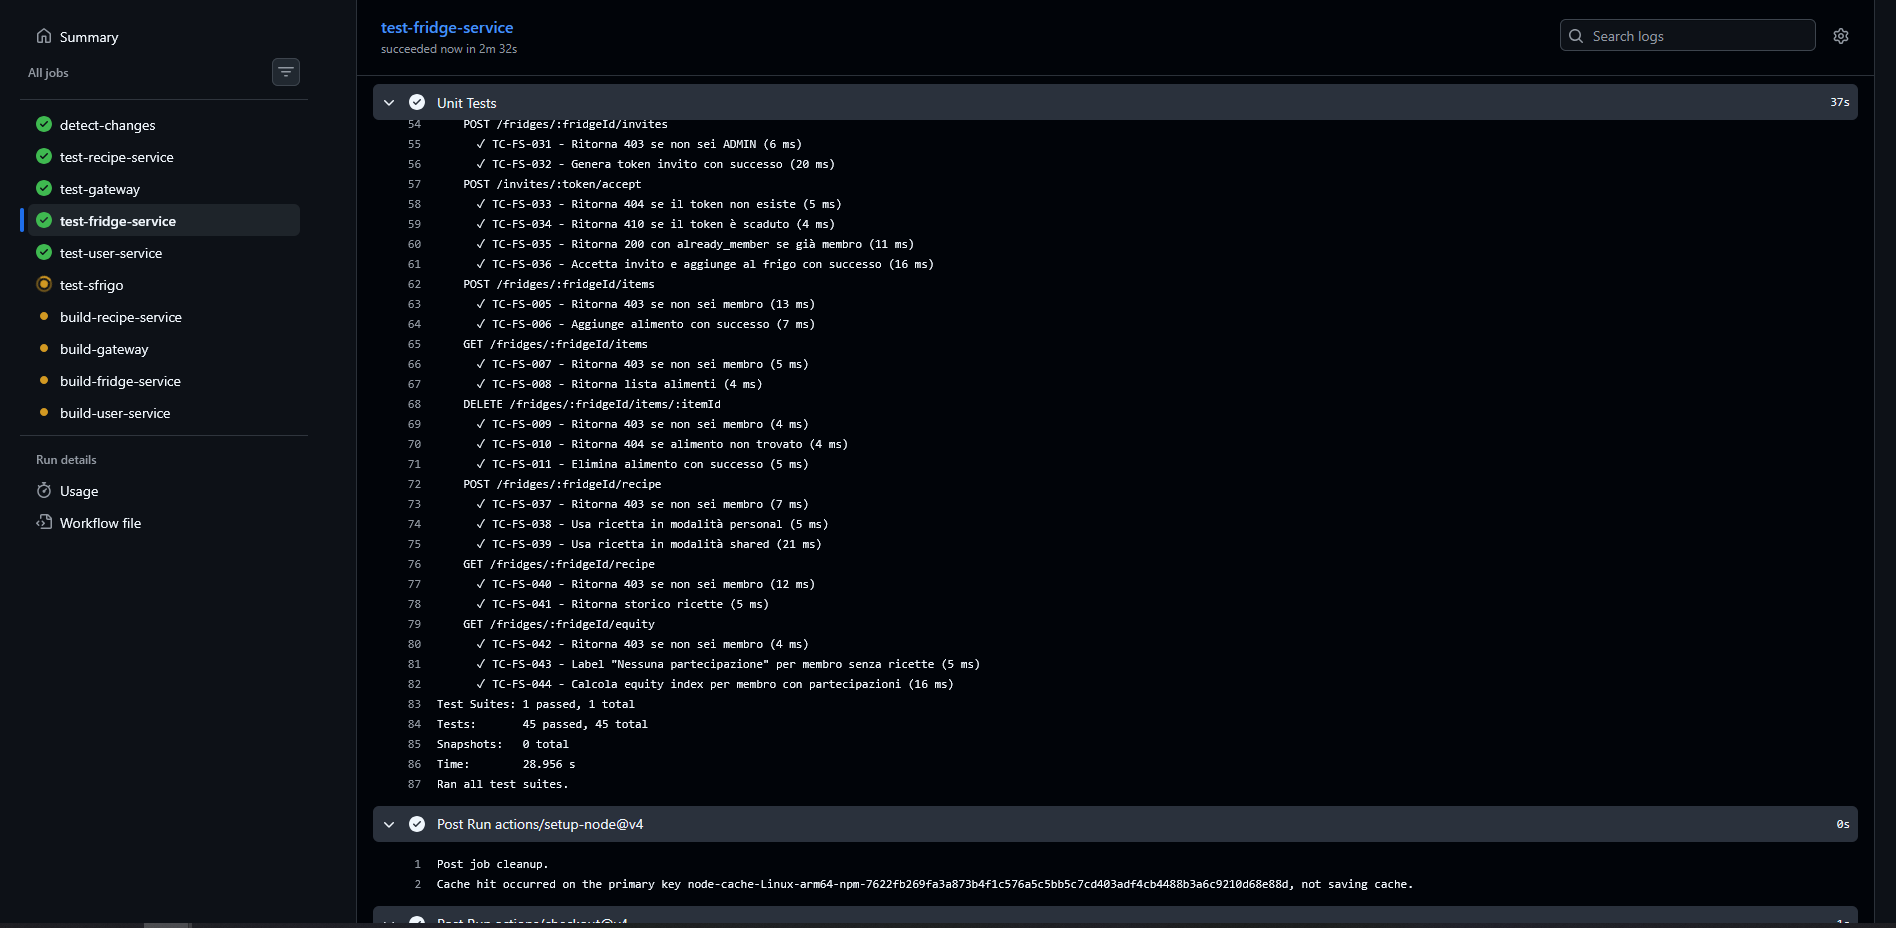
\includegraphics[width=0.95\textwidth]{3.PNG}
  \caption{Log del job \texttt{test-fridge-service}}
  \label{fig:cicd3}
\end{figure}

\section{Architettura di Esecuzione}

L'infrastruttura computazionale sottostante all'esecuzione delle pipeline CI/CD si fonda su un \textbf{cluster Kubernetes} proprietario, implementato e configurato su istanze cloud con architettura ARM fornite da \textbf{Oracle Cloud Infrastructure (OCI)}. L'orchestrazione e l'allocazione dinamica dei flussi di lavoro GitHub Actions sono demandate a un \textbf{Action Runner Controller (ARC)}, operante in ascolto (\textit{listener}) all'interno del cluster stesso e direttamente interfacciato con il registro delle pipeline.

\begin{figure}[H]
  \centering
  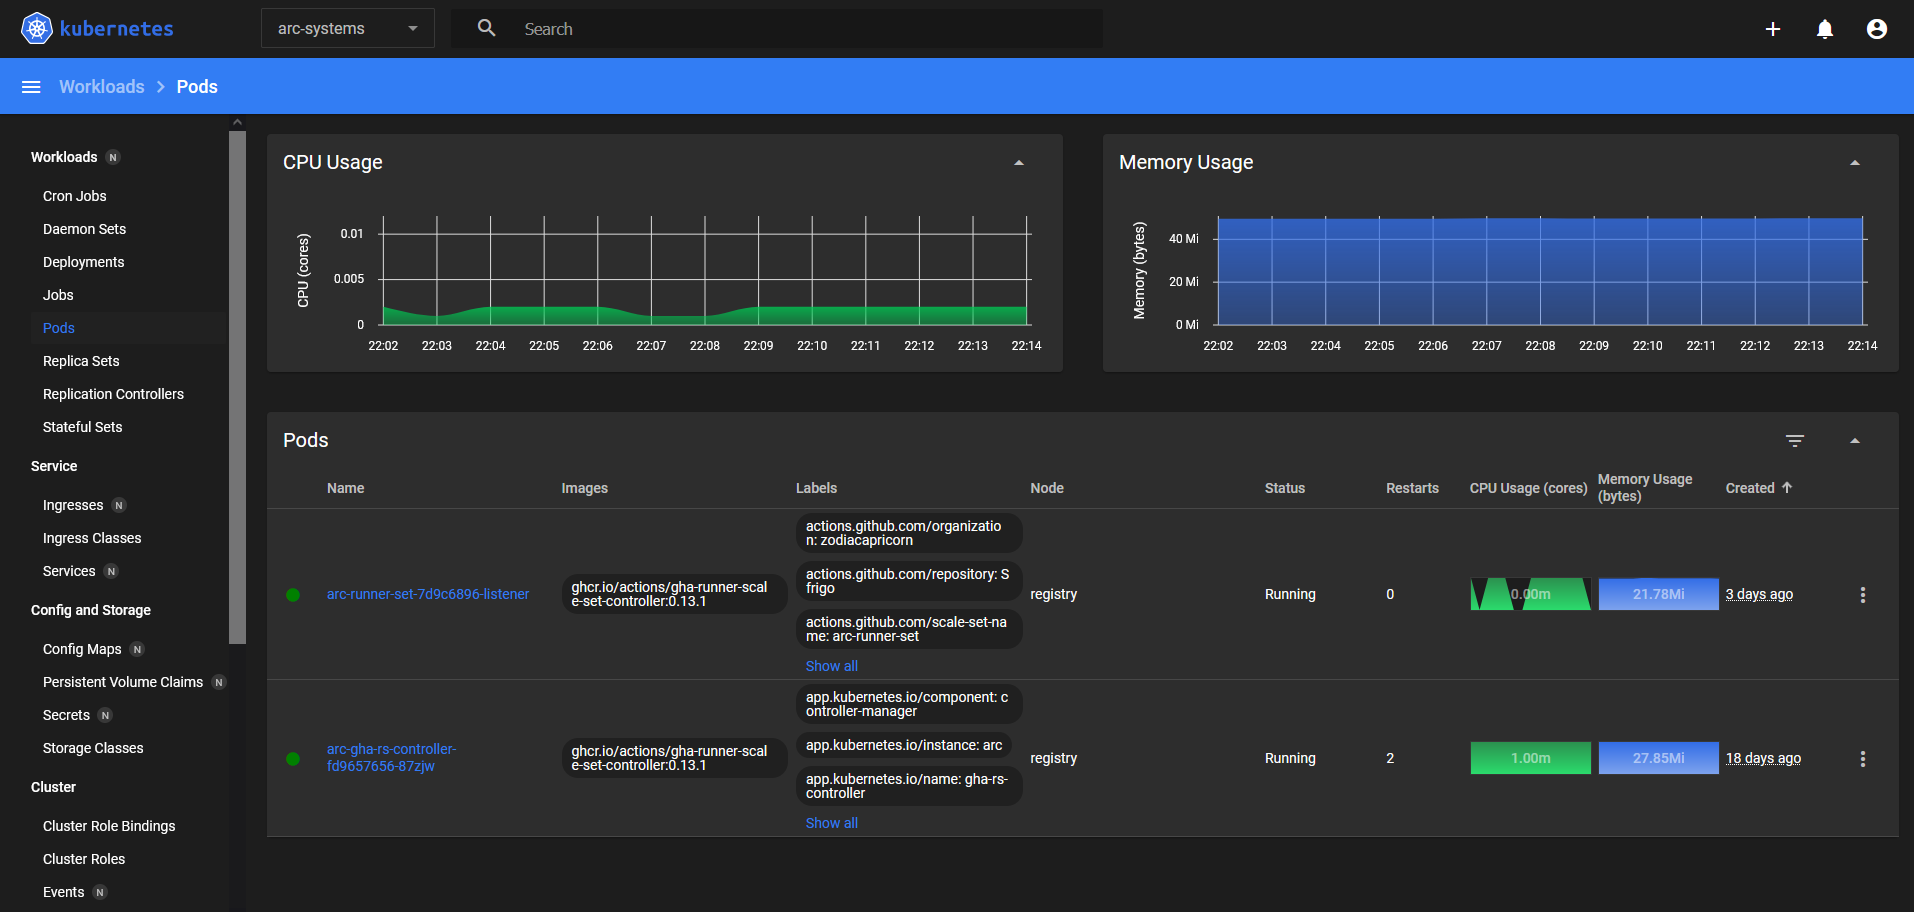
\includegraphics[width=\textwidth]{1.PNG}
  \caption{Kubernetes -- pod con image taggate dopo il deploy automatico}
  \label{fig:cicd1}
\end{figure}

\section{Architettura di Deployment e Topologia dei Servizi}

L'infrastruttura di deployment, ospitata sul cluster Kubernetes precedentemente delineato, si articola in una \textbf{topologia a microservizi} orchestrata per garantire un'elevata coesione interna e una netta separazione delle responsabilità (\textit{separation of concerns}). Come si evince dall'analisi dei carichi di lavoro (\textit{workloads}), l'intero ecosistema applicativo è logicamente segregato all'interno di un \textbf{namespace dedicato} e si compone di molteplici livelli funzionali.

Il livello di presentazione è gestito da un deployment dedicato al frontend (\textit{frontend-deployment}), affiancato da un \textbf{API Gateway} (\texttt{gateway}) che funge da mediatore per le logiche di backend. I microservizi preposti alla business logic specifica (identificati dalle immagini \texttt{fridge-service}, \texttt{recipe-service} e \texttt{user-service}) risultano incapsulati all'interno di un aggregato di elaborazione unificato (\texttt{api-deployment}), ottimizzando l'allocazione delle risorse interne.

A supporto di questi moduli operativi, lo strato di persistenza dei dati adotta un \textbf{approccio poliglotta}, impiegando deployment indipendenti per sistemi di gestione di database sia relazionali (\textbf{PostgreSQL}) sia orientati ai documenti (\textbf{MongoDB}), al fine di assecondare le eterogenee necessità di modellazione dei dati dei singoli servizi. È rilevante notare come il provisioning di tutte le componenti applicative (ad eccezione dei database standard) avvenga tramite il \textit{pull} dinamico delle immagini dal registro locale del cluster, chiudendo di fatto il ciclo di Continuous Delivery. Infine, l'esposizione dell'intero applicativo verso la rete esterna è delegata e centralizzata tramite una risorsa \textbf{Ingress}. Questo strato architetturale agisce come punto di ingresso unificato e \textit{reverse proxy}, occupandosi della risoluzione dei nomi a dominio e del routing del traffico HTTP/HTTPS dall'esterno verso i corrispondenti servizi interni al cluster.

\begin{figure}[H]
  \centering
  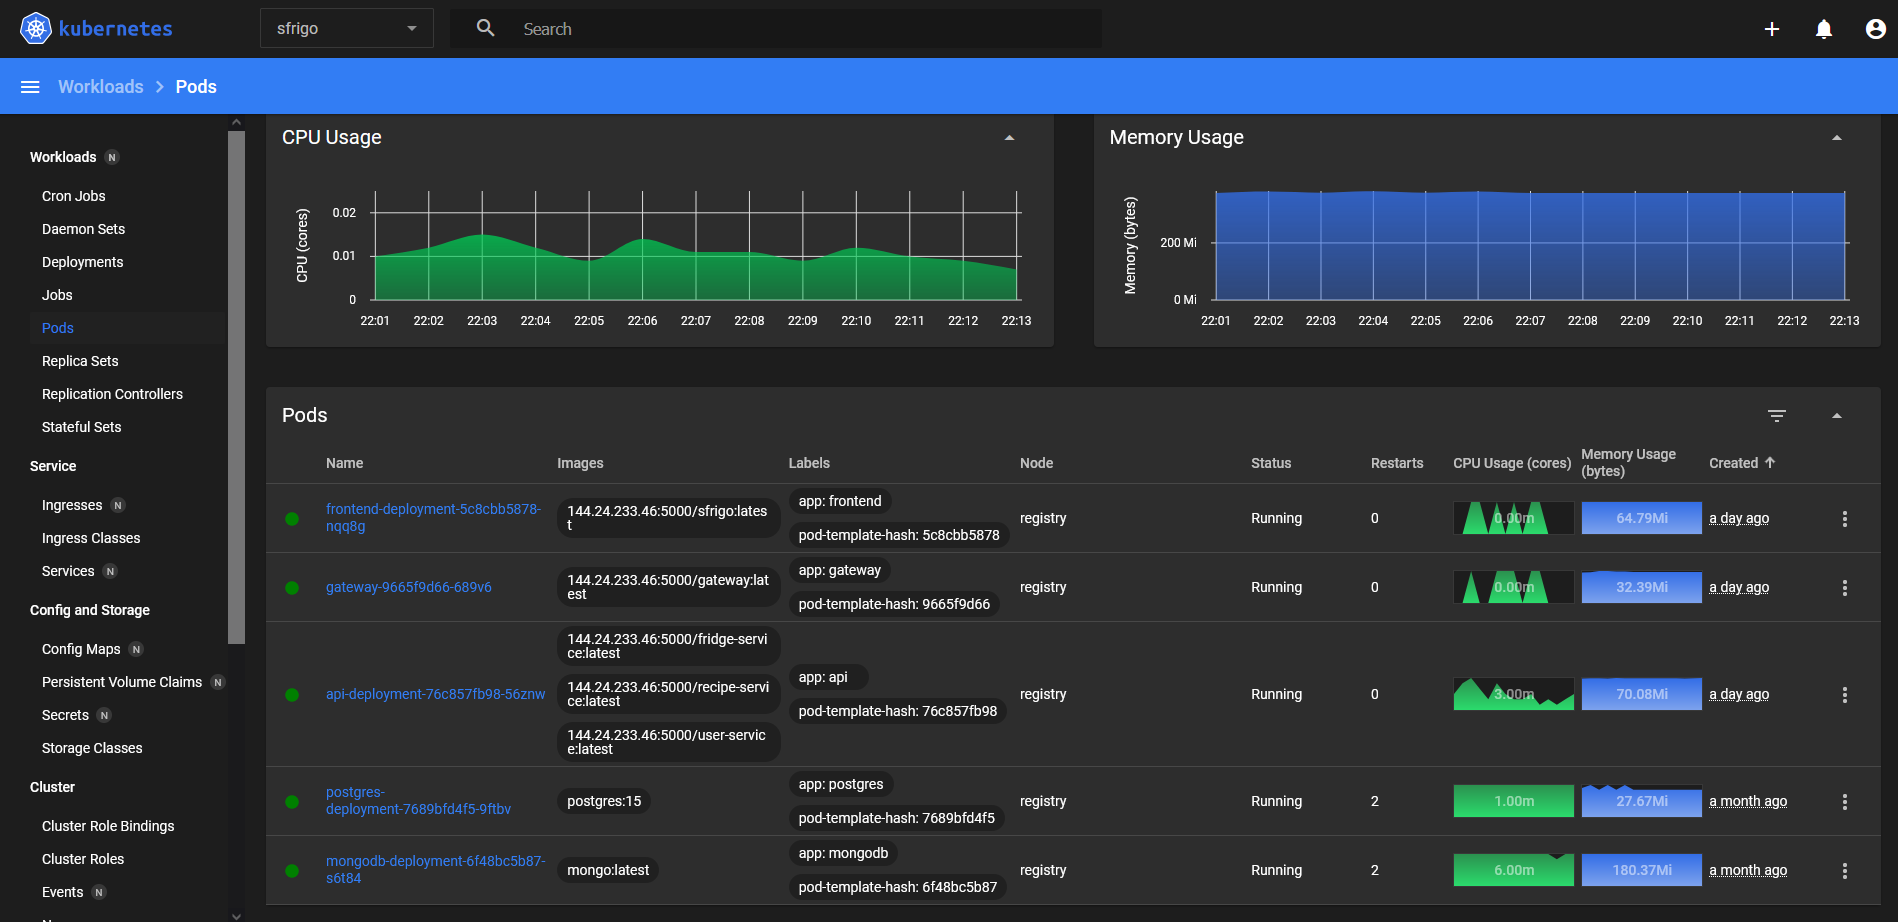
\includegraphics[width=0.80\textwidth]{0.PNG}
  \caption{Kubernetes -- namespace \texttt{sfrigo} con pod in esecuzione e metriche CPU/Memory}
  \label{fig:cicd0}
\end{figure}

\section{Implicazioni Strategiche e Aziendali}

L'adozione di questo paradigma metodologico risponde in modo esaustivo alle esigenze aziendali moderne. Strategicamente, la pipeline converte il consolidamento del codice in un rilascio tangibile e sicuro, spostando il controllo di qualità a monte del processo (\textit{shift-left testing}). Questo isola le dipendenze dei vari microservizi, permettendo ai team di sviluppo di rilasciare aggiornamenti in totale autonomia e parallelismo, massimizzando l'efficienza delle risorse, mitigando il rischio di deployment e garantendo un flusso continuo e ininterrotto di valore verso l'utente finale.

\begin{figure}[H]
  \centering
  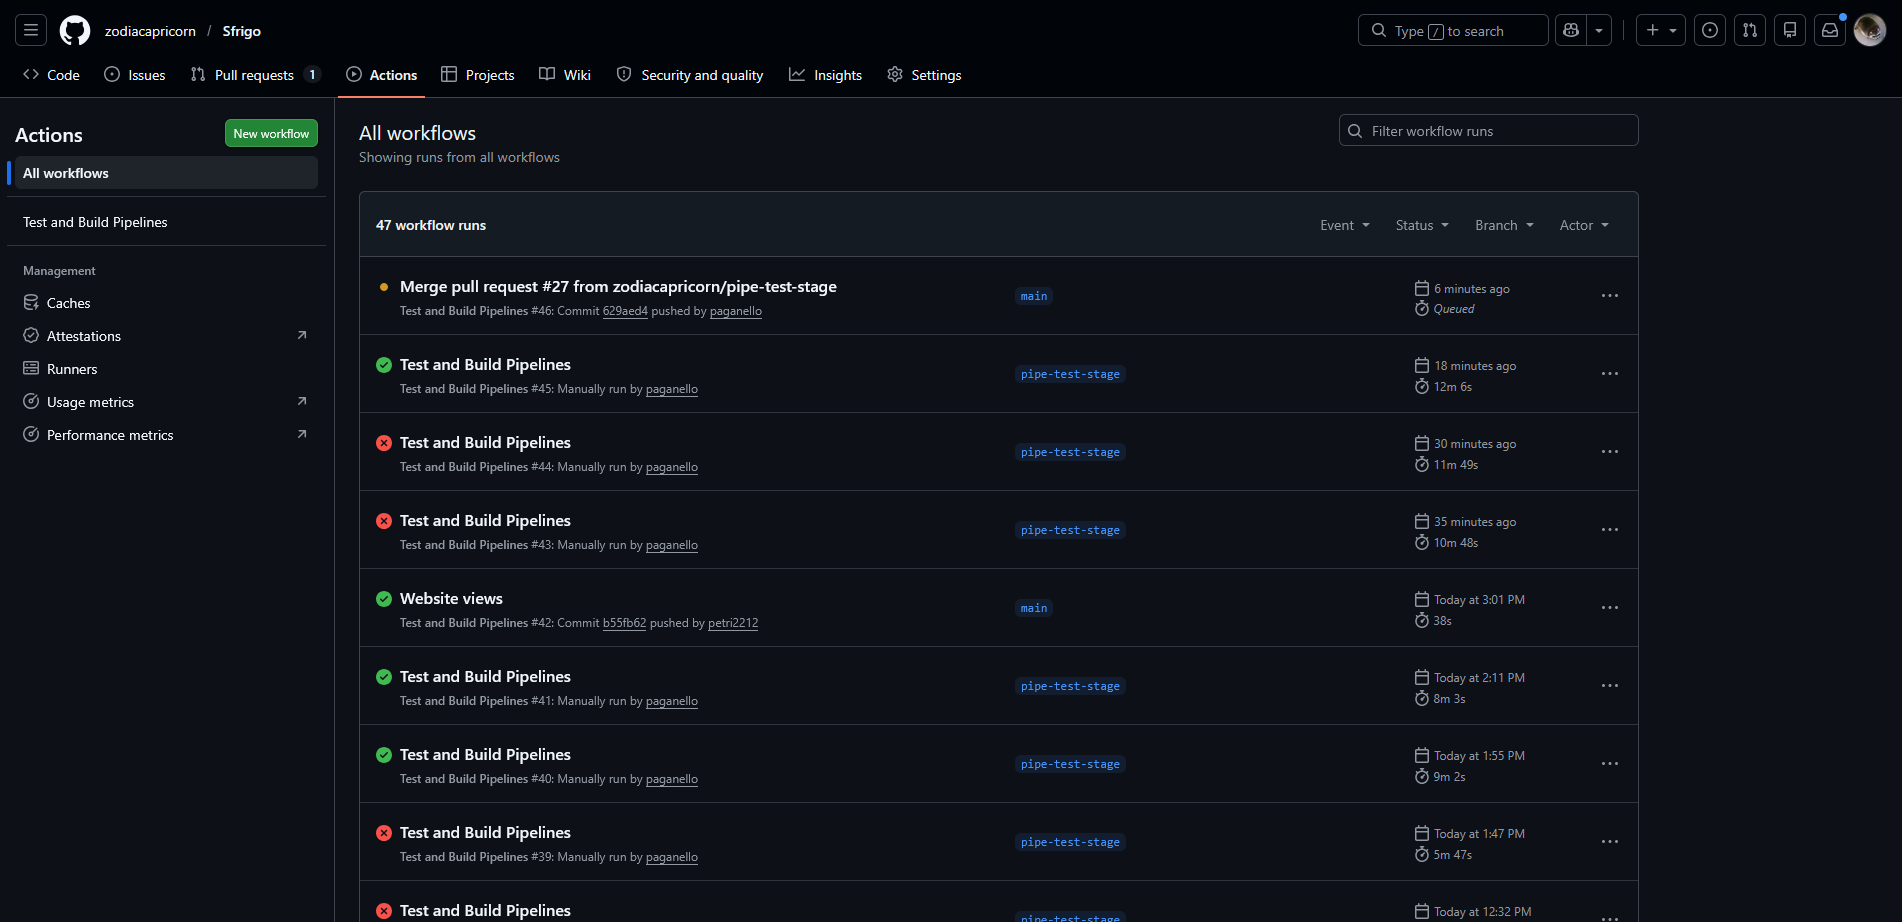
\includegraphics[width=\textwidth]{6.PNG}
  \caption{GitHub Actions -- storico dei workflow run con indicazione degli stati}
  \label{fig:cicd6}
\end{figure}

\newpage
\chapter{Viste Frontend}

\begin{figure}[H]
  \centering
  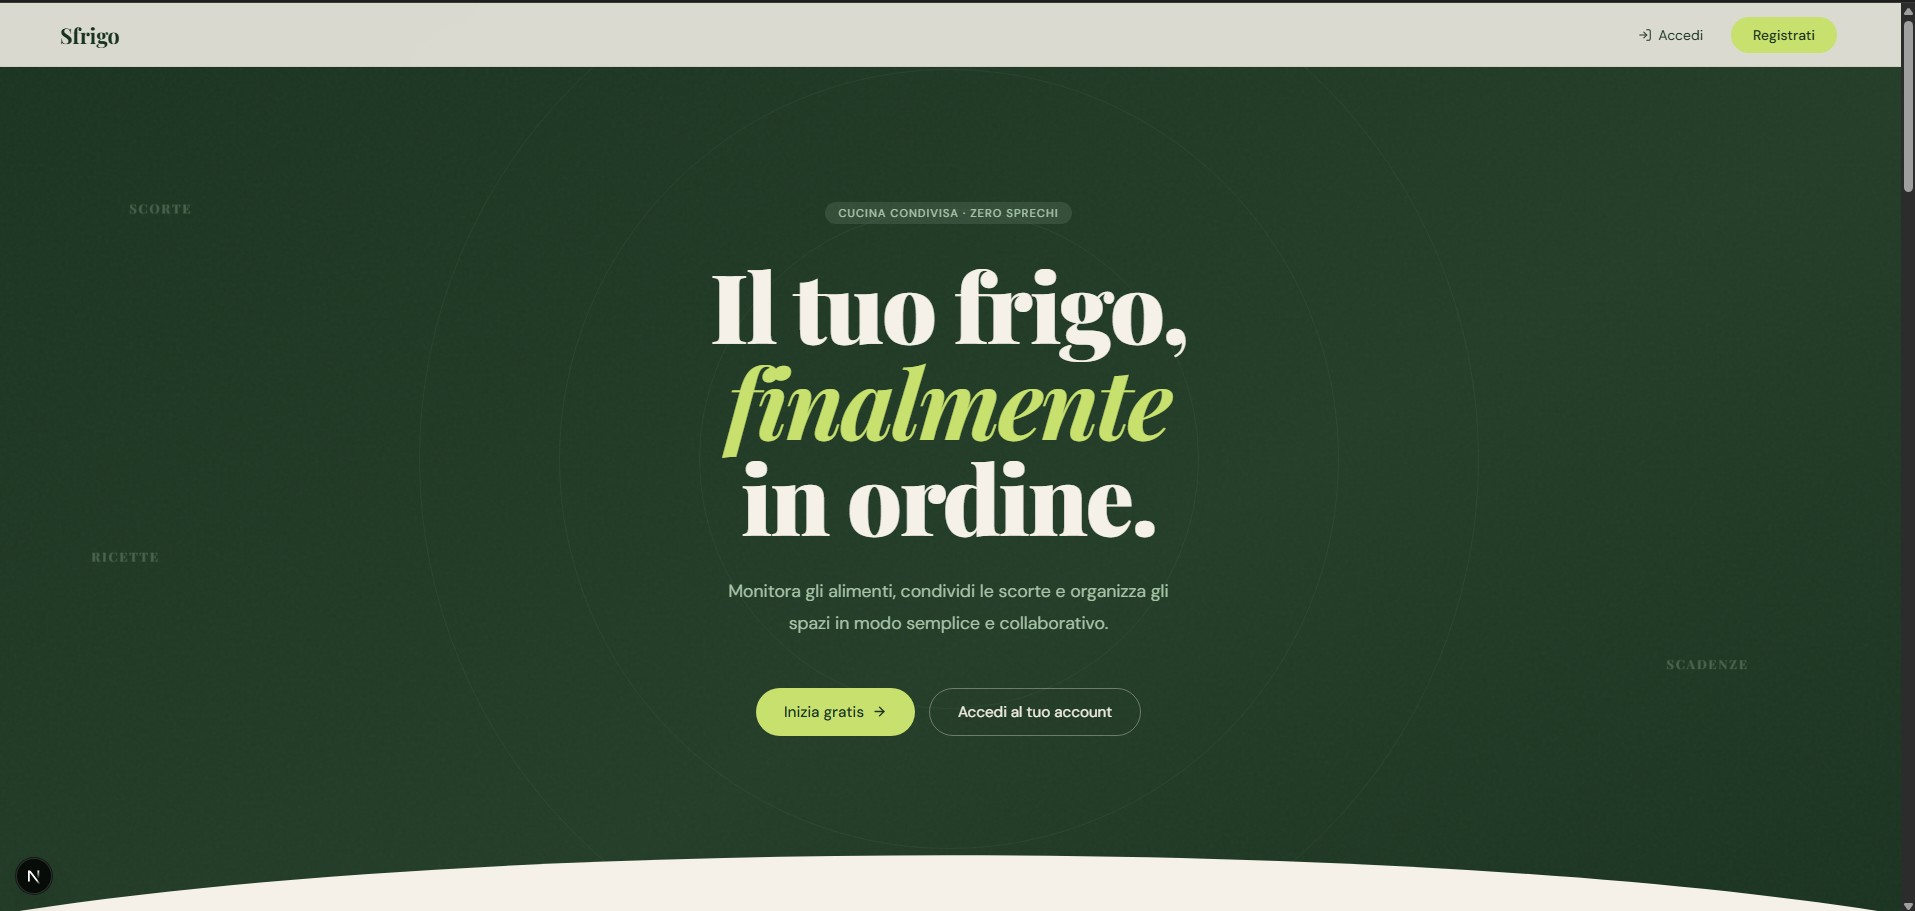
\includegraphics[width=\textwidth]{./img/home.jpg}
  \caption{Homepage del sito web}
  \label{fig:home}
\end{figure}

\begin{figure}[H]
  \centering
  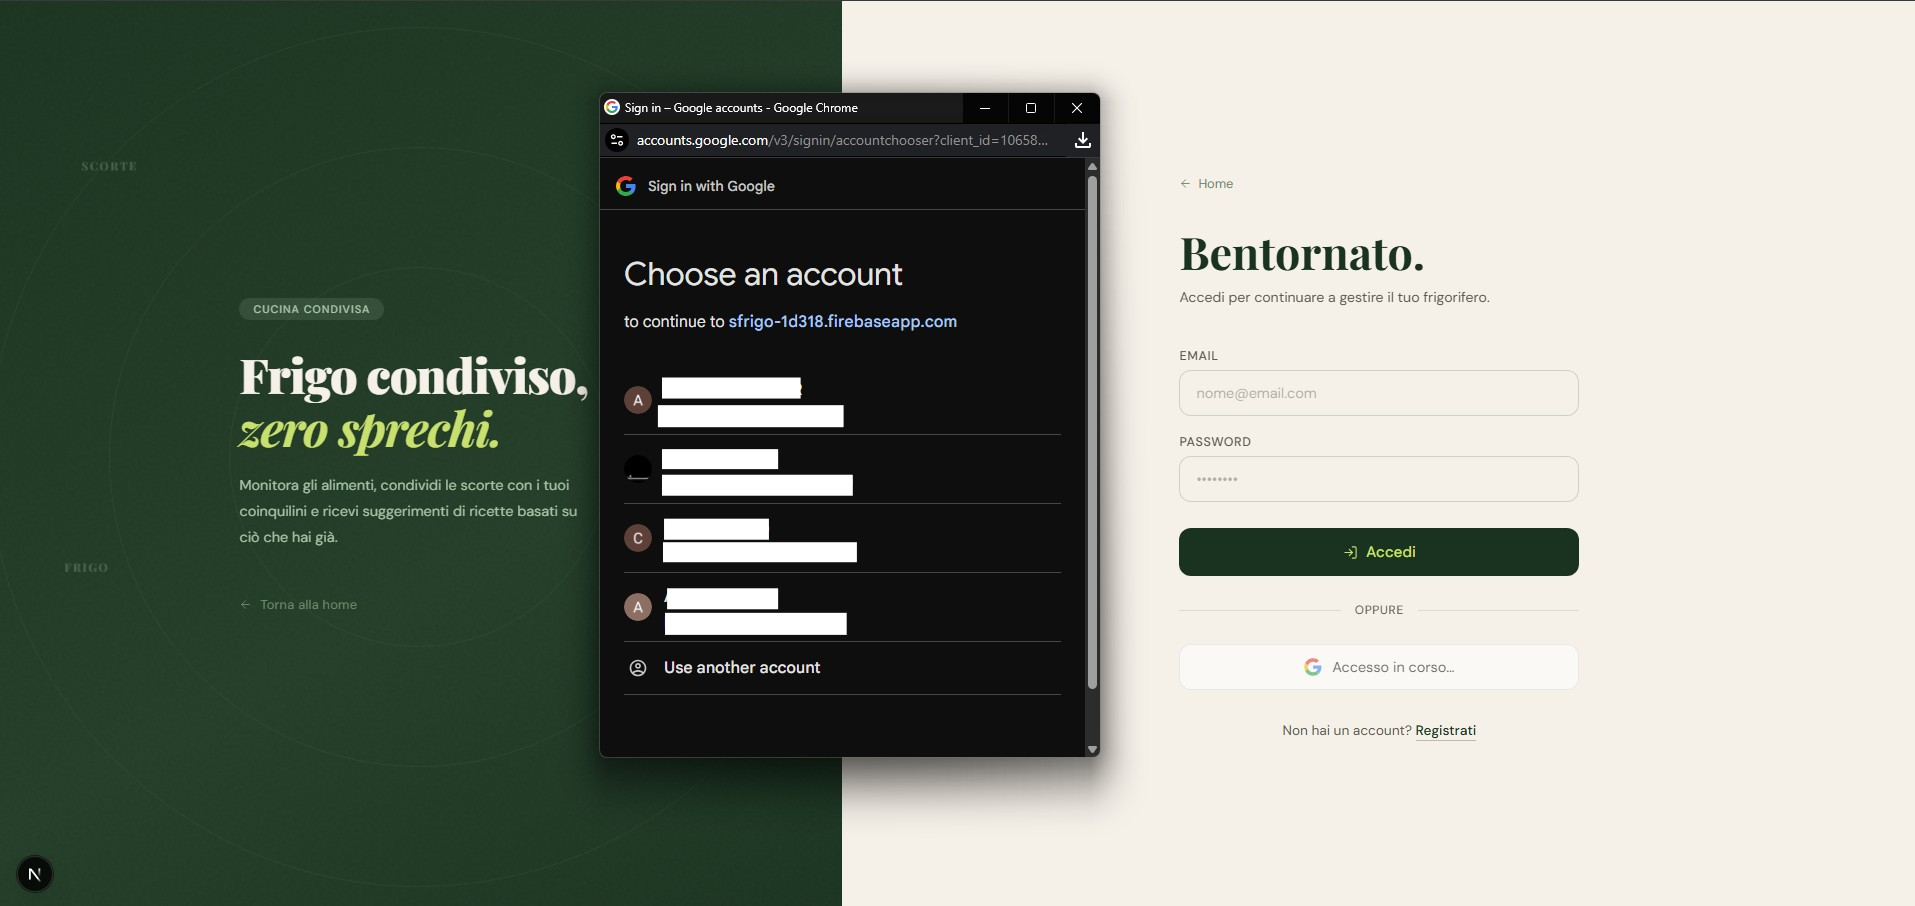
\includegraphics[width=\textwidth]{./img/login.jpg}
  \caption{Schermata di Login}
  \label{fig:login}
\end{figure}

\begin{figure}[H]
  \centering
  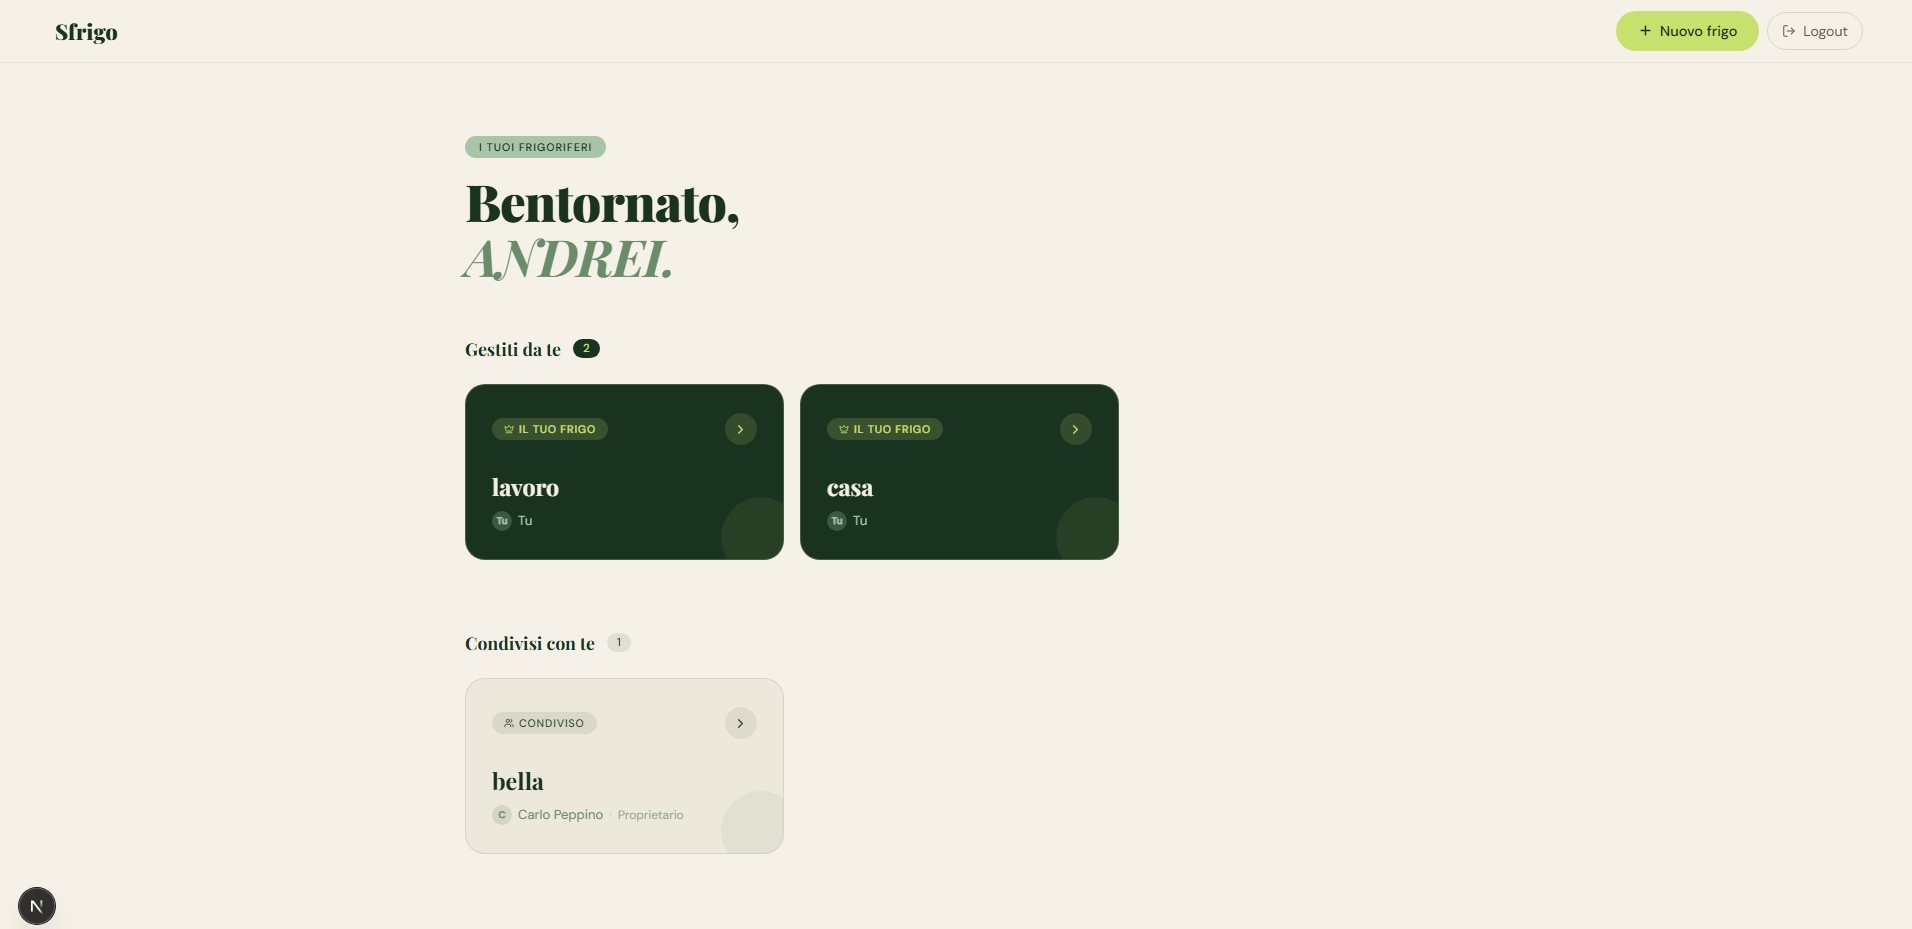
\includegraphics[width=0.93\textwidth]{./img/dashboard.jpg}
  \caption{Dashboard: i tuoi frigoriferi condivisi}
  \label{fig:dashboard}
\end{figure}

\begin{figure}[H]
  \centering
  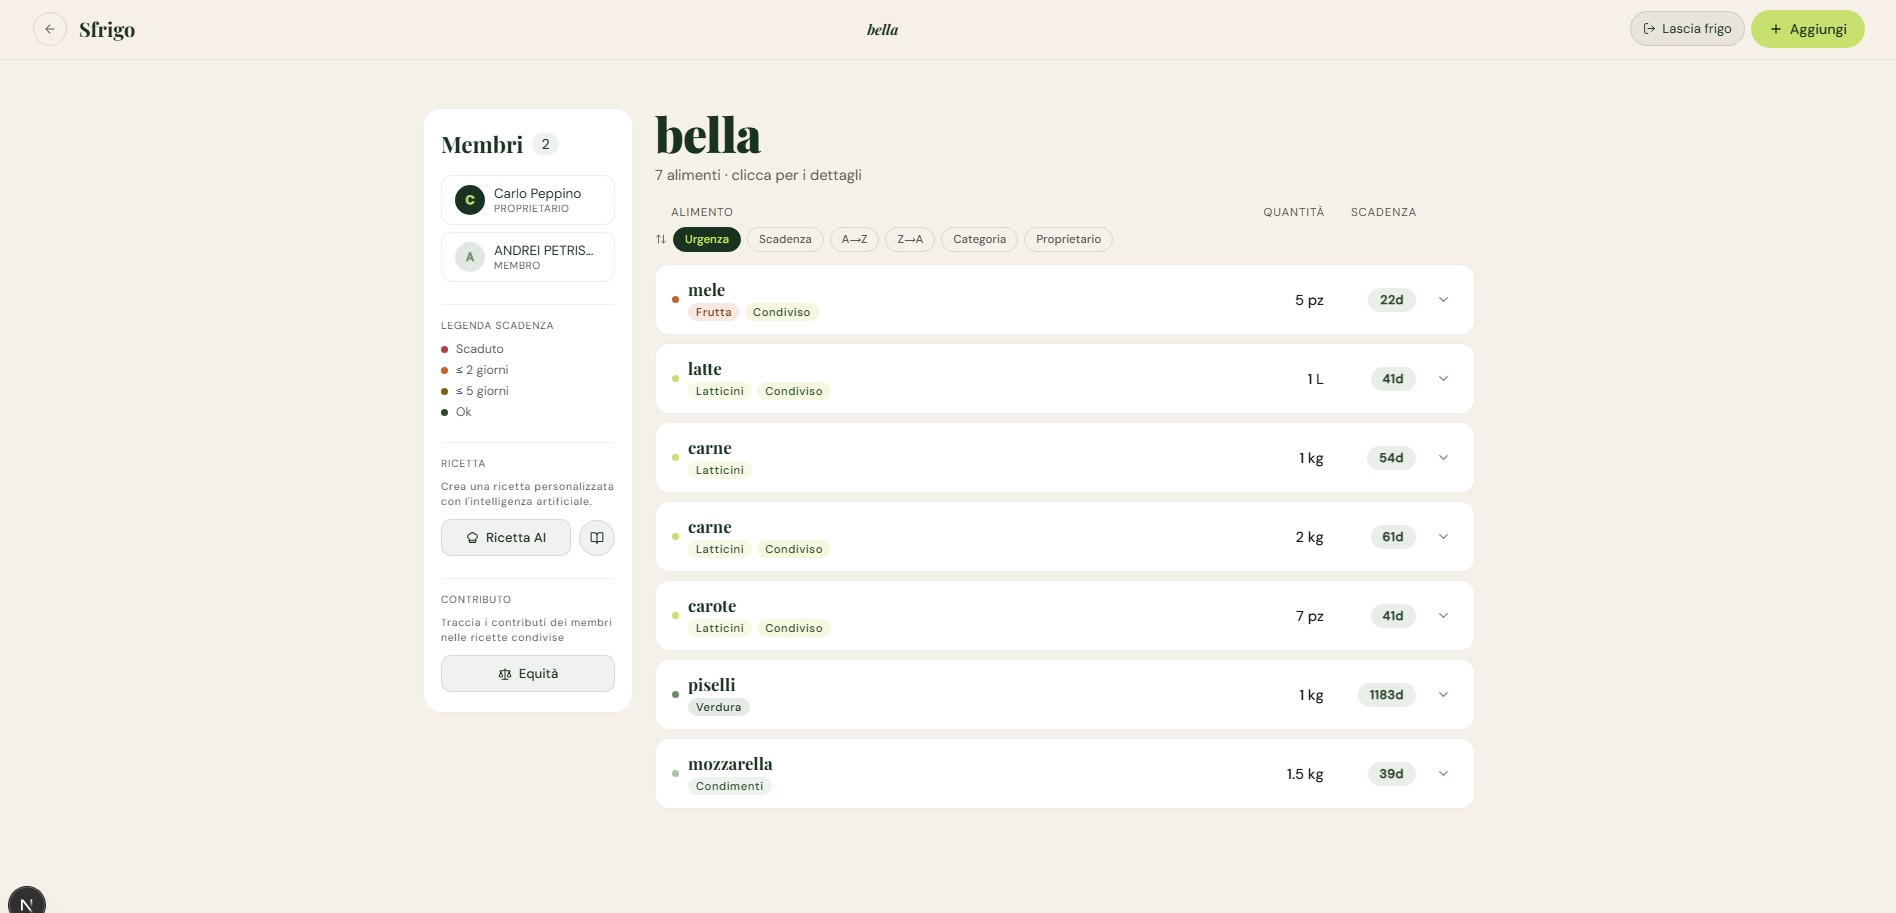
\includegraphics[width=0.93\textwidth]{./img/inventario.jpg}
  \caption{Inventario del frigorifero con modalità di ordinamento per urgenza}
  \label{fig:inventario}
\end{figure}

\begin{figure}[H]
  \centering
  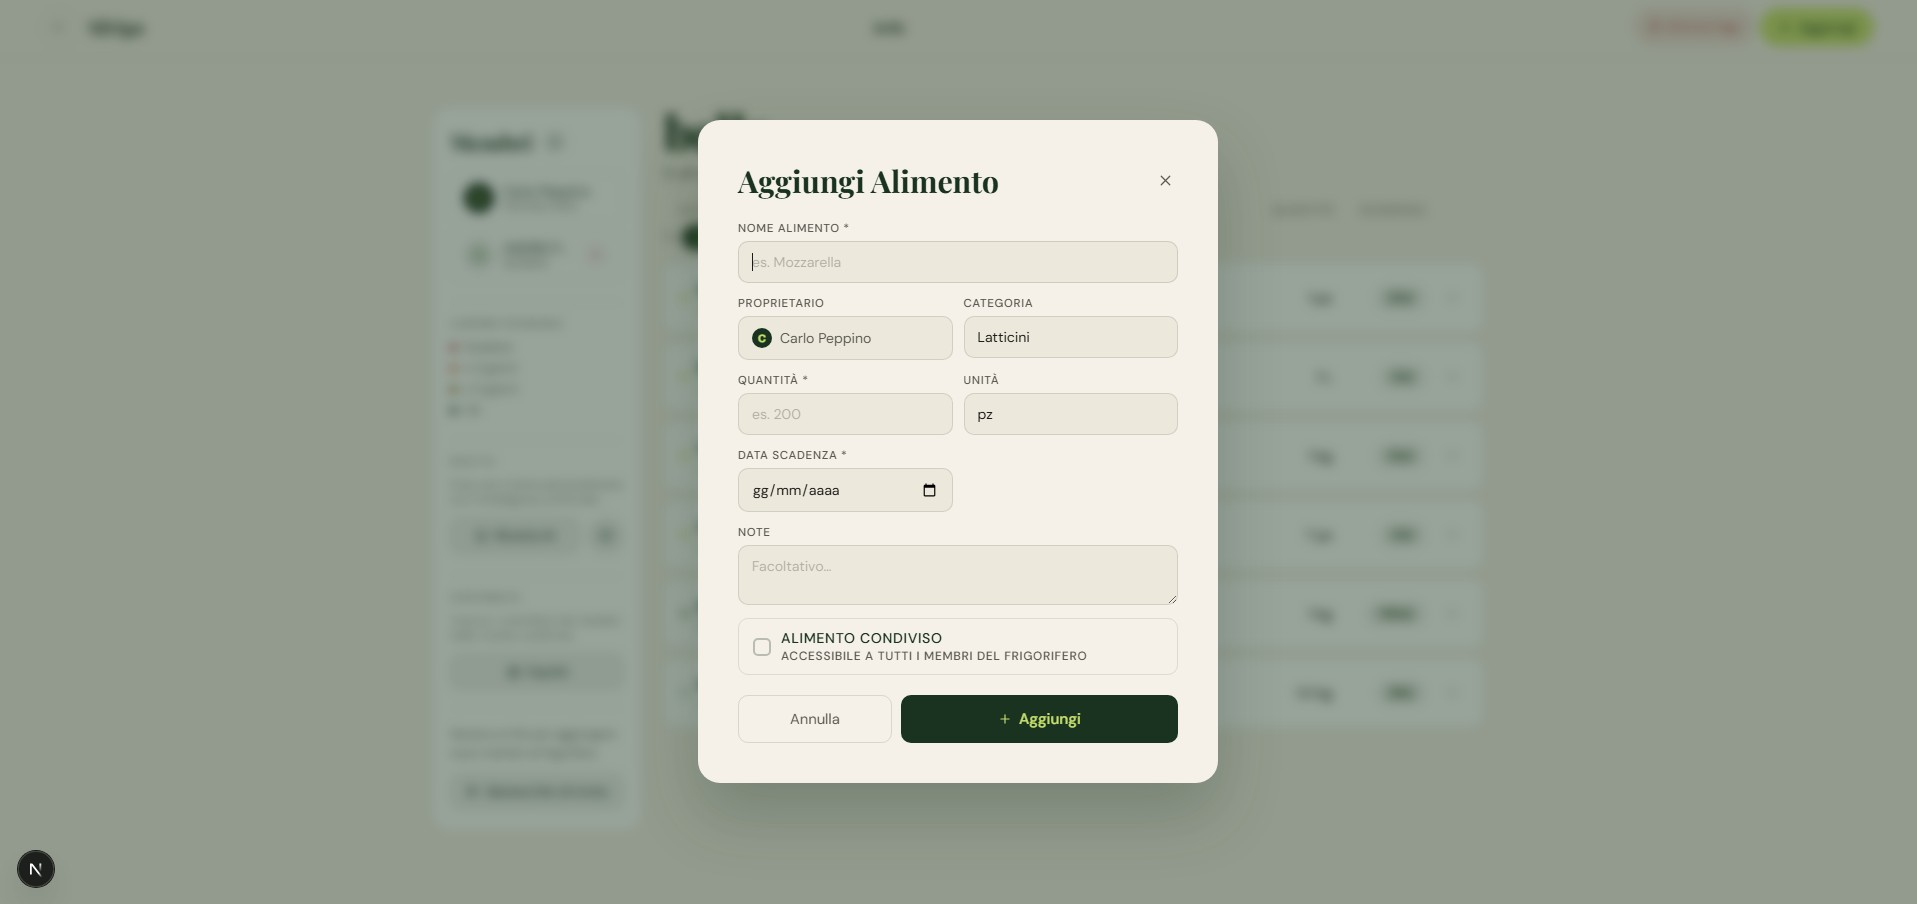
\includegraphics[width=0.93\textwidth]{./img/aggiungi alimento.jpg}
  \caption{Aggiungi Alimento}
  \label{fig:aggiungi-alimento}
\end{figure}

\begin{figure}[H]
  \centering
  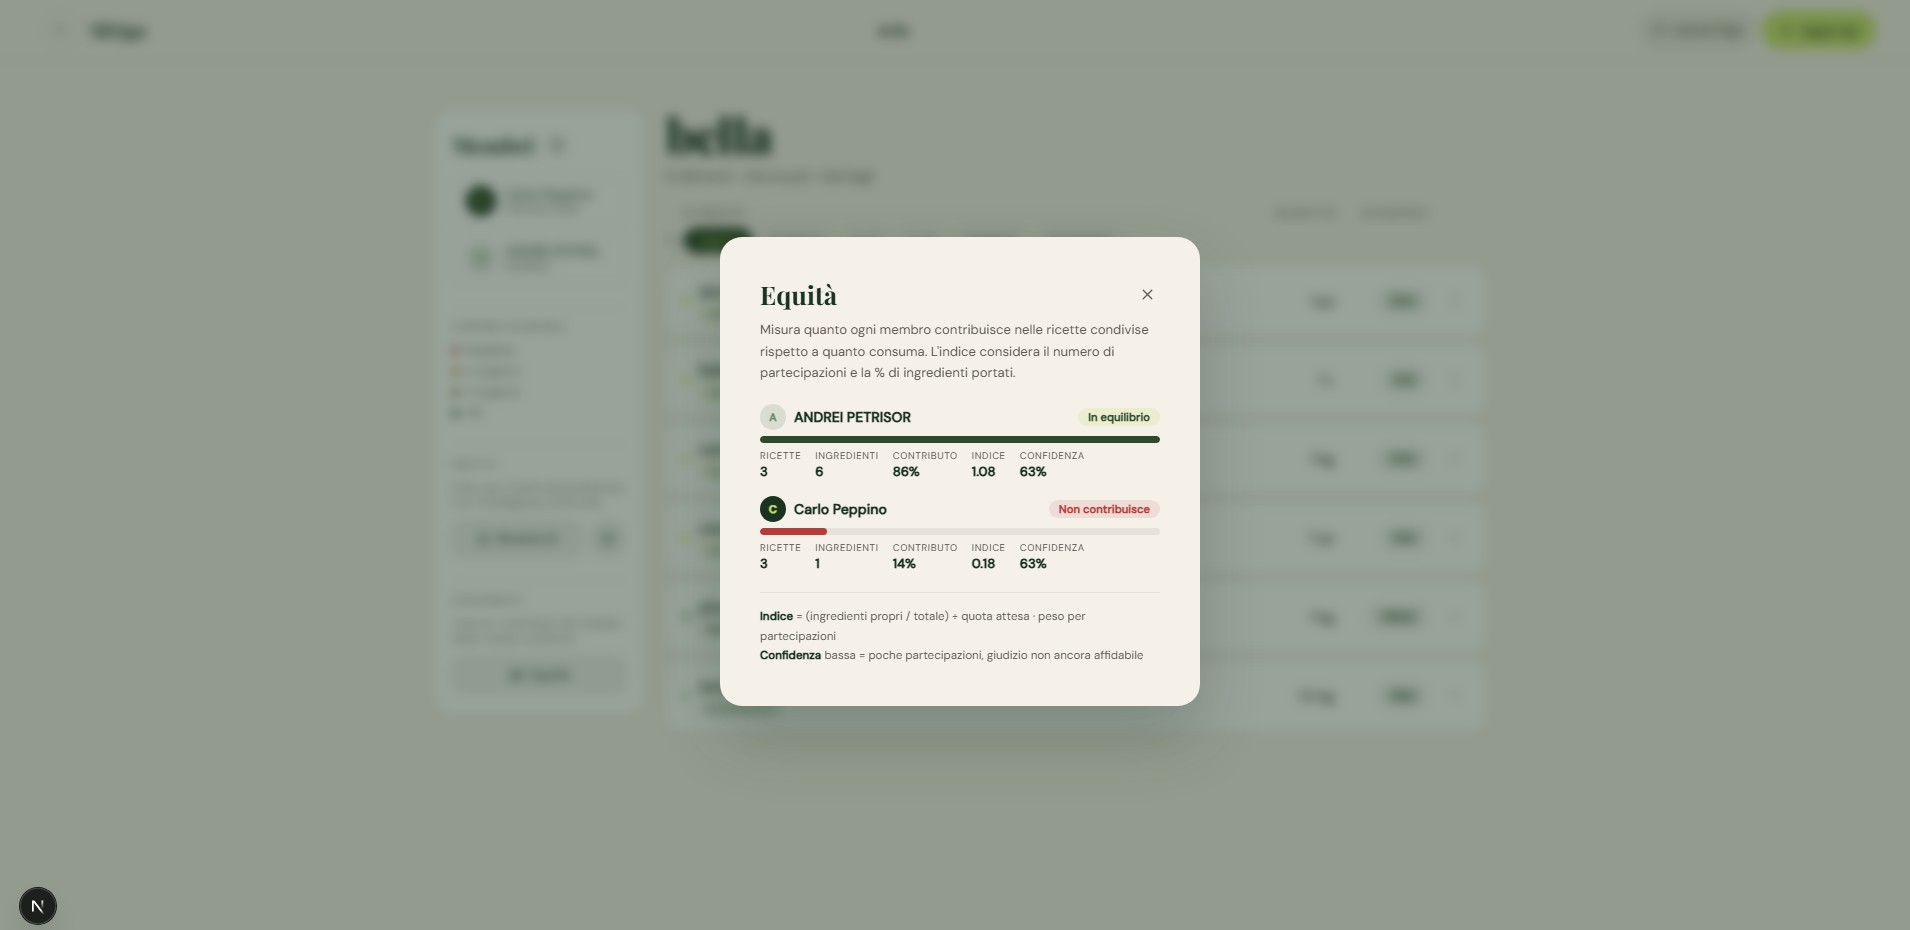
\includegraphics[width=0.93\textwidth]{./img/equità.jpg}
  \caption{Algoritmo di equity}
  \label{fig:equity}
\end{figure}

\begin{figure}[H]
  \centering
  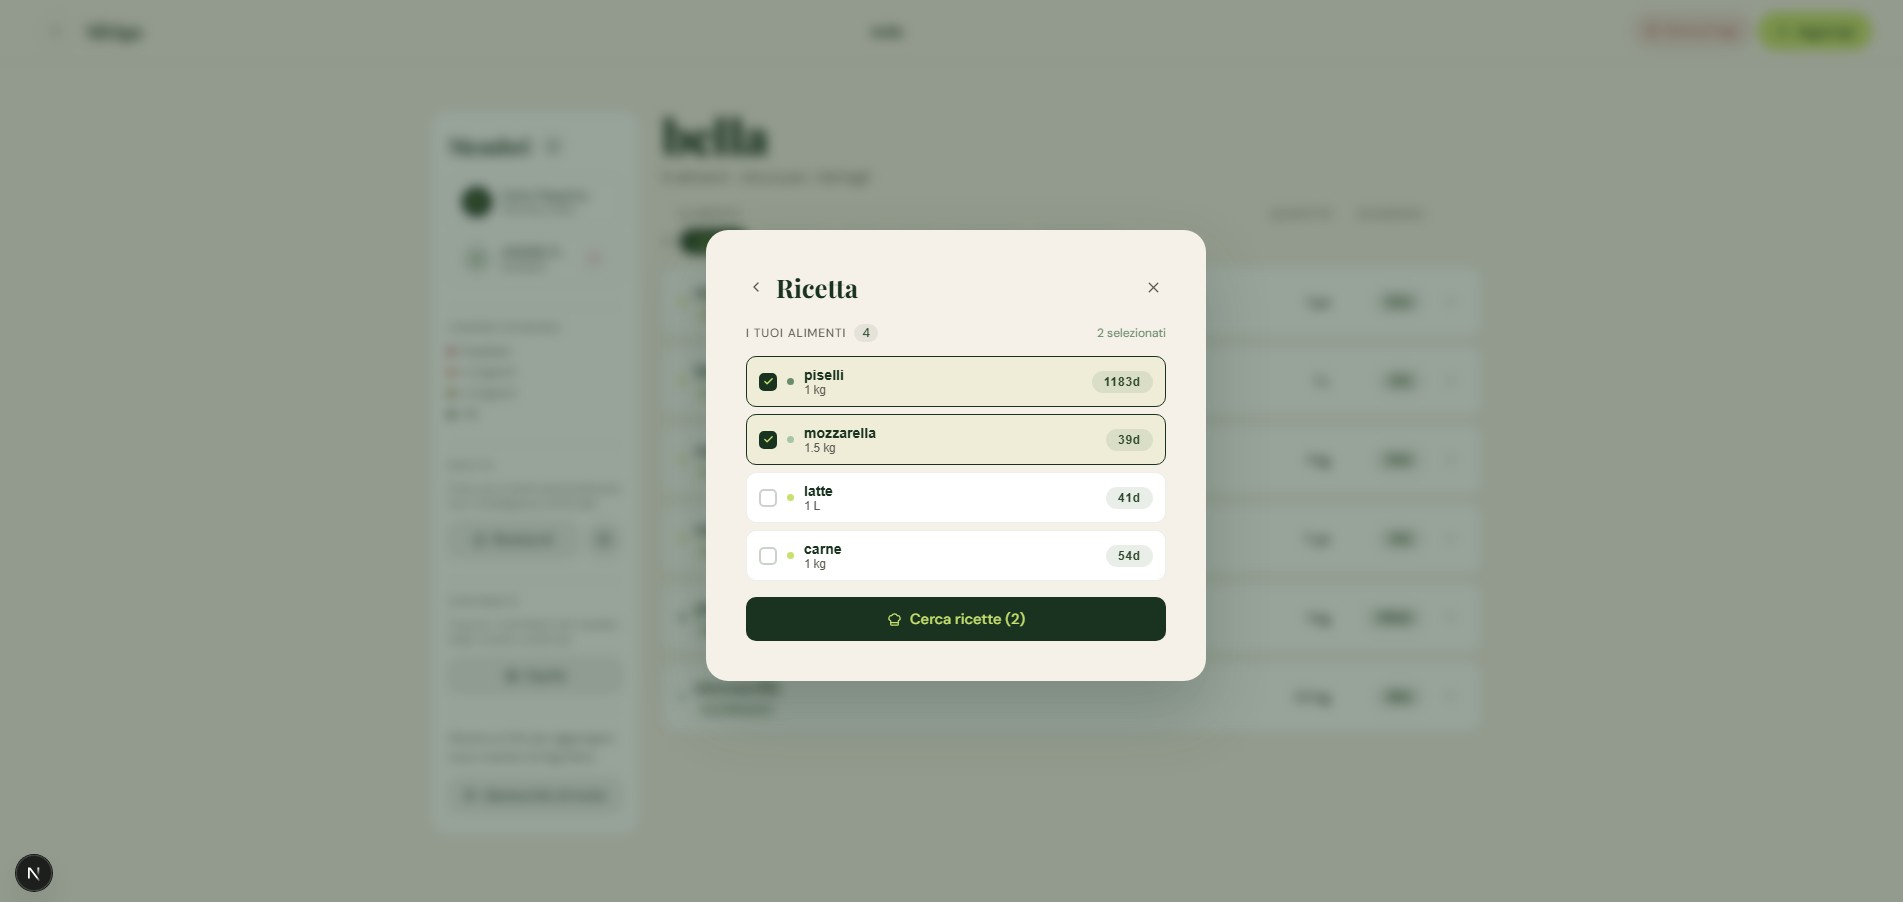
\includegraphics[width=0.93\textwidth]{./img/ricetta.jpg}
  \caption{Ricetta: visualizzazione e modifica}
  \label{fig:ricetta}
\end{figure}

\begin{figure}[H]
  \centering
  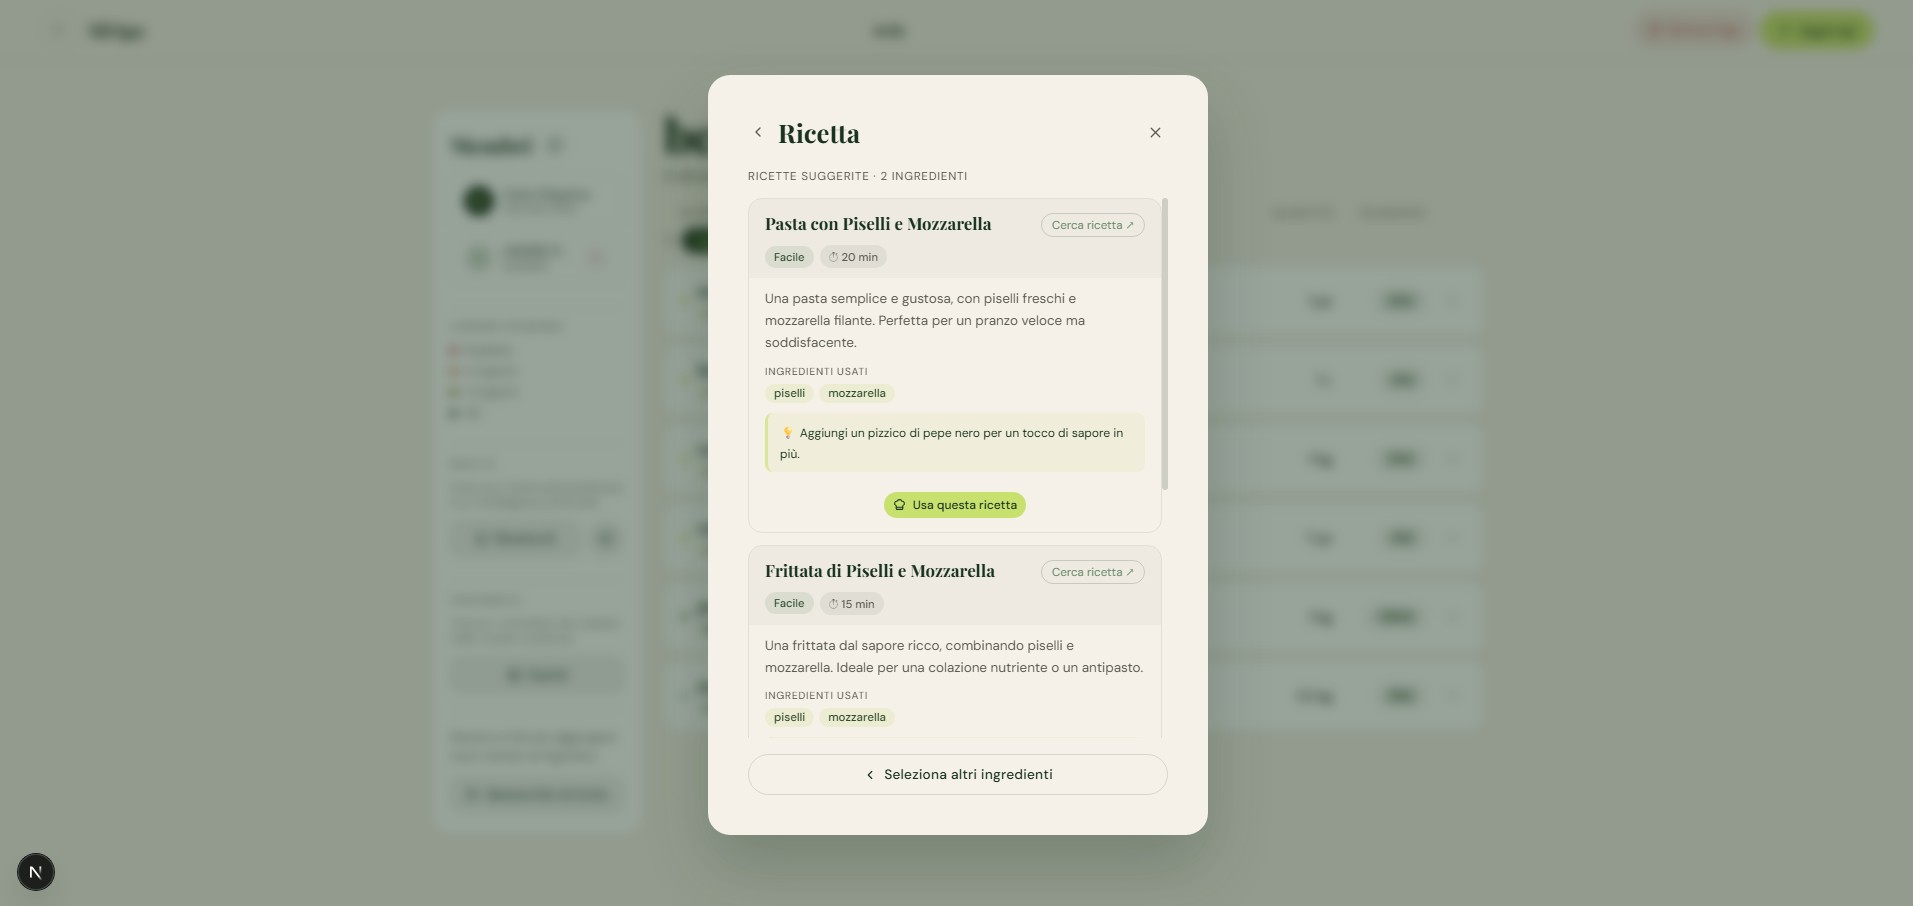
\includegraphics[width=0.93\textwidth]{./img/ricette suggerite.jpg}
  \caption{Ricette suggerite}
  \label{fig:ricette-suggerite}
\end{figure}

\end{document}
